\documentclass[a4paper,12pt]{article}
\title{\heiti 物理海洋学笔记}
\author{\small 2017级海洋科学专业 崔英哲 \quad cuiyingzhe@stu.ouc.edu.cn\\
 \small \url{https://github.com/Cuiyingzhe/OUC-Physical-Oceanography-Notes}}
\date{\small 2020.07.06}
\usepackage[UTF8]{ctex}
%\usepackage{indentfirst}
\usepackage{geometry}
\usepackage{amsmath}
\usepackage{booktabs}
\usepackage{tabu}
\usepackage{caption}
%\usepackage{gensymb}
\usepackage{graphicx}
\usepackage{float}
\usepackage{cite}
\usepackage{hyperref}
\usepackage{cases}
\usepackage{esint}
\usepackage{fancyhdr}
\usepackage{CJK}
\usepackage{titlesec}
\usepackage{titletoc}
\usepackage{mathrsfs}
\usepackage{harpoon}
\usepackage{amssymb}
\usepackage{color}
\usepackage{bm}
\usepackage{framed}
\usepackage{setspace}
\usepackage{gensymb}
\usepackage{tikz}
\usepackage{cancel}
\usepackage{multicol}
\usepackage{subfigure}
\newcommand*{\circled}[1]{\lower.7ex\hbox{\tikz\draw (0pt, 0pt)%
    circle (.5em) node {\makebox[1em][c]{\small #1}};}}
\newcommand\prt[2]{$\frac{\partial #1}{\partial #2}$}
%\usepackage[T1]{fontenc}
%\usepackage{mathptmx}
\hypersetup{
	colorlinks=true,
	linkcolor=black,
	citecolor=blue
}
\captionsetup[table]{labelsep=space,font={small}}
\captionsetup[figure]{labelsep=space,font={small}}
\captionsetup[subfigure]{labelsep=space,font={small}}
\geometry{a3paper,left=4cm,right=4cm,top=4cm,bottom=4cm}
\graphicspath{{C:/Users/Gary/Desktop/OUC-Physical-Oceanography-Notes/figures/}}
\begin{document}
    \maketitle
    \renewcommand*\contentsname{}
	\tableofcontents
    \newpage
    \section{基本方程}
    \subsection{旋转坐标系的速度和加速度}
    \setlength{\parindent}{0pt}
    惯性坐标系:
    静止的或是匀速直线运动的坐标系,固定在恒星上的坐标系可以被看成惯性坐标系.\\
    固定在地球上的坐标系:
    地球对恒星的加速度主要是由地球自转引起的,于是可以把地球当作一个对惯性坐标系作纯粹地转运动的物体.
    \subsubsection{旋转坐标系和惯性坐标系中的速度}
    \begin{figure}[H]
		\centering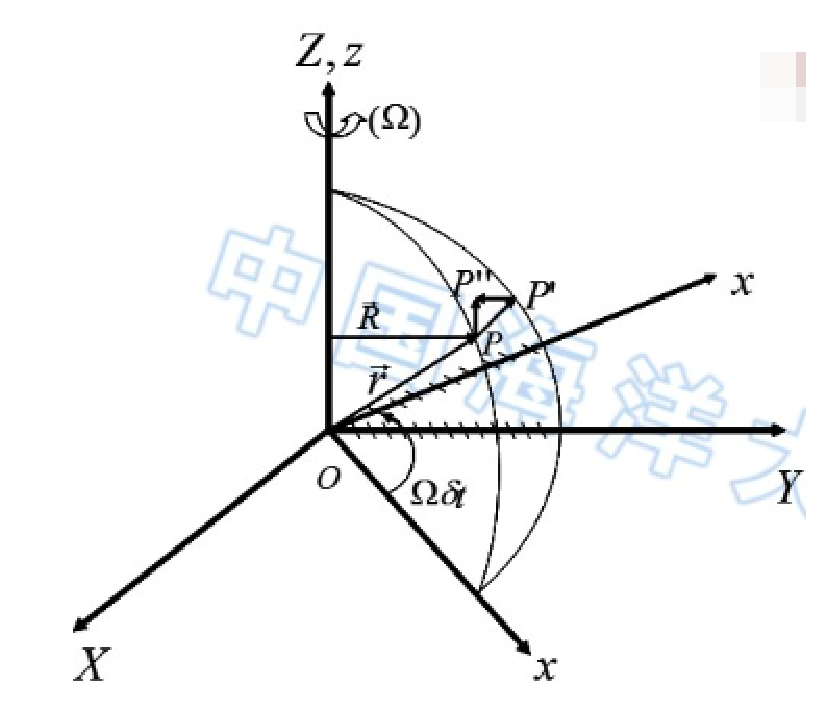
\includegraphics[width=7cm]{1.eps}
		\caption*{}
    \end{figure}
    惯性坐标系($XYZ$)绝对位移:$\vec{pp''}=\vec{V}_a\delta t, \vec{V}_a$为绝对速度\\
    旋转坐标系($xyz$)相对位移:$\vec{p'p''}=\vec{V}\delta t, \vec{V}$为相对速度\\
    $\because \vec{pp''}=\vec{p'p''}+\vec{pp'}$ \\
    $\therefore\vec{V}_a\delta t=\vec{V}\delta t+\vec{V}_e\delta t\Rightarrow\vec{V}_a=\vec{V}+\vec{V}_e$(绝对速度等于相对速度与牵连速度的向量和)\\
    其中,$\vec{V}_e=\vec{\Omega}\times\vec{r}\Rightarrow\vec{V}_a=\vec{V}+\vec{\Omega}\times\vec{r}$
    \[
        \Rightarrow\frac{d_a\vec{r}}{dt}=\frac{d\vec{r}}{dt}+\vec{\Omega}\times\vec{r}
    \]
    \[
        \frac{d_a\vec{A}}{dt}=\frac{d\vec{A}}{dt}+\vec{\Omega}\times\vec{A}
    \]
    \subsubsection{旋转坐标系和惯性坐标系中的加速度}
    令$\vec{A}=\vec{V}_a=\vec{V}_e+\vec{V}=\vec{V}+\vec{\Omega}\times\vec{r}$
    \begin{equation*}
        \begin{aligned} \frac{d \bar{V}_{a}}{d t} &=\frac{d_{a}}{d t}\left(\vec{V}+\vec{V}_{e}\right)=\frac{d_{a}}{d t}(\vec{V}+\vec{\Omega} \times \vec{r}) \\ &=\frac{d}{d t}(\vec{V}+\vec{\Omega} \times \vec{r})+\vec{\Omega} \times(\vec{V}+\vec{\Omega} \times \vec{r}) \\ &=\frac{d \vec{V}}{d t}+\vec{\Omega} \times \vec{V}+\vec{\Omega} \times \vec{V}+\vec{\Omega} \times(\vec{\Omega} \times \vec{r}) \\ &=\frac{d \vec{V}}{d t}+2 \vec{\Omega} \times \vec{V}-\Omega^{2} \vec{R} \end{aligned}
    \end{equation*}
    \subsection{作用在海水微团上的外力 运动方程的向量形式}
    压强梯度力:$\displaystyle\frac{1}{\rho}\nabla p$\\
    分子粘性力(摩擦力):
    \[
        \left\{
        \begin{aligned}
            &F_{x}=\frac{1}{\rho} \mu\left(\frac{\partial^{2} u}{\partial x^{2}}+\frac{\partial^{2} u}{\partial y^{2}}+\frac{\partial^{2} u}{\partial z^{2}}\right)=\frac{\mu}{\rho} \Delta u\\
            &F_{y}=\frac{1}{\rho} \mu\left(\frac{\partial^{2} v}{\partial x^{2}}+\frac{\partial^{2} v}{\partial y^{2}}+\frac{\partial^{2} v}{\partial z^{2}}\right)=\frac{\mu}{\rho} \Delta v\\
            &F_{2}=\frac{1}{\rho} \mu\left(\frac{\partial^{2} w}{\partial x^{2}}+\frac{\partial^{2} w}{\partial y^{2}}+\frac{\partial^{2} w}{\partial z^{2}}\right)=\frac{\mu}{\rho} \Delta w
        \end{aligned}
        \right.
        \Rightarrow \vec{F}=\frac{\mu}{\rho}\Delta \vec{V}=\nu\Delta\vec{v}
    \]
    重力(地球引力与地球自转产生的惯性离心力的合力):$\displaystyle\vec{g}=-G\frac{M_g}{r^2}\cdot\left(\frac{\vec{r}}{r}\right)$\\
    科氏力:$\displaystyle -2\vec{\Omega}\times\vec{V}$\\
    天体引潮力(受其他天体万有引力与惯性力离心力的合力):$\displaystyle\vec{F_M}=-G\frac{M}{L^2}+G\frac{M}{D^2}\cdot\left(\frac{\vec{D}}{D}\right)$\\
    由牛顿第二定律和坐标系转换关系:
    \[
        \left\{
        \begin{aligned}
            &\frac{d_{a} \vec{V}_{a}}{d t}=\sum_{i} \vec{F}_{t}\\
            &\frac{d_{a} \vec{A}_{a}}{d t}=\frac{d \vec{V}}{d t}+2 \vec{\Omega} \times \vec{V}-\Omega^{2} \vec{R}
        \end{aligned}
        \right.
    \]
    \[
        \Rightarrow\boxed{\color{red} \frac{d \vec{V}}{d t}=-\frac{1}{\rho} \nabla P-2 \vec{\Omega} \times \vec{V}+\vec{g} +\nu \Delta \vec{V}+\vec{F}_{M}}
    \]
    \subsection{运动方程在球坐标系的标量形式}
    \begin{figure}[H]
        \centering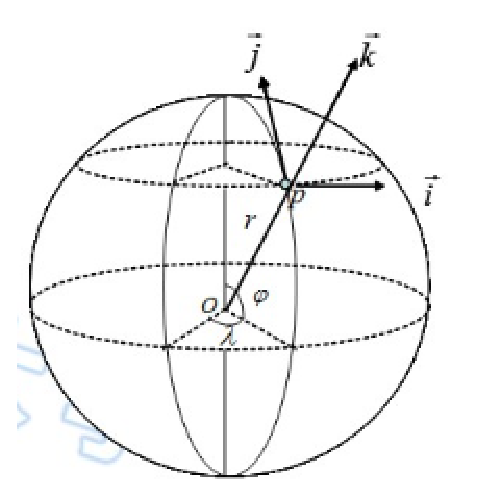
\includegraphics[width=5cm]{2.eps}
        \caption*{}
    \end{figure}
    速度:
    \[
        \vec{V}=u\vec{i}+v\vec{j}+w\vec{k}
    \]
    \[
        \Rightarrow
        \left\{\begin{array}{l}u=r \cos \varphi \frac{d \lambda}{d t} \\ v=r \frac{d \varphi}{d t} \\ w=\frac{d r}{d t}\end{array}\right.
    \]
    加速度:
    \[
        \begin{aligned}
        \frac{d\vec{A}}{dt}&=\frac{\frac{\partial \vec{A}}{\partial t} d t+\frac{\partial \vec{A}}{\partial \lambda} d \lambda+\frac{\partial \vec{A}}{\partial \varphi} d \varphi+\frac{\partial \vec{A}}{\partial r} d r}{dt}\\
        &=\frac{\partial \bar{A}}{\partial t}+\frac{\partial \vec{A}}{\partial \lambda} \frac{d \lambda}{d t}+\frac{\partial \vec{A}}{\partial \varphi} \frac{d \varphi}{d t}+\frac{\partial \vec{A}}{\partial r} \frac{d r}{d t}\\
        &=\frac{\partial \vec{A}}{\partial t}+\frac{u}{r \cos \varphi} \frac{\partial \vec{A}}{\partial \lambda}+\frac{v}{r} \frac{\partial \vec{A}}{\partial \varphi}+w \frac{\partial \vec{A}}{\partial r}
        \end{aligned}
    \]
    \[
        \begin{aligned}
        &\Rightarrow\frac{d}{d t}=\frac{\partial}{\partial t}+u \frac{\partial}{r \cos \varphi \partial \lambda}+v \frac{\partial}{r \partial \varphi}+w \frac{\partial}{\partial r}\\
        &\Rightarrow\boxed{\bm{ \frac{d}{d t}=\frac{\partial}{\partial t}+(\vec{V} \cdot \nabla)}}\\
        &\Rightarrow\boxed{\bm{ \nabla=\frac{\partial}{r \cos \varphi \partial \lambda} \vec{i}+\frac{\partial}{r \partial \varphi} \vec{j}+\frac{\partial}{\partial r} \vec{k}}}
        \end{aligned}
    \]
    \[
        \Rightarrow
        \left\{
            \begin{aligned}
                &\frac{d \vec{i}}{d t}=\frac{\partial \vec{i}}{\partial t}+u \frac{\partial \vec{i}}{r \cos \varphi \partial \lambda}+v \frac{\partial \vec{i}}{r \partial \varphi}+w \frac{\partial \vec{i}}{\partial r}\\
                &\frac{\partial \vec{j}}{d t}=\frac{\partial \vec{j}}{\partial t}+u \frac{\partial \vec{j}}{r \cos \varphi \partial \lambda}+v \frac{\partial \vec{j}}{r \partial \varphi}+w \frac{\partial \vec{j}}{\partial r}\\
                &\frac{d \vec{k}}{d t}=\frac{\partial \vec{k}}{\partial t}+u \frac{\partial \vec{k}}{r \cos \varphi \partial \lambda}+v \frac{\partial \vec{k}}{r \partial \varphi}+w \frac{\partial \vec{k}}{\partial r}
            \end{aligned}
        \right.
    \]
    \newpage
    \[
        \begin{aligned}
            &\frac{d \vec{V}}{d t}=\frac{d u}{d t} \vec{i}+\frac{d v}{d t} \vec{j}+\frac{d v}{d t} \vec{k}+u \frac{d \vec{i}}{d t}+v \frac{d \vec{j}}{d t}+w \frac{d \vec{k}}{d t}\\
            \Rightarrow&\boxed{\color{red}\frac{d \vec{V}}{d t}=\left(\frac{d u}{d t}-\frac{u v t g \varphi}{r}+\frac{u w}{r}\right) \vec{i}+\left(\frac{d v}{d t}+\frac{u^{2} \operatorname{tg} \varphi}{r}+\frac{v w}{r}\right) \vec{j}+\left(\frac{d w}{d t}-\frac{u^{2}+v^{2}}{r}\right)}
        \end{aligned}
    \]
    压强梯度力:
    \[
        \frac{1}{\rho}\nabla p=-\frac{1}{\rho}\left(\frac{1}{r \cos \varphi} \frac{\partial p}{\partial \lambda} \vec{i}+\frac{1}{r} \frac{\partial p}{\partial \varphi} \vec{j}+\frac{\partial p}{\partial r} \vec{k}\right)
    \]
    重力:
    \[
        \vec{g}=-g\vec{k}
    \]
    科氏力:
    \begin{figure}[H]
        \centering 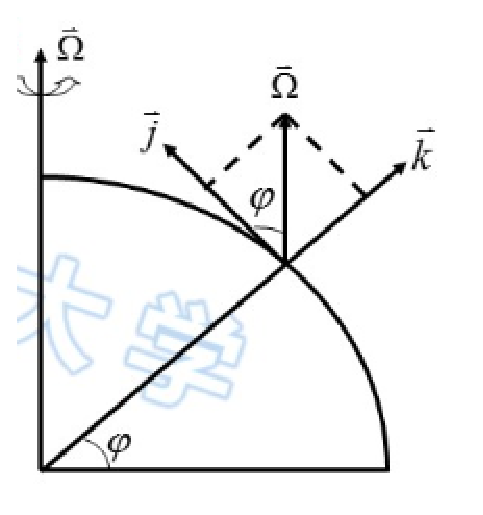
\includegraphics[width=4cm]{3.eps}
        \caption*{}
    \end{figure}
    \vspace{-2cm}
    \[
        \vec{\Omega}=\Omega \sin \varphi \vec{k}+\Omega \cos \varphi \vec{j}
    \]
    \[
        \begin{aligned}
            -2 \vec{\Omega} \times \vec{V}&=-2\left|\begin{array}{ccc}\vec{i} & \vec{j} & \vec{k} \\ 0 & \Omega \cos \varphi & \Omega \sin \varphi \\ u & v & w\end{array}\right|\\
            &=-2[(w \Omega \cos \varphi-v \Omega \sin \varphi) \vec{i}+(u \Omega \sin \varphi) \vec{j}+(-u \Omega \cos \varphi) \vec{k}]
        \end{aligned}
    \]
    \[
        \Rightarrow-2 \vec{\Omega} \times \vec{V}=(f v-\tilde{f} w) \vec{i}-(f u) \vec{j}+(\tilde{f} u) \vec{k}
    \]
    其中,$\displaystyle\left\{\begin{aligned}&f=2\Omega \sin\varphi\\ &\tilde{f}=2\Omega \cos\varphi\end{aligned}\right.$
    \[
        \Rightarrow
        \boxed{
        \left\{
        \begin{aligned}
            &\frac{d u}{d t}=-\frac{1}{\rho} \frac{\partial p}{r \cos \varphi \partial \lambda}+f v-\tilde{f} w+\frac{u v \tan \varphi}{r}-\frac{u w}{r}+\gamma(\Delta \vec{v})_{\lambda}-\frac{1}{r \cos \varphi} \frac{\partial \phi_{T}}{\partial \lambda}\\
            &\frac{d y}{d t}=7 \frac{1}{\rho} \frac{\partial p}{r \partial \varphi}-f u-\frac{u^{2} \tan \varphi}{r}-\frac{v w}{r}+\gamma(\Delta \bar{v})_{\varphi}-\frac{1}{r} \frac{\partial \phi_{T}}{\partial \varphi}\\
            &\frac{d w}{d t}=-\frac{1}{\rho} \frac{\partial p}{\partial r}+\tilde{f} u=g+\frac{u^{2}+v^{2}}{r}+\gamma(\Delta \vec{v})_{r}-\frac{\partial \phi_{T}}{\partial r}
        \end{aligned}
        \right.
        }
    \]
    \subsection{直角坐标系的运动方程}
    略去地球曲率的影响
    \[
        \Rightarrow
        \boxed{
        \left\{
        \begin{aligned}
            &\frac{d u}{d t}=-\frac{1}{\rho} \frac{\partial p}{\partial x}+f v+\tilde{f} w+F_{N \lambda}+F_{T \lambda}\\
            &\frac{d v}{d t}=-\frac{1}{\rho} \frac{\partial p}{\partial x}-f u+F_{N y}+F_{T y}\\
            &\frac{d w}{d t}=-\frac{1}{\rho} \frac{\partial p}{\partial z}+\tilde{f} u-g+F_{N z}+F_{T z}
        \end{aligned}
        \right.
        }
    \]
    \subsection{海水层流运动的基本方程组}
    \subsubsection{连续方程}
    \[
        \frac{\partial \rho}{\partial t}+\nabla \cdot(\rho \vec{V})=0 \Leftrightarrow \frac{d \rho}{d t}+\rho \nabla \cdot \vec{V}=0
    \]
    特别地,对于不可压缩流体:
    \[
        \nabla \cdot \vec{V}=0
    \]
    \subsubsection{盐量扩散方程}
    \[
        \mathop{\frac{\partial}{\partial t} \iiint\limits_{\tau} \rho s d \tau}\limits^{\mbox{盐量增加量}}=\mathop{-\oiint\limits_{\sigma} \rho s V_{n} d \sigma}\limits^{\mbox{平流作用}}+\mathop{-\oiint\limits_{\sigma} S_{n} d \sigma}\limits^{\mbox{分子扩散作用}}
    \]
    \[
        \begin{aligned}
            &\iiint\limits_{\tau} \frac{\partial (\rho s)}{\partial t} d \tau =\iiint\limits_{\tau} \nabla \cdot(\rho s \vec{V}) d \tau -\iiint\limits_{\tau} \nabla \cdot \vec{S} d \tau \\
            \Rightarrow&\frac{\partial(\rho s)}{\partial t}+\nabla \cdot(\rho s \vec{V})+\nabla \cdot \vec{S}=0\\
            \Rightarrow&\rho \frac{\partial s}{\partial t}+s \frac{\partial \rho}{\partial t}+s \nabla \cdot(\rho \vec{V})+\rho \vec{V} \cdot \nabla s+\nabla \cdot \vec{S}=0\\
            \Rightarrow&\left(\frac{\partial s}{\partial t}+\vec{V} \cdot \nabla s\right)+\frac{s}{\rho}\left[\frac{\partial \rho}{\partial t}+\nabla \cdot(\rho \vec{V})\right]=-\frac{1}{\rho} \nabla \cdot \vec{S}\\
            \Rightarrow&\frac{\partial s}{\partial t}+\vec{V} \cdot \nabla s=\frac{k}{\rho} \Delta s=k_{D} \Delta s
        \end{aligned}
    \]
    其中,$\displaystyle k_{D}=\frac{k}{\rho} \sim 1.1 \times 10^{-9}\left(\mathrm{m}^{2} / \mathrm{s}\right)$
    \subsubsection{热传导方程}
    与上面类似:
    \[
        \frac{\partial \theta}{\partial t}+\vec{V} \cdot \nabla \theta=\frac{\kappa}{\rho c_{p}} \Delta \theta=k_{\theta} \Delta \theta
    \]
    其中,$\displaystyle k_{\theta}=\frac{\kappa}{\rho c_{p}} \sim 1.4 \times 10^{-7}\left(\mathrm{m}^{2} / \mathrm{s}\right)$
    \subsubsection{热膨胀方程-状态方程}
    热膨胀方程:
    \[
        \rho=\mathop{\rho_0}\limits^{\mbox{0℃时的海水密度}}(1-\mathop{k} \limits^{\mbox{海水的热膨胀系数}} \theta)
    \]
    EOS80国际海水状态方程:
    \[
        \rho(s, t, p)=\rho(s, t, 0)\left[1-\frac{n p}{k(s, t, p)}\right]^{-1}
    \]
    \subsection{基本方程的矢量形式和标量形式}
    矢量形式:
    \[
        \boxed{
        \color{red}
        \left\{
        \begin{aligned}
            &\frac{d \vec{V}}{d t}=-\frac{1}{\rho} \nabla p-2 \Omega \times \vec{V}+\vec{g}+\gamma \Delta \vec{V}-\nabla \phi_{T}\\
            &\frac{\partial \rho}{\partial t}+\rho \nabla \cdot \vec{V}=0\\
            &\frac{\partial s}{\partial t}+\vec{V} \cdot \nabla s=k_{D} \Delta s\\
            &\frac{\partial \theta}{\partial t}+\vec{V} \cdot \nabla \theta={k}_{\theta} \Delta \theta\\
            &\rho=\rho(\theta, s, p)
        \end{aligned}
        \right.
        }
    \]
    标量形式(直角坐标系):
    \[
        \boxed{
        \color{red}
        \left\{
        \begin{aligned}
            &\frac{d v}{d t}=-\frac{1}{\rho} \frac{\partial p}{\partial y}-f u+\gamma \Delta v-\frac{\partial \phi_{T}}{\partial y}\\
            &\frac{d w}{d t}=-\frac{1}{\rho} \frac{\partial p}{\partial z}+\tilde{f} u-g+\gamma \Delta w-\frac{\partial \phi_{T}}{\partial z}\\
            &\frac{d \rho}{d t}+\rho\left(\frac{\partial {u}}{\partial {x}}+\frac{\partial {v}}{\partial {y}}+\frac{\partial {w}}{\partial {z}}\right)=0\\
            &\frac{\partial s}{\partial t}+u \frac{\partial s}{\partial x}+v \frac{\partial s}{\partial y}+w \frac{\partial s}{\partial z}=k_{D}\left(\frac{\partial^{2} s}{\partial x^{2}}+\frac{\partial^{2} s}{\partial y^{2}}+\frac{\partial^{2} s}{\partial z^{2}}\right)\\
            &\frac{\partial \theta}{\partial t}+u \frac{\partial \theta}{\partial x}+v \frac{\partial \theta}{\partial y}+w \frac{\partial \theta}{\partial z}=k_{\theta}\left(\frac{\partial^{2} \theta}{\partial x^{2}}+\frac{\partial^{2} \theta}{\partial y^{2}}+\frac{\partial^{2} \theta}{\partial z^{2}}\right)\\
            &\rho=\rho(\theta, s, p)
        \end{aligned}
        \right.
        }
    \]
    \subsection{边界条件}
    无质量交换的运动学边界条件:
    \[
        \frac{\partial F}{\partial t} + \vec{c} \cdot \nabla F=0
    \]
    例:\\
    (1) 海面($z=\displaystyle \zeta (x,y,t)$):$\displaystyle \frac{\partial \zeta}{\partial t}+\vec{V}_{H} \cdot \nabla_{H} \zeta-w=0$\\
    (2) 海底($\displaystyle z=-h(x,y)$): $\displaystyle \vec{V}_{H} \cdot \nabla_{H} h+w=0$\\
    动力学边界条件:\\
    由牛顿第三定律,在界面法线方向有:
    \[
        \left(\vec{p}_{n}\right)_{1}=\left(\vec{p}_{n}\right)_{2}
    \]
    \subsection{ \texorpdfstring{\color{red} $\divideontimes$} 时时间平均的基本方程和边界条件(直角坐标系)}
    \begin{framed}
    连续方程:
    \[
        \frac{\partial \bar{u}}{\partial x}+\frac{\partial \bar{v}}{\partial y}+\frac{\partial \bar{w}}{\partial z}=0
    \]
    运动方程:
    \[
        \left\{
        \begin{aligned}
            &\frac{\partial \bar{u}}{\partial t}+\bar{u} \frac{\partial \bar{u}}{\partial x}+\bar{v} \frac{\partial \bar{u}}{\partial y}+\bar{w} \frac{\partial \bar{u}}{\partial z}=-\frac{1}{\rho} \frac{\partial \bar{p}}{\partial x}+f \bar{v}-\tilde{f} \bar{w}+\gamma \Delta \bar{u}-\frac{\partial \bar{\phi}_{T}}{\partial x}+\frac{\partial}{\partial x}\left(A_{x x} \frac{\partial \bar{u}}{\partial x}\right)+\frac{\partial}{\partial y}\left(A_{x y} \frac{\partial \bar{u}}{\partial y}\right)+\frac{\partial}{\partial z}\left(A_{x z} \frac{\partial \bar{u}}{\partial z}\right)\\
            &\frac{\partial \bar{v}}{\partial t}+\vec{u} \frac{\partial \bar{v}}{\partial x}+\vec{v} \frac{\partial \bar{v}}{\partial y}+\vec{w} \frac{\partial \bar{v}}{\partial z}=-\frac{1}{\rho} \frac{\partial \bar{p}}{\partial y}-f \bar{u}+\gamma \Delta \bar{v}-\frac{\partial \bar{\phi}_{T}}{\partial y}+\frac{\partial}{\partial x}\left(A_{y x} \frac{\partial \bar{v}}{\partial x}\right)+\frac{\partial}{\partial y}\left(A_{y y} \frac{\partial \bar{v}}{\partial y}\right)+\frac{\partial}{\partial z}\left(A_{y z} \frac{\partial \bar{v}}{\partial z}\right)\\
            &\frac{\partial \bar{w}}{\partial t}+\bar{u} \frac{\partial \bar{w}}{\partial x}+\bar{v} \frac{\partial \bar{w}}{\partial y}+\bar{w} \frac{\partial \bar{w}}{\partial z}=-\frac{1}{\rho} \frac{\partial \bar{p}}{\partial z}+\tilde{f} \bar{u}-g+\gamma \Delta \bar{w}-\frac{\partial \bar{\phi}_{T}}{\partial z}+\frac{\partial}{\partial x}\left(A_{z x} \frac{\partial \bar{w}}{\partial x}\right)+\frac{\partial}{\partial y}\left(A_{z y} \frac{\partial \bar{w}}{\partial y}\right)+\frac{\partial}{\partial z}\left(A_{z z} \frac{\partial \bar{w}}{\partial z}\right)
        \end{aligned}
        \right.
    \]
    盐量扩散方程:
    \[
        \frac{\partial \bar{s}}{\partial t}+\bar{u} \frac{\partial \bar{s}}{\partial x}+\bar{v} \frac{\partial \bar{s}}{\partial y}+\bar{w} \frac{\partial \bar{s}}{\partial z}=k_{D} \Delta \bar{s}+\frac{\partial}{\partial x}\left(K_{s x} \frac{\partial \bar{s}}{\partial x}\right)+\frac{\partial}{\partial y}\left(K_{s y} \frac{\partial \bar{s}}{\partial y}\right)+\frac{\partial}{\partial z}\left(K_{s z} \frac{\partial \bar{s}}{\partial z}\right)
    \]
    热传导方程:
    \[
        \frac{\partial \bar{\theta}}{\partial t}+\vec{u} \frac{\partial \bar{\theta}}{\partial x}+\vec{v} \frac{\partial \bar{\theta}}{\partial y}+\vec{w} \frac{\partial \bar{\theta}}{\partial z}=k_{\theta} \Delta \bar{\theta}+\frac{\partial}{\partial x}\left(K_{\theta_{x}} \frac{\partial \bar{\theta}}{\partial x}\right)+\frac{\partial}{\partial y}\left(K_{\theta y} \frac{\partial \bar{\theta}}{\partial y}\right)+\frac{\partial}{\partial z}\left(K_{\theta z} \frac{\partial \bar{\theta}}{\partial z}\right)
    \]
    状态方程:
    \[
        \bar{\rho}=\bar{\rho}(\bar{s}, \bar{\theta}, \bar{p})
    \]
    \end{framed}
    \subsection{铅直向平均的基本方程}
    \[
        \frac{\partial}{\partial x}[(h+\zeta)\langle u\rangle]+\frac{\partial}{\partial y}[(h+\zeta)\langle v\rangle]-\left[\left.{u}\right|_{\zeta} \frac{\partial \zeta}{\partial x}+\left.{v}\right|_{\zeta} \frac{\partial \zeta}{\partial y}-\left.{w}\right|_{\zeta}\right]-\left[\left.{u}\right|_{-h} \frac{\partial {h}}{\partial {x}}+\left.{v}\right|_{-h} \frac{\partial {h}}{\partial {y}}+\left.{w}\right|_{-h}\right]=\mathbf{0}
    \]
    \[
        \frac{\partial \zeta}{\partial t}+\frac{\partial[(h+\zeta)\langle u\rangle]}{\partial x}+\frac{\partial[(h+\zeta)\langle v\rangle]}{\partial y}=0
    \]
    \subsection{尺度分析}
    Rossby数 Ro=$\displaystyle \frac{U}{FL}\left\{\begin{aligned}&\gg 1:\mbox{平流非线性项比Coriolis力重要,小尺度运动}\\ &=1:\mbox{平流非线性项与Coriolis力同等重要}\\ &\ll 1:\mbox{平流非线性项可以忽略,大尺度运动}\end{aligned}\right.$\\
    \begin{spacing}{2}
        水平Ekman数 E$\displaystyle _\mathrm{l}=\frac{A_l}{FL^2}$ 水平湍流摩擦项与Coriolis力比值\\
        垂直Ekman数 E$\displaystyle _\mathrm{z}=\frac{A_z}{FD^2}$ 垂直湍流摩擦项与Coriolis力比值
    \end{spacing}
    准静力近似 $f$平面近似 $\beta$平面近似 Boussinesq近似
    \section{海流}
    \subsection{地转流}
    地转流:不考虑海面风的作用,远离沿岸的大洋中部大尺度、准水平、定常的海水流动.\\
    产生原因:海水受热力和动力因素导致压力(和密度)在水平方向分布不均匀.
    \[
        p=p_a+{\color{red} \rho}gh \quad \rho
        \left\{
            \begin{aligned}
                &\neq\rho_0 \Rightarrow \mbox{梯度流}\\
                &=\rho_0 \Rightarrow \mbox{倾斜流}
            \end{aligned}
        \right.
    \]
    \subsubsection{梯度流}
    \paragraph{假定和方程}~{} \\
    (1) 在相当长一段时间里海面温度变化和降水蒸发变化都不大,于是可以认为已形成的海水密度场、温度场和盐度场近似于定常,从而相应的海水运动也近似于定常:$\displaystyle \frac{\partial }{\partial t}=0$.\\
    (2) 海洋深而宽广,在远离海岸及海底的大洋中部海区,大尺度运动:$\displaystyle \mathrm{Ro}\ll 1$.\\
    (3) 不考虑海底摩擦及边界摩擦的影响,且海面无风力作用,则流动属一种无摩擦流动:$\displaystyle \mathrm{E_l,E_z \ll 1}$.\\
    (4) $\beta$平面近似 准静力近似\\
    $x$方向基本方程:
    \[
        \frac{\partial {u}}{\partial t}+{u} \frac{\partial {u}}{\partial {x}}+{v} \frac{\partial {u}}{\partial {y}}+{w} \frac{\partial {u}}{\partial z}=-\frac{1}{\rho} \frac{\partial {p}}{\partial {x}}+{f} {v}+\frac{\partial}{\partial {x}}\left({A}_{x x} \frac{\partial {u}}{\partial {x}}\right)+\frac{\partial}{\partial {y}}\left({A}_{x y} \frac{\partial {u}}{\partial {y}}\right)+\frac{\partial}{\partial z}\left({A}_{x z} \frac{\partial {u}}{\partial z}\right)
    \]
    \begin{spacing}{2.5}
        假定(1)$\Rightarrow\displaystyle\frac{\partial {u}}{\partial t}=0$\\
        假定(2)$\Rightarrow\displaystyle{u}\frac{\partial {u}}{\partial {x}}+{v} \frac{\partial {u}}{\partial{y}}+{w}\frac{\partial{u}}{\partial z}=0$\\
        假定(3)$\Rightarrow\displaystyle\frac{\partial}{\partial {x}}\left({A}_{x x} \frac{\partial {u}}{\partial {x}}\right)+\frac{\partial}{\partial {y}}\left({A}_{x y} \frac{\partial {u}}{\partial {y}}\right)+\frac{\partial}{\partial z}\left({A}_{x z} \frac{\partial {u}}{\partial z}\right)=0$
    \end{spacing}
    可得梯度流的控制方程:
    \[
        \left\{\begin{aligned}&0=-\frac{1}{\rho} \frac{\partial p}{\partial x}+f v \\ &0=-\frac{1}{\rho} \frac{\partial p}{\partial y}-f u \\ &0=-\frac{1}{\rho} \frac{\partial p}{\partial z}-g \\ &\frac{\partial u}{\partial x}+\frac{\partial v}{\partial y}+\frac{\partial w}{\partial z}=0 \\ &u \frac{\partial \theta}{\partial x}+v \frac{\partial \theta}{\partial y}+w \frac{\partial \theta}{\partial z}=0 \\ &u \frac{\partial s}{\partial x}+v \frac{\partial s}{\partial y}+w \frac{\partial s}{\partial z}=0 \\& \rho=\rho(s, \theta)\end{aligned}\right.
    \]
    \paragraph{特征}~{} \\
    水平速度:
    \begin{numcases}{}
        0=-\frac{1}{\rho} \frac{\partial p}{\partial x}+f v \\ 
        0=-\frac{1}{\rho} \frac{\partial p}{\partial y}-f u
    \end{numcases}
    \[            
            \Longrightarrow
            \left\{
            \begin{aligned}
                &{v}=\frac{1}{\rho f} \frac{\partial {p}}{\partial {x}} \\ 
                &{u}=-\frac{1}{\rho {f}} \frac{\partial {p}}{\partial {y}}
            \end{aligned}
            \right.
    \]
    (1) 水平速度和压强梯度成正比;\\
    (2) 与密度和科氏参数成反比;\\
    (3) 地转关系在赤道不成立($f=0$).\\
    垂向速度:
    \begin{align}
        \frac{\partial (1)\times\rho}{\partial y}-\frac{\partial (2)\times\rho}{\partial x} &\Leftrightarrow \frac{\partial(\rho f v)}{\partial v}+\frac{\partial(\rho f u)}{\partial x}=0 \notag\\
        &\Leftrightarrow f \rho\left(\frac{\partial u}{\partial x}+\frac{\partial v}{\partial y}+\frac{\partial w}{\partial z}\right)+f\left(u \frac{\partial \rho}{\partial x}+v \frac{\partial \rho}{\partial y}+w \frac{\partial \rho}{\partial z}\right)-f \rho \frac{\partial w}{\partial z}-f w \frac{\partial \rho}{\partial z}+\beta \rho v=0 \notag \\
        &\Leftrightarrow f\rho\mathop{\boxed{\nabla\vec{V}}}\limits^{=0}+f{\color{blue}\vec{V}\cdot\nabla\rho}-f \rho \frac{\partial w}{\partial z}-f w \frac{\partial \rho}{\partial z}+\beta \rho v=0
    \end{align}
    \[
        {\color{blue}\vec{V}\cdot\nabla\rho}=\vec{V}\cdot\nabla\rho(s,\theta)=\vec{V}\cdot\left(\nabla s\frac{\partial\rho}{\partial s}+\nabla \theta\frac{\partial\rho}{\partial \theta}\right)=0
    \]
    \[
        (3)\Leftrightarrow f\left(\rho \frac{\partial w}{\partial z}+w \frac{\partial \rho}{\partial z}\right)=\beta \rho v \mathop{\Rightarrow}\limits^{\mbox{尺度分析}} f \frac{\partial w}{\partial z}=\beta v \mathop{\Rightarrow}\limits^{\mbox{尺度分析}} W=\frac{\beta D}{F}U\sim 2\times 10^{-4}U
    \]
    垂向流速比水平流速小得多,地转流为准水平运动.\\
    \paragraph{运动特性}~{}
    \[
        (1)\times u+(2)\times v\Leftrightarrow u \frac{\partial p}{\partial x}+v \frac{\partial p}{\partial y}=0 \Leftrightarrow\vec{V}_{H} \cdot \nabla_{H} p=0
    \]
    (1) 梯度流平行于等压线;\\
    (2) 北半球,流向右侧为高压,南半球相反;\\
    \paragraph{密度特性}~{}
    \[
        \frac{\partial(1) \times \rho}{\partial y}-\frac{\partial(2) \times \rho}{\partial x} \Leftrightarrow f \rho\left(\frac{\partial u}{\partial x}+\frac{\partial v}{\partial y}\right)+f\left(u \frac{\partial \rho}{\partial x}+v \frac{\partial \rho}{\partial y}\right)+\rho u \frac{\partial f}{\partial x}+\rho v \frac{\partial f}{\partial y}=0 \Leftrightarrow \vec{V}_{H} \cdot \nabla_{H} \rho=0
    \]
    (1) 梯度流近似平行于等密线;\\
    (2) 在北半球,流向右侧密度小;\\
    (3) 等压面倾斜与等密面倾斜方向相反.\\
    \paragraph{温盐特性}~{} \\
    忽略垂向运动:
    \[
        \begin{aligned}
            &\vec{V}_{H} \cdot \nabla_{H} \theta=0\\
            &\vec{V}_{H} \cdot \nabla_{H} s=0
        \end{aligned}
    \]
    (1) 梯度流平行于等温线和等盐线;\\
    (2) 在北半球,流向右侧温度高,盐度低.
    \subsubsection{倾斜流}
    \paragraph{假定和方程}
    (1) 海水密度为常数;\\
    (2) 水平方向的压强梯度是由海面倾斜引起的.
    \[
        \Rightarrow p=p_{a}+\int_{z}^{\zeta} \rho g d z=p_{a}+\rho g(\zeta-z)
    \]
    倾斜流的控制方程:
    \begin{numcases}{}
        fv=g\frac{\partial \zeta}{\partial x}\\
        fu=-g\frac{\partial \zeta}{\partial y}
    \end{numcases}
    性质:
    \[
        (4)\times u-(5)\times v \Leftrightarrow u \frac{\partial \zeta}{\partial x}+v \frac{\partial \zeta}{\partial y}=0\Leftrightarrow\vec{V}_{H} \cdot \nabla \zeta=0
    \]
    (1) 倾斜流平行于等水位线;\\
    (2) 在北半球,流向右侧水位高;\\
    (3) 倾斜流从表至底流速流向相同,压强梯度相同.
    \subsection{Ekman漂流}
    由恒速定常的风长时间驱动大尺度、均匀密度的海洋,所产生的处于稳定状态的海流.
    \subsubsection{无限深海漂流}
    \paragraph{物理背景}~{} \\
	Ekman的老师Nansen在海洋调查时发现,冰山不是顺风漂移,而是沿着风向右方$20\degree\sim{40}\degree$的方向移动.Ekman在1905年研究了这种现象并提出风海流理论\cite{Ekman}.
	\paragraph{假定}~{} \\
	无限深海Ekman漂流中用到了以下假定:\\
	\indent
	1) 海洋无限广阔,海洋无限深.\\
	\indent
	即无侧边界效应,仅有垂直湍流所生水平湍流摩擦力,并假定垂直湍流粘滞系数$A_z$为常量.由于海洋无限深,$z\rightarrow\infty,\vec{V}=0$\\
	\indent
	2) 定常均匀风场长时间作用.\\
	\indent
	即运动的基本参量与时间和水平坐标无关且海面无升降、无水平压强梯度.\\
	\indent
	3) 密度分布均匀,$\rho$为常数,不考虑热盐性质.\\
	\indent
	4) 采用$f$平面近似.
	\paragraph{方程推导}~{}
	\paragraph{控制方程和边界条件}~{}\\
	首先给出一般的控制方程:
	\begin{equation}\label{eq1}
	\left\{
	\begin{aligned}
	&\frac{\partial u}{\partial t}+u \frac{\partial u}{\partial x}+v \frac{\partial u}{\partial y}+w \frac{\partial u}{\partial z}=-\frac{1}{\rho} \frac{\partial p}{\partial x}+f v+A_{l}\left(\frac{\partial^{2} u}{\partial x^{2}}+\frac{\partial^{2} u}{\partial y^{2}}\right)+A_{z} \frac{\partial^{2} u}{\partial z^{2}} \\
	&\frac{\partial v}{\partial t}+u \frac{\partial v}{\partial x}+v \frac{\partial v}{\partial y}+w \frac{\partial v}{\partial z}=-\frac{1}{\rho} \frac{\partial p}{\partial y}-f u+A_{l}\left(\frac{\partial^{2} v}{\partial x^{2}}+\frac{\partial^{2} v}{\partial y^{2}}\right)+A_{z} \frac{\partial^{2} v}{\partial z^{2}}\\
	&\frac{\partial u}{\partial x}+\frac{\partial v}{\partial y}+\frac{\partial w}{\partial z}=0
	\end{aligned}
	\right.
    \end{equation}
    \begin{spacing}{2}
    \indent
	由假定1), $\displaystyle A_{l}\left(\frac{\partial^{2} u}{\partial x^{2}}+\frac{\partial^{2} u}{\partial y^{2}}\right)=0$, $\displaystyle A_{l}\left(\frac{\partial^{2} v}{\partial x^{2}}+\frac{\partial^{2} v}{\partial y^{2}}\right)=0$;
	\par
	由假定2),$\displaystyle\frac{\partial u}{\partial t}+u \frac{\partial u}{\partial x}+v \frac{\partial u}{\partial y}+w \frac{\partial u}{\partial z}=0$,$\displaystyle \frac{\partial v}{\partial t}+u \frac{\partial v}{\partial x}+v \frac{\partial v}{\partial y}+w \frac{\partial v}{\partial z}=0$;
	\par
    由假定3),$\displaystyle-\frac{1}{\rho} \frac{\partial p}{\partial x}=0$,$-\frac{1}{\rho} \frac{\partial p}{\partial y}=0$\par
    \end{spacing}
	则(6)化为:
	\begin{subnumcases}{}
	0=f v+A_{z} \frac{\partial^{2} u}{\partial z^{2}} \\
	0=-f u+A_{z} \frac{\partial^{2} v}{\partial z^{2}}\\
	\frac{\partial u}{\partial x}+\frac{\partial v}{\partial y}+\frac{\partial w}{\partial z}=0
	\end{subnumcases}
	\indent
	不失一般性地,假定风力仅沿$y$方向作用,即$\tau_x=0,\tau_y=const$.再结合假定1),控制方程的边界条件为:
	\begin{subnumcases}{}
	z=0,\rho{A_z}\frac{\partial{u}}{\partial{z}}=0\\
	z=0,\rho{A_z}\frac{\partial{v}}{\partial{z}}=-\tau_y \\
	z=\infty,u=v=0
	\end{subnumcases}
	\paragraph{方程求解}~{}\\
	$$(7a)+(7b)\times{i}\Leftrightarrow{A_{z} \frac{\partial^{2}(u+i v)}{\partial z^{2}}=i f(u+i v)}$$
	\indent
	令$W=u+iv$,得:
	$$A_{z} \frac{\partial^{2} W}{\partial z^{2}}=i f W \Rightarrow
	\frac{\partial^{2} W}{\partial z^{2}}=\frac{(1+i)^{2} \Omega \sin \varphi}{A_{z}} W$$
	\indent
	令$\displaystyle a=\sqrt{\Omega{\sin\varphi}/A_z}\mbox{,}j^2=(1+i)^2a^2$,得:
	\begin{equation}\label{eq4}
		\frac{d^{2} W}{d z^{2}}-j^{2} W=0
	\end{equation}
	\indent
	(9)式通解为:$\displaystyle W = A{e^{jz}} + B{e^{ - jz}}$
	\par
	结合边界条件:
	$\displaystyle (8a)+(8b)\times{i}\Rightarrow{z=0,\rho {A_z}{{\partial W} \over {\partial z}} =  - \tau_y},z\rightarrow\infty,{W=0}$
	\[
	z \rightarrow \infty \Rightarrow{A=0} , W=B e^{-j z}; \\ z=\left.0, \rho A_{z} \frac{\partial W}{\partial z}\right|_{z=0}=\left.\rho A_{z} \frac{\partial\left(B e^{-j z}\right)}{\partial z}\right|_{z=0}=-\tau_y \\, \Rightarrow{B=\tau_y /\left(j \rho A_{z}\right)}
	\]
	\par
	因此,方程的解为:
	\begin{equation*}
	    	W={\tau_y  \over {j\rho {A_z}}}{e^{ - jz}}
	    	 ={{i{\tau _y}} \over {(1 + i)a\rho {A_z}}}{e^{ - (1 + i)az}}
	    	 ={{{e^{i{\pi  \over 2}}}{\tau _y}} \over {\sqrt 2 {e^{i{\pi  \over 4}}}a\rho {A_z}}}{e^{ - (1 + i)az}}
	\end{equation*}
	\par
	令${D_0} = \pi /a$,得到最终解的形式为:
	\begin{equation}
	    W = {{{\tau _y}} \over {\sqrt 2 a\rho {A_z}}}{e^{ - {\pi  \over {{D_0}}}z + i({\pi  \over 4} - {\pi  \over {{D_0}}}z)}}
	\end{equation}
	\paragraph{物理性质}~{}
	\paragraph{运动速度}~{}\\
	在海面$(z=0)$处,$\displaystyle {W_0} = {{{\tau _y}} \over {\sqrt 2 a\rho {A_z}}}{e^{i{\pi  \over 4}}}$
	.大小为$\displaystyle \left|W_0\right| = {{{\tau _y}} \over {\sqrt 2 a\rho {A_z}}}$,方向与$x$轴成45$\degree$,即与风向向右偏45$\degree$.
	\par
	在任意深度处,$\displaystyle |{W_z}| = {{{\tau _y}} \over {\sqrt 2 a\rho {A_z}}}{e^{ - {\pi  \over {{D_0}}}z}}$,方向为${\pi  \over 4} - {\pi  \over {{D_0}}}z$,即流速随深度增加呈指数形式减小,流向随深度的增加而逐渐向右偏.
	\par
	在摩擦深度$z=D_0$处,$\displaystyle |{W_{{D_0}}}| = {{{\tau _y}{e^{ - \pi }}} \over {\sqrt 2 a\rho {A_z}}} = {e^{ - \pi }}|{W_0}| = 0.043|{W_0}|$,方向${ - {3 \over 4}\pi }$,即与$x$轴成$-135\degree$,与表面流向正好相反.
	\paragraph{Ekman螺旋和Ekman螺线}~{}\\
	根据速度的垂向分布,表层流速最大,流向偏向风向的右方45$\degree$;随深度增加,流速逐渐减小,流向逐渐右偏;到摩擦深度,流速是表面流速的4.3\%,流向与表面流向相反,运动可以忽略.连连接各层流速的矢量端点,构成Ekman螺旋;Ekman螺旋在平面上的投影,称为Ekman螺线\cite{Ekman}.
	\begin{figure}[H]
		\centering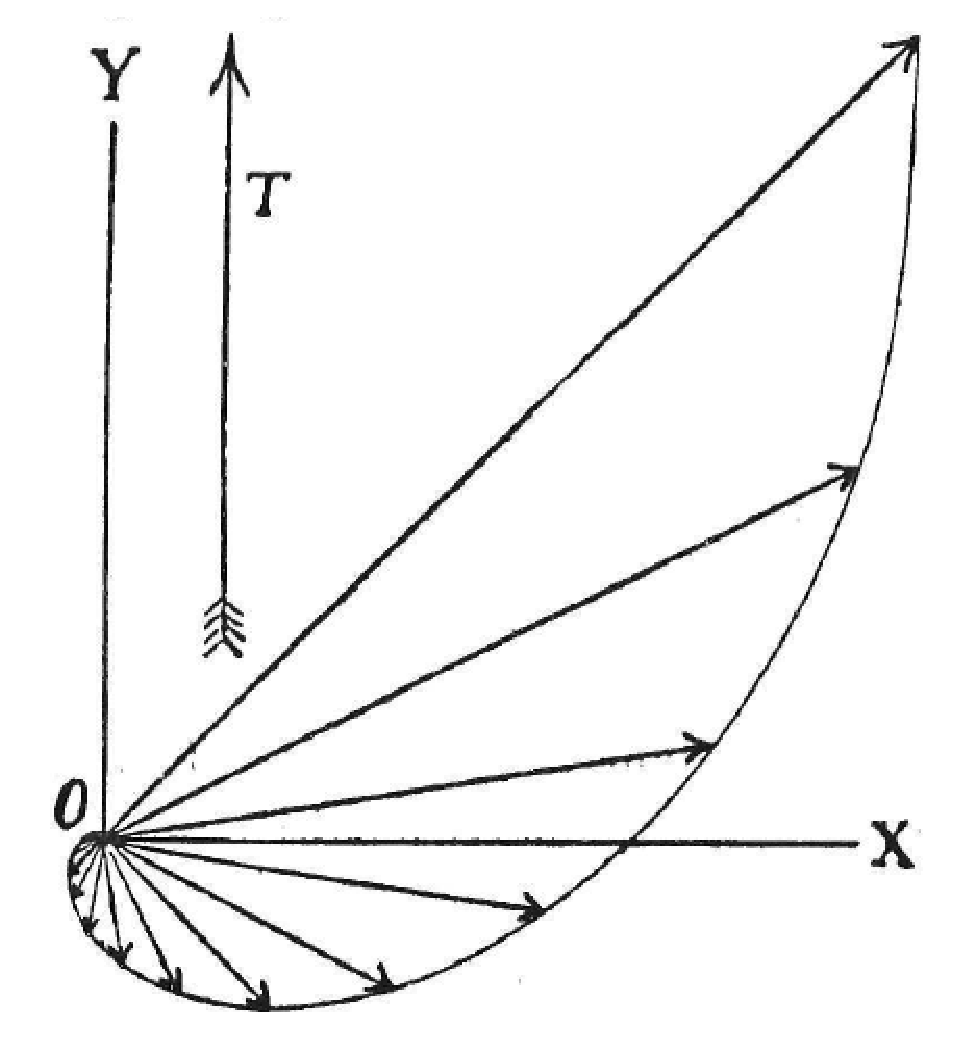
\includegraphics[width=5cm]{Ekman.eps}
		\caption*{} 
	\end{figure}
	\paragraph{水平体积输运}~{}\\
	体积输运:
	\[
	\begin{aligned}
	S &= \int_0^\infty  W dz \\
	&= {{{\tau _y}} \over {\sqrt 2 a\rho {A_z}}}{e^{i{\pi  \over 4}}}\int_0^\infty  {{e^{ - {\pi  \over {{D_0}}}(1 + i)z}}} dz\\
	&= {{{\tau _y}} \over {\sqrt 2 a\rho {A_z}}}{e^{i{\pi  \over 4}}}\left[ { - {{{D_0}} \over \pi }{1 \over {(1 + i)}}} \right]\left. {{e^{ - {\pi  \over {{D_0}}}(1 + i)z}}} \right|_0^\infty\\
	&= {{{\tau _y}} \over {2\Omega \sin \varphi \rho }} = {{{\tau _y}} \over {f\rho }}
	\end{aligned}
	\]
	\indent
    可以发现,得到的输运结果只有实部,没有虚部,说明体积输运方向为$x$轴正向,即在北半球水体向风向右侧90$\degree$输运.
    \subsubsection{有限深海漂流}
    \paragraph{假定}~{} \\
	有限深海Ekman漂流中用到了以下假定:\\
	\indent
	1) 海区无限广阔、有限深,远离海岸.\\
	\indent
	即无侧边界效应,仅有垂直湍流所生水平湍流摩擦力,并假定垂直湍流粘滞系数$A_z$为常量.由于海洋有限深,$z\rightarrow h,\vec{V}=0$\\
	\indent
	2) 定常均匀风场长时间作用.\\
	\indent
	即运动的基本参量与时间和水平坐标无关且海面无升降、无水平压强梯度.\\
	\indent
	3) 密度分布均匀,$\rho$为常数,不考虑热盐性质.\\
	\indent
    4) 采用$f$平面近似.\\
    控制方程和边界条件:
    \[
        \left\{
        \begin{aligned}
            &0=f v+A_{z} \frac{\partial^{2} u}{\partial z^{2}} \\
            &0=-f u+A_{z} \frac{\partial^{2} v}{\partial z^{2}}\\
            &\frac{\partial u}{\partial x}+\frac{\partial v}{\partial y}+\frac{\partial w}{\partial z}=0\\
            &z=0: \rho A_z\frac{\partial u}{\partial z}=0,\rho A_z\frac{\partial v}{\partial z}=-\tau_y\\
            &z\rightarrow h:u=v=0
        \end{aligned}
        \right.
    \]
    \paragraph{方程求解}~{}
    令$\xi=h-z$,定解问题化为:
    \begin{numcases}{}
        -fv=A_z\frac{\partial^2 u}{\partial \xi^2}\\
        fu=A_z\frac{\partial^2 v}{\partial \xi^2}\\
        \xi=h:\rho A_z\frac{\partial u}{\partial \xi}=0,\rho A_z\frac{\partial v}{\partial \xi}=\tau_y \nonumber\\
        \xi\rightarrow 0:u=v=0\nonumber
    \end{numcases}
    令$W=u+iv,\tau=\tau_x+i\tau_y$,控制方程:
    \[
        (11)+(12)\times i\Leftrightarrow \frac{d^{2} W}{d \xi^{2}}-j^{2} W=0
    \]
    边界条件:
    \[
        \begin{aligned}
            &\xi=h:\rho A_z\frac{\partial W}{\partial \xi}=\tau\\
            &\xi=0:W=0
        \end{aligned}
    \]
    与无限深海漂流解法类似,解得:
    \[
        W=\frac{(1+i) \tau_{y}}{2 a \rho A_{z}} \frac{s h(1+i) a \xi}{c h(1+i) a h}
    \]
    \paragraph{物理性质}~{}
    \paragraph{与水深的关系}~{}\\
    (1) $h≥2D_0$时,有限深海漂流流速流向与无限深海相同;
    (2) 水深越浅,流向随深度增加右偏(北半球)越缓慢;
    (3) 从上层到下层的流速矢量越是趋近风矢量的方向.
    \paragraph{体积输运}~{}\\
    (1) 在$x,y$方向(平行和垂直风向)都有输送;\\
    (2) 运输方向为风向右端,±90°之间:\\
        $$\displaystyle S_x>0;\\0<h<D_0,ah<\pi,S_y>0;D_0<h<2D_0,\pi<ah<2\pi,S_y<0;h>2D_0,S_y=0$$
    \subsubsection{漂流分离}
    \paragraph{利用风速大小相等、方向相反的两次观测余流分离漂流}~{}\\
    $\divideontimes$余流=漂流+恒量常流
    \begin{figure}[H]
        \centering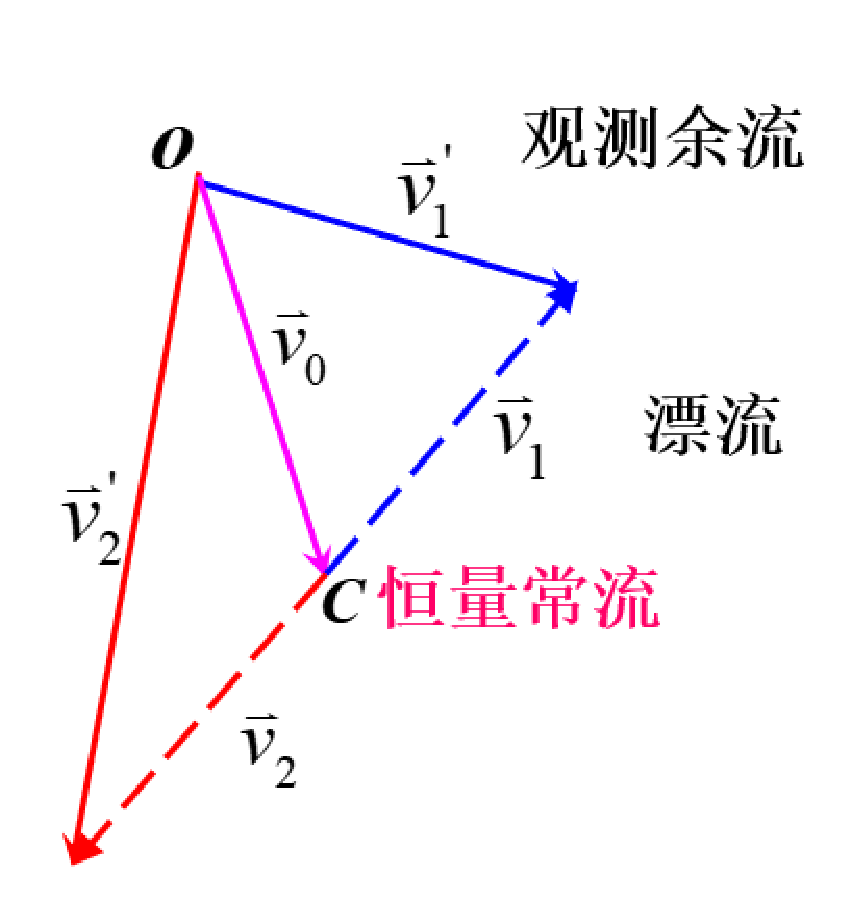
\includegraphics[width=5cm]{4.eps}
        \caption*{}
    \end{figure}
    \paragraph{利用一组风速大小相等、方向不同的实测余流分离漂流}~{}\\
    $\divideontimes$漂流速度矢量端点落在同一圆周上
    \begin{figure}[H]
        \centering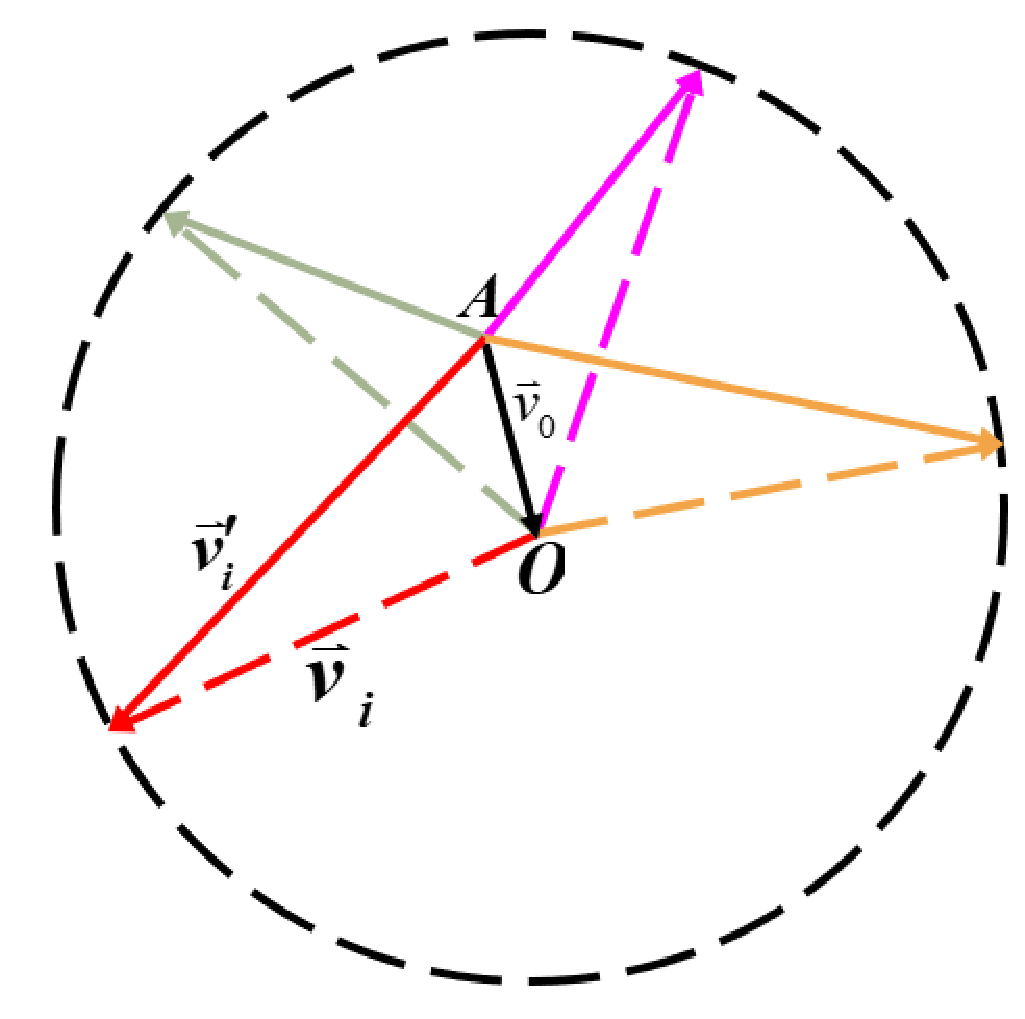
\includegraphics[width=5cm]{5.eps}
        \caption*{}
    \end{figure}
    \subsubsection{升降流}
    由不均匀风场或风场和地形配合产生的“较强烈”的铅直向流动。
    \paragraph{物理背景}~{}\\
    $\boxed{\mbox{非均匀风场}}\Rightarrow\boxed{\mbox{非均匀Ekman漂流}}\Rightarrow\boxed{\mbox{非均匀体积输运}}\Rightarrow\boxed{\mbox{辐聚辐散}}\mathop{\Rightarrow}\limits^{连续性}\boxed{\mbox{升降流}}$
    \begin{figure}[H]
        \centering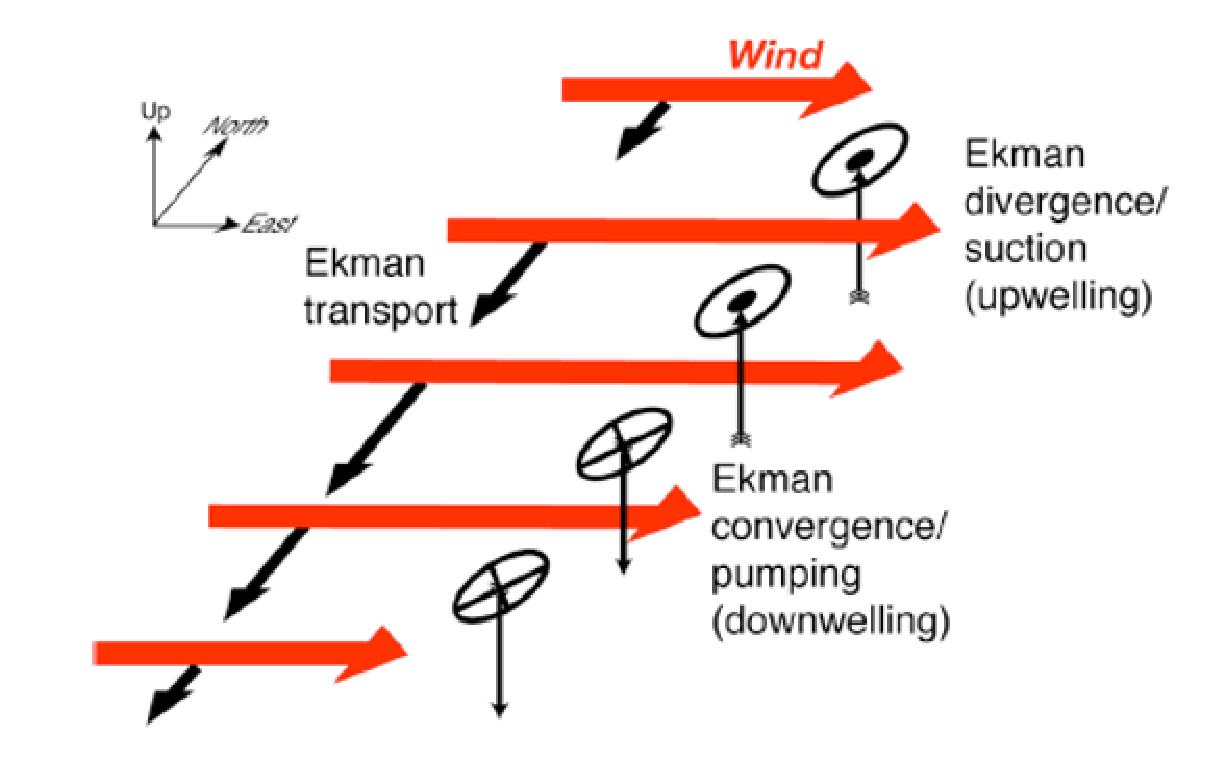
\includegraphics[width=8cm]{6.eps}
        \caption*{}
    \end{figure}
    \paragraph{赤道附近的升降流}~{} \\
    \begin{figure}[H]
        \centering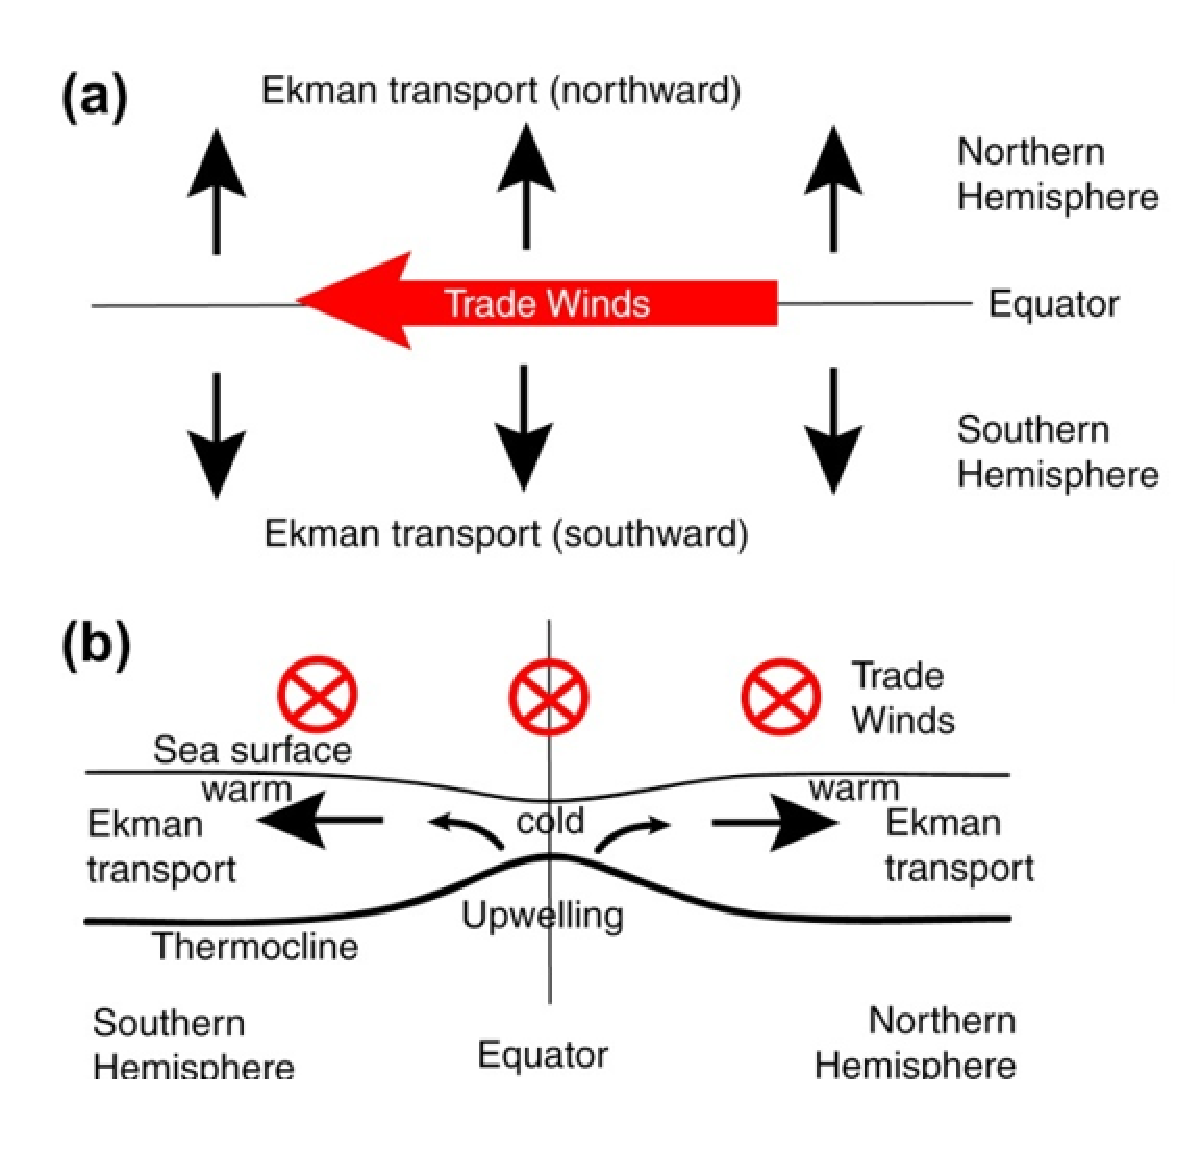
\includegraphics[width=8cm]{7.eps}
        \caption*{}
    \end{figure}
    \paragraph{顺(沿)岸风产生的升降流}~{} \\
    \begin{figure}[H]
        \centering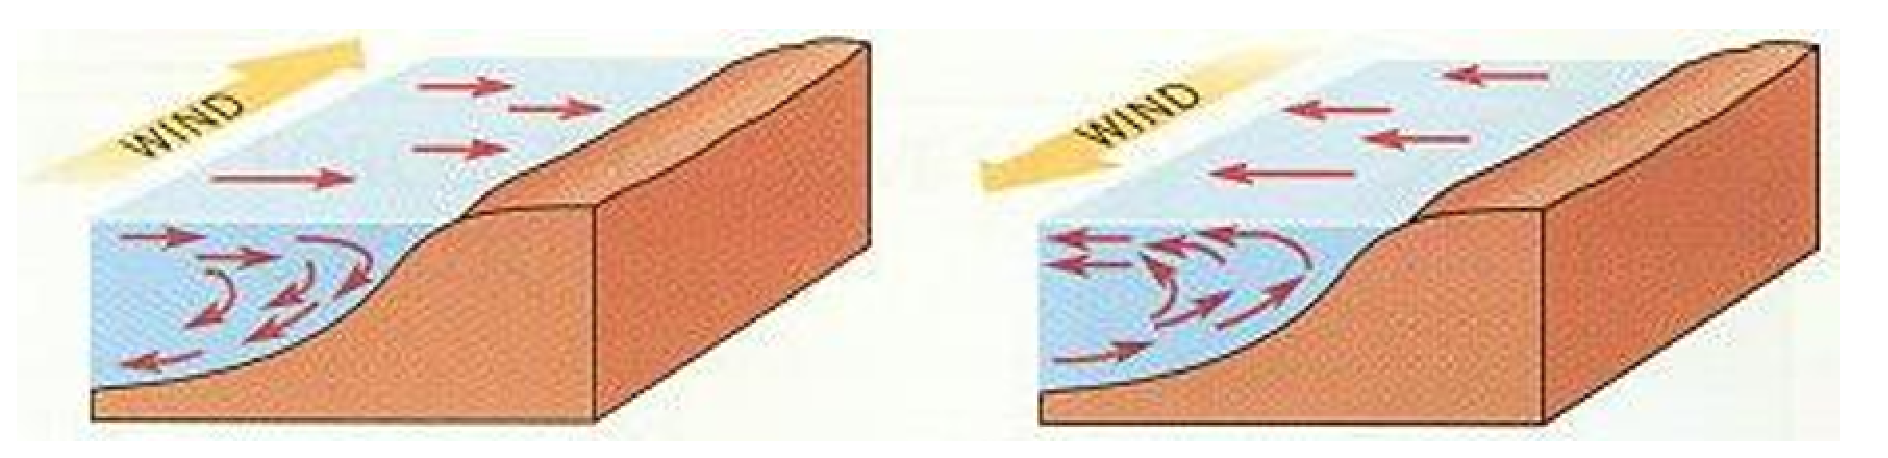
\includegraphics[width=10cm]{8.eps}
        \caption*{}
    \end{figure}
    \paragraph{气旋和反气旋产生的海洋升降流}~{} \\
    \begin{figure}[H]
        \centering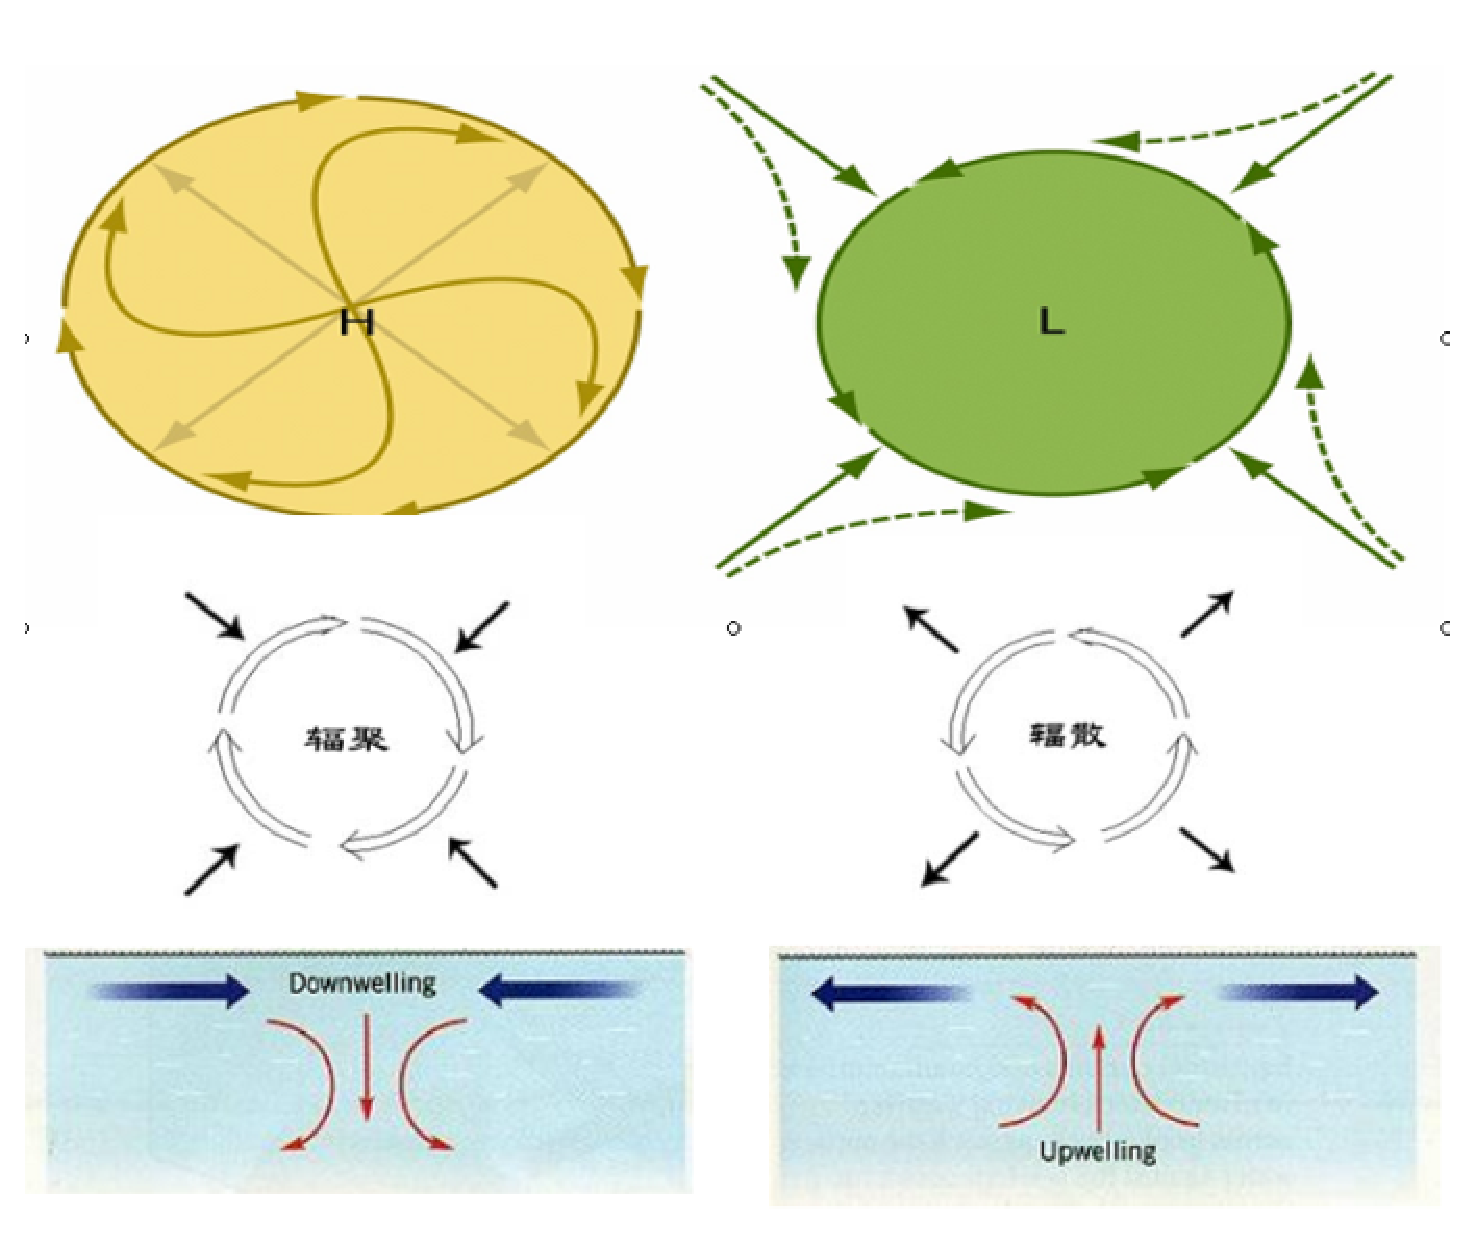
\includegraphics[width=8cm]{9.eps}
        \caption*{}
    \end{figure}
    \paragraph{假定}~{}\\
    (1) $\rho$为常数;\\
    (2) 直线风系,风仅沿$x$方向有变化;风区内为恒定的均匀风场;风区外无风;$\displaystyle \frac{\partial }{\partial y}=0$\\
    (3) 定常风场;$\displaystyle \frac{\partial }{\partial t}=0$\\
    (4) 大尺度;$Ro\ll 1$\\
    (5) 有限深度.$h \geq 2D_0$
    \paragraph{控制方程及边界条件}~{}
    \[
        \left\{
        \begin{aligned}
            &A_{l} \frac{\partial^{2} u}{\partial x^{2}}+A_{z} \frac{\partial^{2} u}{\partial z^{2}}+f v+g \frac{\partial \zeta}{\partial x}=0\\
            &A_{l} \frac{\partial^{2} v}{\partial x^{2}}+A_{z} \frac{\partial^{2} v}{\partial z^{2}}-f u=0\\
            &\frac{\partial u}{\partial x}+\frac{\partial w}{\partial z}=0
        \end{aligned}
        \right.
    \]
    \[
        \left\{
        \begin{aligned}
            &z=\zeta:\rho A_{z} \frac{\partial u}{\partial z}=0, \quad \rho A_{z} \frac{\partial v}{\partial z}=-\tau_{y} \quad(0 \leq x \leq L)\\
            &z=h:u=v=0\\
            &x=0:u=v=0\\
            &x\rightarrow\infty:u=v=0,\frac{\partial \zeta}{\partial x}=0
        \end{aligned}
        \right.
    \]
    \paragraph{结果讨论}~{}
    \begin{figure}[H]
        \centering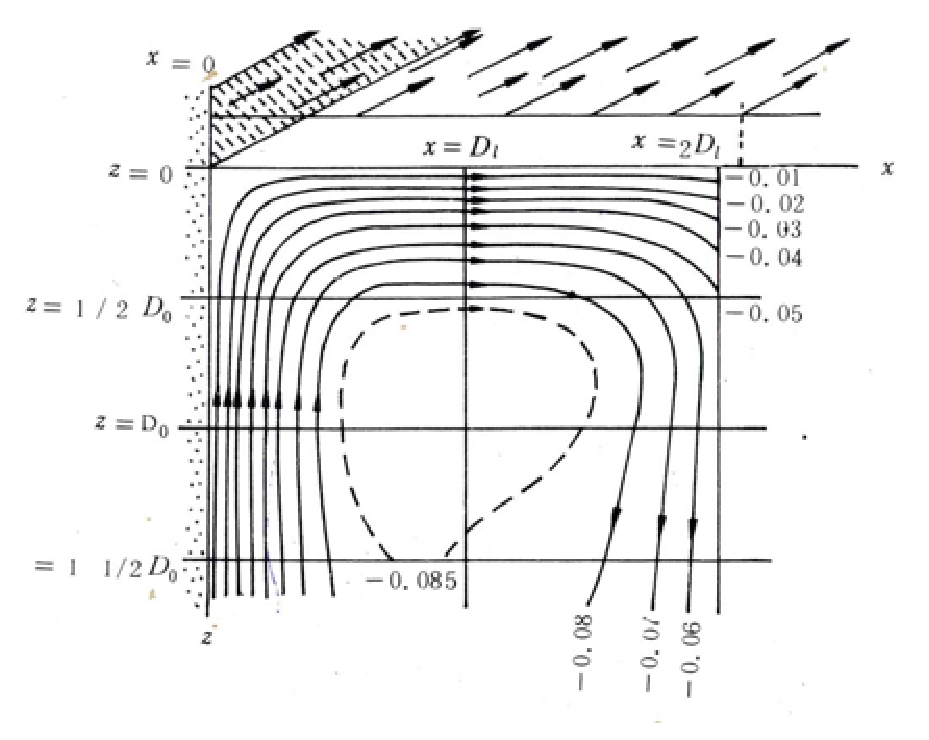
\includegraphics[width=8cm]{10.eps}
        \caption*{}
    \end{figure}
    (1) 近岸产生上升流$x\leq 0.5D_l$;\\
    (2) 风区外延附近下降流$x=2D_l$;\\
    (3) 上升流来自 $z=1.5D_0$或更深;\\
    (4) 最大$w$出现在$z=D_0$;\\
    (5) 上层离岸流,下层向岸流,构成一个循环.\\
    若风向与海岸成$\theta$角:\\
    \begin{figure}[H]
        \centering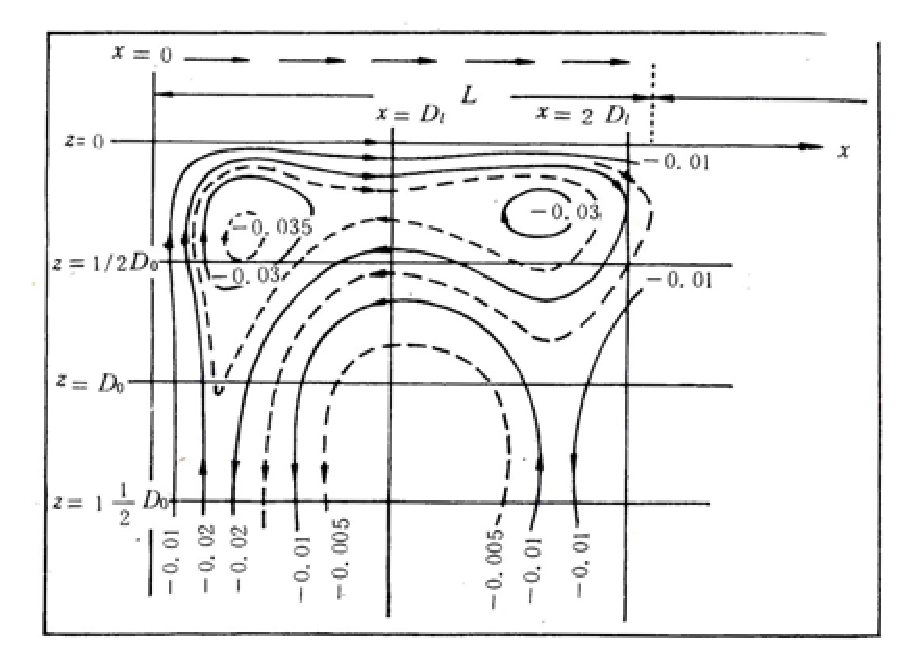
\includegraphics[width=8cm]{11.eps}
        \caption*{}
    \end{figure}
    (1) 三个升降流系统:两个顺时针,一个逆时针;\\
    (2) 大顺时针循环;\\
    (3) $\theta=21.5°$时,升降流达最大强度;\\
    (4) 纬度越低,升降流越强.
    \subsection{非定常运动}
    \subsubsection{漂流的发展}
    \paragraph{假定}~{} \\
    (1) 远离海岸和海底的开阔大洋;\\
    (2) 风场均匀恒定;\\
    (3) $\rho$为常数;\\
    (4) 海面无倾斜;\\
    (5) 运动非定常.\\
    \paragraph{控制方程}~{}
    \[
        \left\{
        \begin{aligned}
            &\frac{\partial u}{\partial t}-f v=A_{z} \frac{\partial^{2} u}{\partial z^{2}}\\
            &\frac{\partial v}{\partial t}+f u=A_{z} \frac{\partial^{2} v}{\partial z^{2}}
        \end{aligned}
        \right.
    \]
    \paragraph{初边值条件}~{}
    \[
        \left\{
        \begin{aligned}
            &z=0:A_z\frac{\partial u}{\partial z}=0,\rho A_z\frac{\partial v}{\partial z}=-\tau_y(t>0)\\
            &z\rightarrow\infty:u=v=0\\
            &t=0:u=v=0/u=C_1,v=C_2
        \end{aligned}
        \right.
    \]
    \paragraph{解的讨论}~{}
    \[
        \left\{
        \begin{aligned}
            &u=\frac{2 \pi \tau_{y}}{\rho f D_{0}} \int_{0}^{t^{\prime}} \frac{\sin (2 \pi \eta)}{\sqrt{\eta}} e^{\frac{\pi z^2}{4 D_{0}^{2}}} d \eta \\
            &v=\frac{2 \pi \tau_{y}}{\rho f D_{0}} \int_{0}^{t^{\prime}} \frac{\cos (2 \pi \eta)}{\sqrt{\eta}} e^{\frac{\pi z^2}{4 D_{0}^{2}}} d \eta
        \end{aligned}
        \right.
    \]
    根据下图\cite{Ekman}:
    \begin{figure}[H]
        \centering 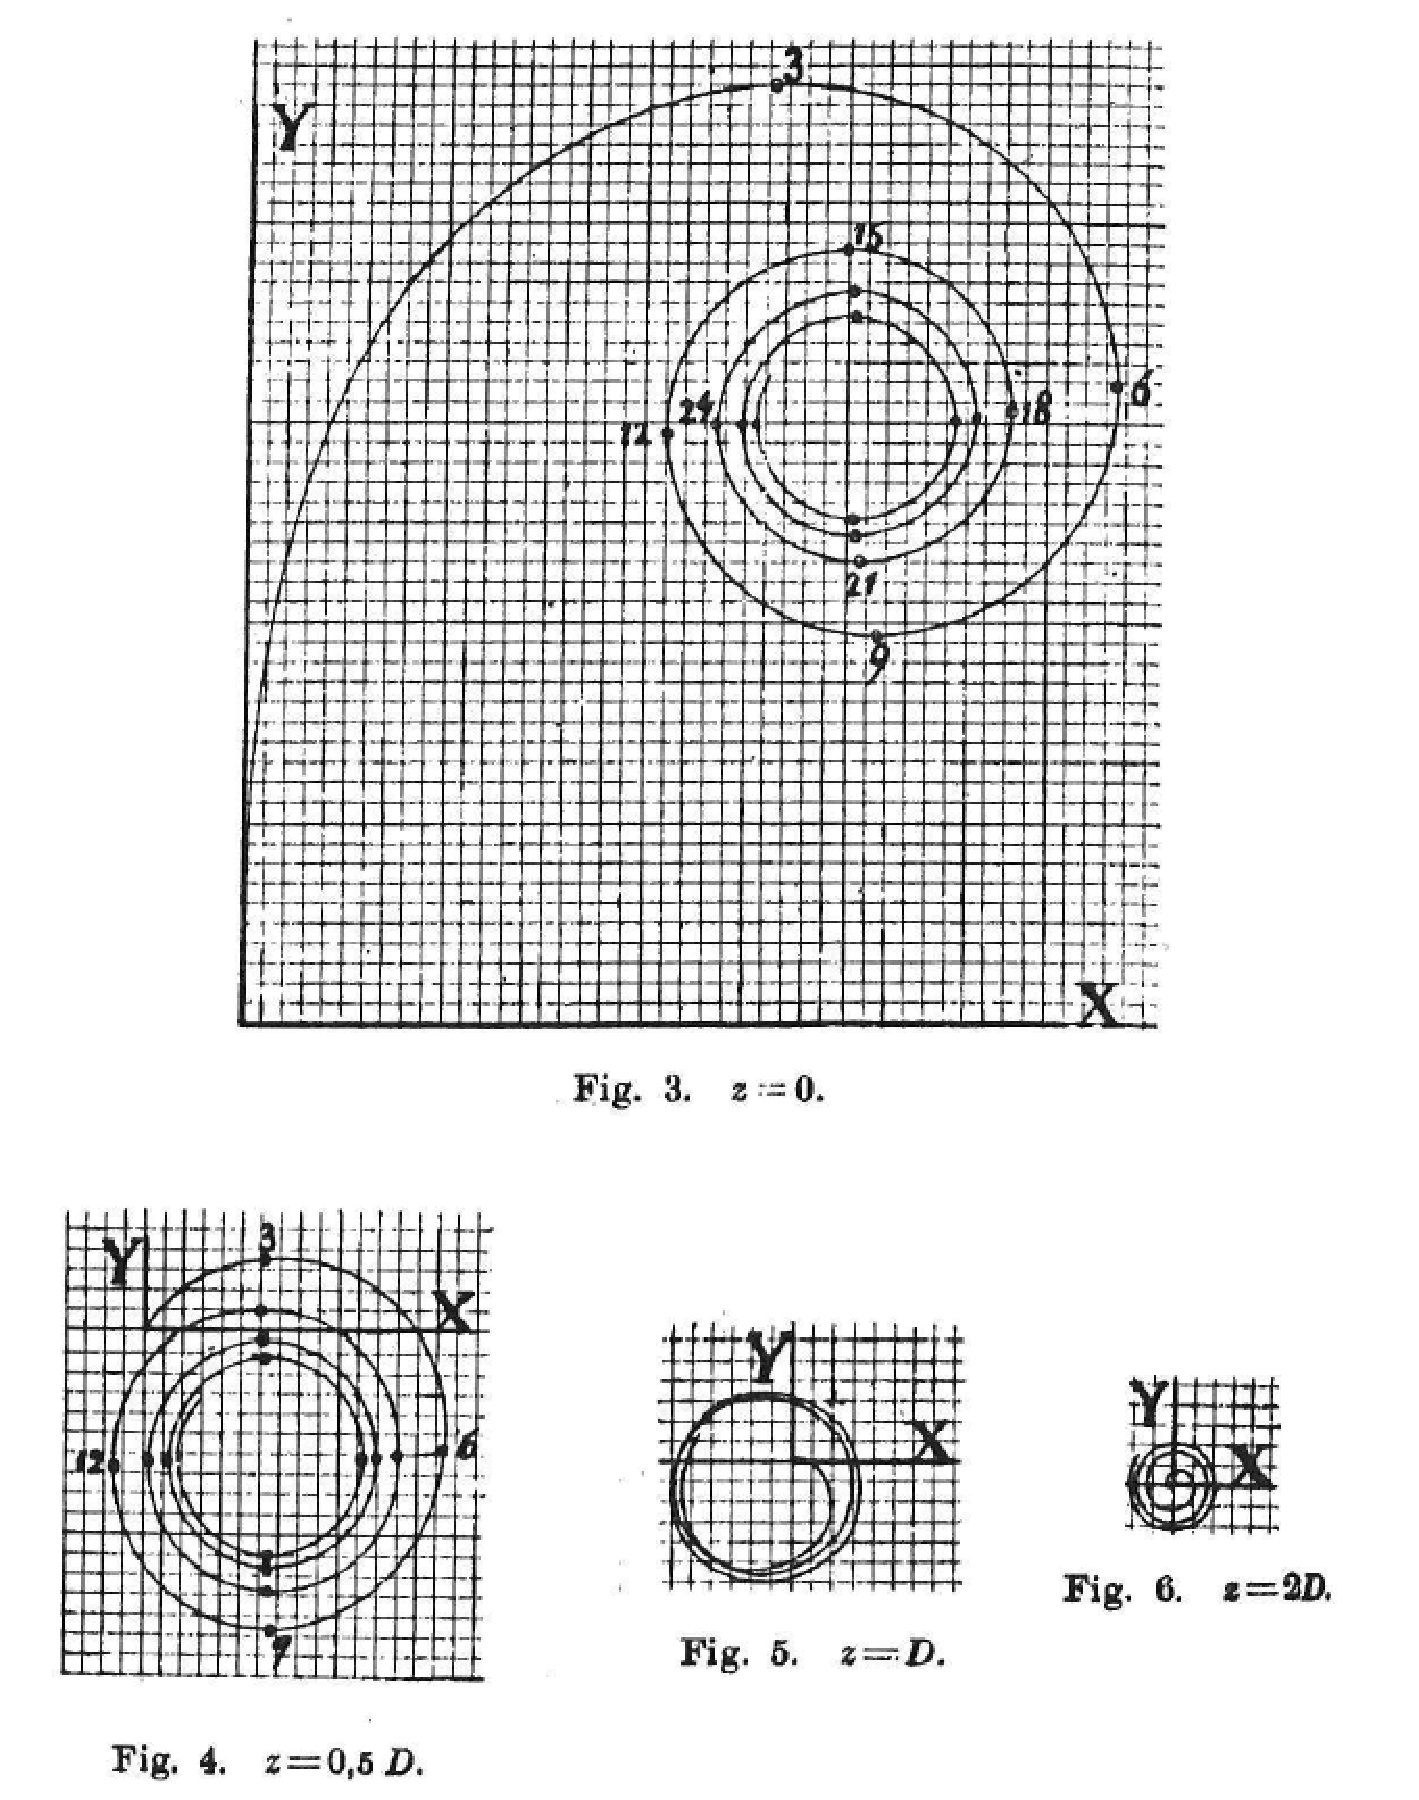
\includegraphics[width=7cm]{12.eps}
        \caption*{}
    \end{figure}
    随时间增加,空间某点流苏端点顺时针旋转(北半球),逐渐趋向一个极限值(即漂流).
    \subsubsection{惯性流}
    \paragraph{假定和方程}~{} \\
    (1) 风场消失或者流动离开风区;\\
    (2) 外部驱动小时,湍摩擦失去作用;\\
    (3) 流动转为由惯性项维持平衡;\\
    (4) 强制流动转变为自由流动.\\
    \begin{numcases}{}
        \frac{du}{dt}-fv=0 \label{ic1}\\
        \frac{dv}{dt}+fu=0 \label{ic2}
    \end{numcases}
    \paragraph{求解}~{}
    \[
        \begin{aligned}
            (\ref{ic1})\times u+(\ref{ic2}\times v)&\Leftrightarrow u \frac{d u}{d t}+v \frac{d v}{d t}=\frac{1}{2} \frac{d u^{2}}{d t}+\frac{1}{2} \frac{d v^{2}}{d t}=0 \\
            &\Leftrightarrow \frac{d}{d t}\left(u^{2}+v^{2}\right)=0\\
            &\Leftrightarrow u^{2}+v^{2}=c=V_{0}^{2}
        \end{aligned}
    \]
    \[
        \begin{aligned}
            (\ref{ic1}),(\ref{ic2})
            &\Rightarrow
            \left\{\begin{aligned}&v=\frac{d y}{d t}=\frac{1}{f} \frac{d u}{d t}\\ &u=\frac{d x}{d t}=\frac{1}{f} \frac{d v}{d t}\end{aligned}\right.\\
            &\Rightarrow
            \left\{\begin{aligned}&y-y^{\prime}=\frac{1}{f}\left(u-u^{\prime}\right)\\ &x-x^{\prime}=-\frac{1}{f}\left(v-v^{\prime}\right)\end{aligned}\right.\\
            &\Rightarrow
            \left\{\begin{aligned}&y-\left(y^{\prime}-\frac{u^{\prime}}{f}\right)=\frac{u}{f}\\ &x-\left(x^{\prime}+\frac{v^{\prime}}{f}\right)=-\frac{v}{f}\end{aligned}\right.\\
            &\Rightarrow\boxed{\left(y-y_{0}\right)^{2}+\left(x-x_{0}\right)^{2}=\frac{1}{f^{2}}\left(u^{2}+v^{2}\right)=\frac{V^{2}}{f^{2}}=r^{2}}
        \end{aligned}
    \]
    流体质点沿半径为$r$的圆周作匀速运动,这个圆称之为惯性圆,对应的流动为惯性流.
    \paragraph{惯性圆半径}~{}\\
    科氏力充当向心力:$\displaystyle \frac{V_0^2}{r}=fV_0\Rightarrow V_0=fr\Rightarrow r=\frac{V_0}{f}=\frac{V_0}{2\omega \sin \varphi}$\\
    随纬度增加而减小;赤道$r\rightarrow\infty$,水质点作直线运动.
    \paragraph{周期}~{}
     \[
        T_{i}=\frac{2 \pi r}{V_{0}}=\frac{2 \pi r}{f r}=\frac{2 \pi}{f}=\frac{\pi}{\omega \sin \varphi}
     \]
     \paragraph{运动方向}~{}\\
     北半球,顺时针;南半球,逆时针.
    \paragraph{背景流}~{}\\
    (1) 当无其他外加流动时,所有惯性圆的圆心位于同一条铅直线上,因而海水就像以角速度$2\omega \sin \varphi$旋转的刚体一样;\\
    (2) 当有其他外加流动时,除了在同一水平面上所有海水质点皆在同一时刻由同一流速速率外,还依外加流动速度方向移动.
    \newpage
    \subsection{风生大洋环流}
    \subsubsection{Sverdrup理论}
    \paragraph{假定}~{}\\
    (1) 远离海岸的大洋中部海区,Ro$\ll 1$大尺度、等深大洋$h$为常数;\\
    (2) 远离边界、无侧边界影响,无水平湍摩擦应力E$_l\ll 1$;\\
    (3) 定常风 定常流动;\\
    (4) $\rho$为常数;\\
    (5) $\beta$平面近似.\\
    \paragraph{控制方程}~{}
    \[
        \left\{
            \begin{aligned}
                &-f v=-\frac{1}{\rho} \frac{\partial p}{\partial x}+A_{z} \frac{\partial^{2} u}{\partial^{2} z} \\
                &fu=-\frac{1}{\rho} \frac{\partial p}{\partial y}+A_{z} \frac{\partial^{2} v}{\partial^{2} z} \\
                &0=-\frac{1}{\rho} \frac{\partial p}{\partial z}-g\\
                &\frac{\partial u}{\partial x}+\frac{\partial v}{\partial y}+\frac{\partial w}{\partial z}=0
            \end{aligned}
        \right.
    \]
    \paragraph{边界条件}~{}
    \[
        \left\{
            \begin{aligned}
                &z=\zeta(\mbox{海面}):\rho A_z\frac{\partial u}{\partial z}=\tau_{x\zeta},\rho A_z\frac{\partial v}{\partial z}=\tau_{y\zeta}\\
                &z=-h(\mbox{足够深}):u=v=0,\frac{\partial u}{\partial z}=\frac{\partial v}{\partial z}=0,\frac{\partial p}{\partial x} =\frac{\partial p}{\partial y}=0
            \end{aligned}
        \right.
    \]
    \paragraph{求解}~{}\\
    对上式进行垂直积分:
    \begin{numcases}{}
        -fM_y=-\frac{\partial P}{\partial x}+\tau_{x\zeta}\\
        fM_x=-\frac{\partial P}{\partial y}+\tau_{y\zeta}\\
        \frac{\partial M_x}{\partial x}+\frac{\partial M_y}{\partial y}=0\nonumber
    \end{numcases}
    其中,$\displaystyle M_x=\int_{-h}^0\rho udz,M_y=\int_{-h}^0\rho vdz,P=\int_{-h}^0 pdz,\tau_{x\zeta}=\int_{-h}^0\rho A_z\frac{\partial^2 u}{\partial z^2}=\rho A_{z}\left(\left.\frac{\partial u}{\partial z}\right|_{z=0}-\left.\frac{\partial u}{\partial z}\right|_{z=-h}\right)\quad (\zeta\ll h)$
    \[
        \begin{aligned}
            \frac{\partial (1)}{\partial y}-\frac{\partial (2)}{\partial x}&\Leftrightarrow -M_y\frac{\partial f}{\partial y}\mathop{\boxed{-f\frac{\partial M_y}{\partial y}-f\frac{\partial M_x}{\partial x}}}\limits^{0}=\frac{\partial \tau_{x\zeta}}{\partial y}-\frac{\partial \tau_{y\zeta}}{\partial x}\\
            &\Leftrightarrow M_{y} \frac{\partial f}{\partial y}=\frac{\partial \tau_{y \zeta}}{\partial x}-\frac{\partial \tau_{x \zeta}}{\partial y}\\
            &\Leftrightarrow\mathop{\boxed{\color{red}\beta M_y=\operatorname{rot}_z\tau_\zeta}}\limits_{\mbox{Sverdrup方程}}
        \end{aligned}
    \]
    $\color{red} \mbox{Sverdrup方程的物理意义1}$:海水南北向的输运由风应力旋度所驱动.
    \paragraph{讨论}~{}\\
    将质量输运分为Ekman漂流输运与地转流输运两部分:
    \[
        \begin{aligned}
            &M_x=M_{xE}(\mbox{Ekman漂流})+M_{xg}(\mbox{地转流})\\
            &M_y=M_{yE}(\mbox{Ekman漂流})+M_{yg}(\mbox{地转流})
        \end{aligned}
    \]
    \begin{numcases}{}
        -fM_{yE}=\tau_{x\zeta}\\
        fM_{xE}=\tau_{y\zeta}\\
        -fM_{yg}=-\frac{\partial P}{\partial x}\\
        fM_{yg}=-\frac{\partial P}{\partial y}
    \end{numcases}
    \begin{align}
        &\frac{\partial(17)}{\partial y}-\frac{\partial(18)}{\partial x}\Leftrightarrow\frac{\partial {M}_{xE}}{\partial x}+\frac{\partial {M}_{yE}}{\partial y}=\boxed{\nabla \cdot \vec{{M}}_{E}=\left(\operatorname{rot}_{z} \vec{\tau}_{\zeta}-{\beta} {M}_{y E}\right) / {f}}\\
        &\frac{\partial(19)}{\partial y}-\frac{\partial(20)}{\partial x}\Leftrightarrow\frac{\partial {M}_{xg}}{\partial x}+\frac{\partial {M}_{yg}}{\partial y}=\boxed{\nabla \cdot \vec{{M}}_{g}=-\beta M_{yg}/f}
    \end{align}
    (1) Ekman漂流质量输运的水平散度与$\circled{1}$风应力旋度$\circled{2} f\circled{3} \beta$有关.\\
    (2) 地转流质量输运的水平辐散引起南北向的地转运动.
    \[
        (21)+(22)\Leftrightarrow \operatorname{rot}_z\vec{tau}_\zeta-\beta M_y=0\Leftrightarrow\boxed{\color{red} \beta M_y=\operatorname{rot}_z\vec{\tau}_\zeta}
    \]
    $\color{red} \mbox{Sverdrup方程的物理意义2}$:地转流流量的散度和Ekman漂流流量的散度相平衡,所以Sverdrup方程又称Sverdrup平衡.\\
    (1) 所有南北向的地转运动,必须显示水平散度;\\
    (2) 虽然Ekman漂流流量的散度与地转流流量的散度本身不为0,但是它们的和,即总流量的水平散度必须为0,说明Ekman漂流流量的散度和地转流流量的散度刚好取得平衡;\\
    (3) $\operatorname{rot}_z\vec{\tau}_\zeta=0$:只存在东西方向的输运,$\operatorname{rot}_z\vec{\tau}_\zeta>0$:质量输运向北(北半球),$\operatorname{rot}_z\vec{\tau}_\zeta<0$:质量输运向南(南半球);\\
    (4) 地转流引起的南北质量运输量比Ekman漂流引起的大.
    \paragraph{缺陷}~{}\\
    设仅有纬向风,且$\tau_{x\zeta}$仅为$y$的函数:
    \[
        M_y=\frac{1}{\beta}\operatorname{rot}_z\vec{\tau}_\zeta=\frac{1}{\beta}\left(\cancel{\frac{\partial \tau_{y\zeta}}{\partial x}}-\frac{\partial \tau_{x\zeta}}{\partial y}\right)=-\frac{a}{2\omega\cos\varphi}\frac{\partial\tau_{x\zeta}}{\partial y}
    \]
    \[
        \frac{\partial M_{x}}{\partial x}=-\frac{\partial M_{y}}{\partial y}\Rightarrow M_{x}=\frac{x}{2 \omega \cos \varphi}\left(a \frac{\partial^{2} \tau_{x f}}{\partial y^{2}}+\frac{\partial \tau_{x f}}{\partial y} t g \varphi\right)+{\color{red}c(y)}
    \]
    在东、西边界,$M_x=0$而Sverdrup理论不能同时满足.
    \subsubsection{Stommel理论}
    \paragraph{假定}~{}\\
    (1) 远离海岸的大洋中部海区,Ro$\ll 1$大尺度、等深大洋$h$为常数;\\
    (2) 远离边界、无侧边界影响,无水平湍摩擦应力E$_l\ll 1$;\\
    (3) 定常风 定常流动;\\
    (4) $\rho$为常数;\\
    (5) $\beta$平面近似;\\
    $\mbox{(6) 考虑底摩擦}$
    \paragraph{控制方程}~{}
    \[
        \left\{
            \begin{aligned}
                &-f v=-g \frac{\partial \zeta}{\partial x}+A_{z} \frac{\partial^{2} u}{\partial^{2} z} \\
                &fu=-g \frac{\partial \zeta}{\partial y}+A_{z} \frac{\partial^{2} v}{\partial^{2} z} \\
                &0=-\frac{1}{\rho} \frac{\partial p}{\partial z}-g\\
                &\frac{\partial u}{\partial x}+\frac{\partial v}{\partial y}+\frac{\partial w}{\partial z}=0
            \end{aligned}
        \right.
    \]
    \paragraph{边界条件}~{}
    \[
        \left\{
            \begin{aligned}
                &z=\zeta(\mbox{海面}):\tau_{x , \zeta}=\left.\rho A_{z} \frac{\partial u}{\partial z}\right|_{t=\zeta}=-F \cos (\pi y / b),\tau_{x , \zeta}=0\\
                &z=-h(\mbox{海底}):\tau_{x,-h}=\rho+\left.\frac{\partial u}{\partial z}\right|_{t=-h}={\color{red}\rho k u},\tau_{y,-h}=\rho+\left.\frac{\partial v}{\partial z}\right|_{t=-h}={\color{red}\rho k v}
            \end{aligned}
        \right.
    \]
    \paragraph{求解}~{}\\
    对上式进行垂直平均:
    \[
        \left\{
        \begin{aligned}
            &-f\left\langle v\right\rangle=-g \frac{\partial \zeta}{\partial x}+\left.\frac{A_{z}}{h+\zeta} \frac{\partial u}{\partial z}\right|_{\zeta}-\left.\frac{A_z}{h+\zeta} \frac{\partial u}{\partial z}\right|_{-h}\\
            &f\left\langle u\right\rangle=-g \frac{\partial \zeta}{\partial y}+\left.\frac{A_{z}}{h+\zeta} \frac{\partial v}{\partial z}\right|_{\zeta}-\left.\frac{A_z}{h+\zeta} \frac{\partial v}{\partial z}\right|_{-h}\\
            &\frac{\partial}{\partial x}\left[\left(n+\zeta\right)\left\langle u\right\rangle\right]+\frac{\partial}{\partial y}[(n+\zeta)\left\langle v\right\rangle]=0
        \end{aligned}
        \right.
    \]
    
    将边界条件代入方程:
    \begin{numcases}{}
        0=f \rho h v-F \cos \left(\left. \pi y \middle/ b \right.\right)-\rho k u-\rho g h \frac{\partial \zeta}{\partial x} \quad(\zeta \ll k) \label{stm1}\\
        0=-f \rho h u-\rho k v-\rho g h \frac{\partial \zeta}{\partial y}\label{stm2}\\
        \frac{\partial u}{\partial x}+\frac{\partial v}{\partial y}=0 \nonumber
    \end{numcases}
    \[
        \frac{\partial (\ref{stm1})}{\partial y}-\frac{\partial (\ref{stm2})}{\partial x}\Rightarrow \frac{h}{k}[\beta v+r \sin (\pi y / b)]+{\color{red}\overbrace{\left(\frac{\partial v}{\partial x}-\frac{\partial u}{\partial y}\right)}^{\color{red}\mbox{来源于底摩擦}}}=0
    \]
    引入流函数$\displaystyle \psi:u=\frac{\partial \psi}{\partial y},v=-\frac{\partial \psi}{\partial x}$:
    \[
        {\color{red}\overbrace{\frac{\partial^{2} \psi}{\partial x^{2}}+\frac{\partial^{2} \psi}{\partial y^{2}}}^{\color{red}\mbox{来源于底摩擦}}}+\frac{h}{k} \beta \frac{\partial \psi}{\partial x}=\frac{h}{k} r \sin \frac{\pi y}{b}
    \]
    边界条件:
    \[
        \psi(0, y)=\psi(a, y)=\psi(x, 0)=\psi(x, b)=0
    \]
    \[
        \Rightarrow \psi(x, y)=\frac{F b}{k \pi} \sin \frac{\pi y}{b}\left[\frac{e^{\frac{h \beta}{2 k}(a-x)} \operatorname{sh} \alpha x+e^{\frac{h \beta}{2 k} x} \operatorname{sh} \alpha(a-x)}{\operatorname{sh} \alpha a}-1\right]
    \]
    特别地,若$\beta=0$:$\displaystyle\psi(x, y)=\frac{F b}{k \pi} \sin \frac{\pi y}{b}\left[\frac{\operatorname{sh} \frac{\pi}{b} x+\operatorname{sh} \frac{\pi}{b}(a-x)}{\operatorname{sh} \frac{\pi}{b} a}-1\right]$
    \paragraph{讨论}~{图片来自$Introduction \;to \; Physical \;Oceanography$(Robert H. Stewart,2008 pp190)}
    \begin{figure}[H]
        \centering 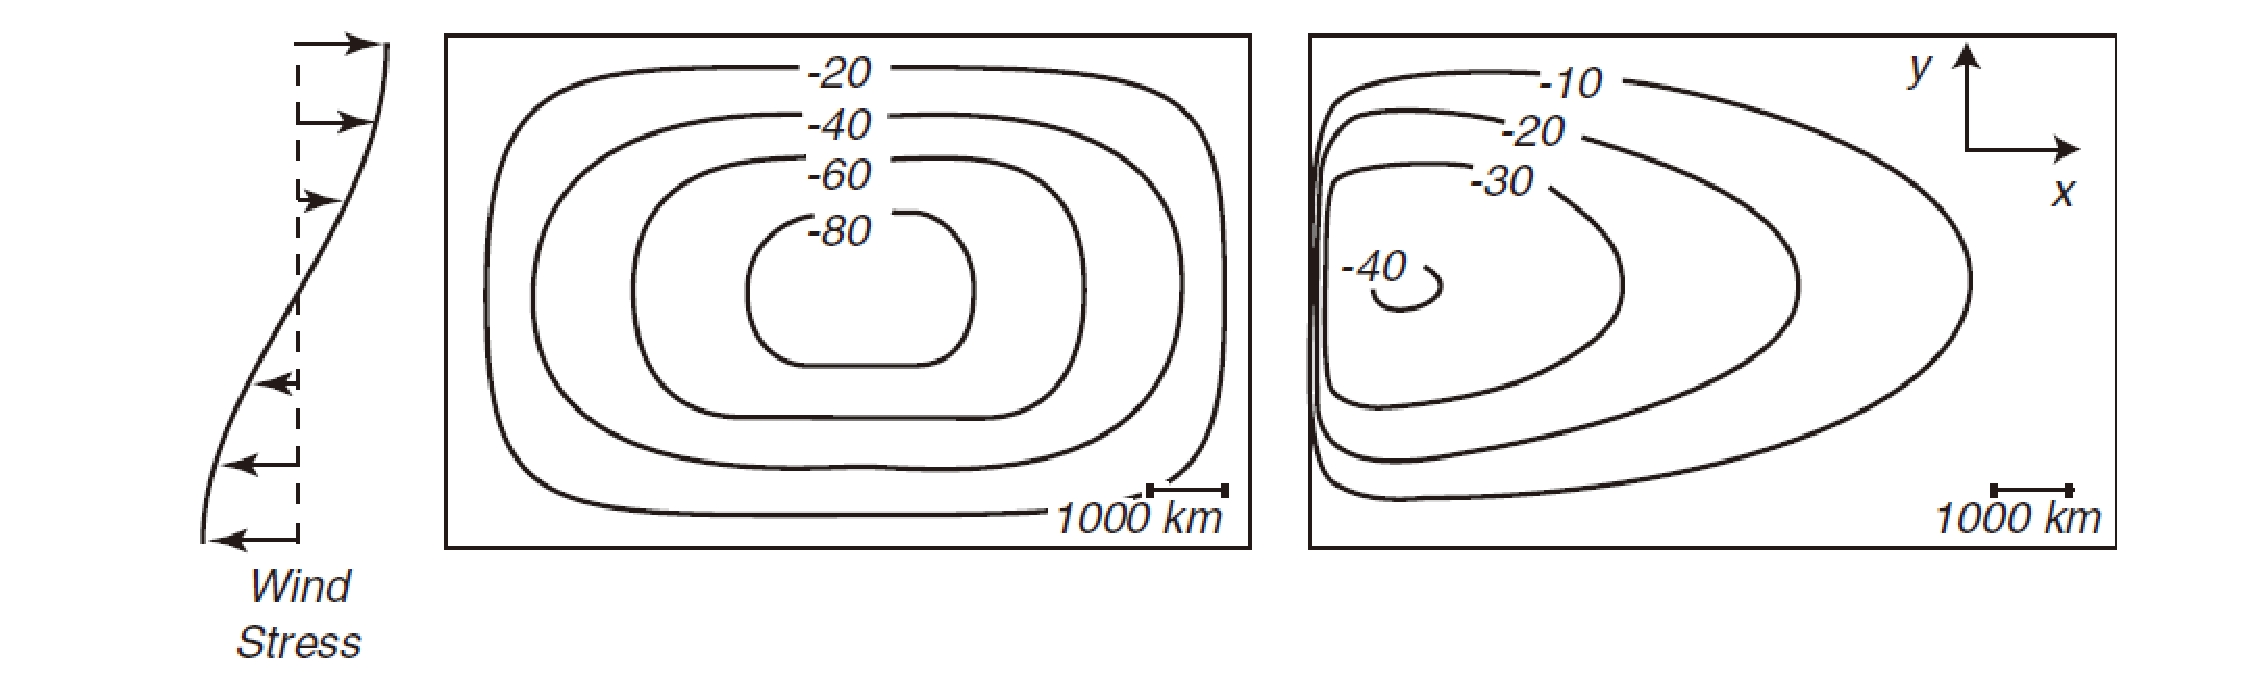
\includegraphics[width=18cm]{13.eps}
        \caption*{\large$  \color{red}\divideontimes\beta\mbox{效应导致了西向强化现象.}$}
    \end{figure}
    \begin{framed}
    \begin{multicols}{2}
        \begin{spacing}{0.8}
        \centering 
        $\mathbf\beta=0$(非旋转坐标系或f平面近似):\\
        (1) 流线南北对称;\\
        (2) 流线东西对称.\\
        $\mathbf\beta\neq 0$($\beta$平面近似):\\
        (1) 流线南北对称;\\
        (2) 流线东西不对称,西部密集,东部稀疏.
        \end{spacing}
    \end{multicols}
    \end{framed}
    \subsubsection{惯性理论}
    \paragraph{方程}~{}\\
    在Sverdrup理论的控制方程中引入惯性项:
    \[
        \left\{
            \begin{aligned}
                &\frac{du}{dt}-f v=-\frac{1}{\rho} \frac{\partial p}{\partial x}+A_{z} \frac{\partial^{2} u}{\partial^{2} z} \\
                &\frac{dv}{dt}+fu=-\frac{1}{\rho} \frac{\partial p}{\partial y}+A_{z} \frac{\partial^{2} v}{\partial^{2} z} \\
                &0=-\frac{1}{\rho} \frac{\partial p}{\partial z}-g\\
                &\frac{\partial u}{\partial x}+\frac{\partial v}{\partial y}+\frac{\partial w}{\partial z}=0
            \end{aligned}
        \right.
    \]
    \paragraph{求解}~{}
    \paragraph{内区(中部区)}~{}\\
    满足Sverdrup理论:$\displaystyle \beta M_y=\operatorname{rot}_z\tau_\zeta,M_y=\frac{\partial \varphi}{\partial x}=\frac{1}{\beta} \operatorname{rot}_{z} \tau_{\zeta}=\frac{1}{\beta}\left(\frac{\partial \tau_{y\zeta}}{\partial x}-\frac{\partial \tau_{x\zeta}}{\partial y}\right)$\\
    又设风应力:$\displaystyle \tau_{x\zeta}=-W\left(1-\frac{y^2}{s^2}\right),\tau_{y\zeta}=0\quad (0\leq y \leq s)$\\
    \[
        \begin{aligned}
            \Rightarrow &\frac{\partial \varphi}{\partial x}=-\frac{2W}{\beta s^2}y\\
            \Rightarrow &\varphi=-\frac{2W}{\beta s^2}yx+C(y)\\
            (x=r:\varphi=0)\quad &0=-\frac{2W}{\beta s^2}yr+C(y)\\
            \Rightarrow &\varphi=\frac{2W}{\beta s^2}y(r-x)
        \end{aligned}
    \]
    \paragraph{大洋西部海域}~{}\\
    不考虑湍摩擦效应:
    \begin{numcases}{}
        \frac{du}{dt}-f v=-\frac{1}{\rho} \frac{\partial p}{\partial x} \label{int1}\\
        \frac{dv}{dt}+fu=-\frac{1}{\rho} \frac{\partial p}{\partial y} \label{int2}\\
        0=-\frac{1}{\rho} \frac{\partial p}{\partial z}-g\nonumber\\
        \frac{\partial u}{\partial x}+\frac{\partial v}{\partial y}+\frac{\partial w}{\partial z}=0\nonumber
    \end{numcases}
    \begin{align}
            \frac{\partial (\ref{int2})}{\partial x}-\frac{\partial (\ref{int1})}{\partial y}           &\Leftrightarrow \frac{d}{d t}(\xi_r+f)+(\xi_r+f)\left(\frac{\partial u}{\partial x}+\frac{\partial v}{\partial y}\right)=0 \nonumber\\
            &\Leftrightarrow \frac{d}{d t}\left(\xi_{r}+f\right)=-\left(\xi_{r}+f\right)\left(\frac{\partial u}{\partial x}+\frac{\partial v}{\partial y}\right) \label{int3}
    \end{align}
    $\displaystyle \xi_r=\frac{\partial v}{\partial x}-\frac{\partial u}{\partial y}$相对涡度,$f$行星涡度,$\xi_a=\xi_r+f$绝对涡度.\\
    对连续方程进行垂向平均:
    \begin{align}
        &\frac{\partial \zeta}{\partial t}+\frac{\partial[(h+\zeta)\langle u\rangle]}{\partial x}+\frac{\partial[(h+\zeta)(v)]}{\partial y}=0\nonumber\\
        \Leftrightarrow & \frac{d(\zeta+h)}{d t}+(\zeta+h)\left(\frac{\partial(u)}{\partial x}+\frac{\partial(v)}{\partial y}\right)=0 \nonumber\\
        (\mbox{令}H=h+\zeta)\Leftrightarrow & \frac{d H}{d t}+H\left(\frac{\partial u}{\partial x}+\frac{\partial v}{\partial y}\right)=0 \label{int4}
    \end{align}
    将$(\ref{int4})$代入$(\ref{int3})$中:
    \begin{align}
         &\Rightarrow \frac{d}{d t}\left(\xi_{r}+f\right)=\frac{1}{H}\left(\xi_{r}+f\right) \frac{d H}{d t}\nonumber\\
         &\Rightarrow \frac{1}{H} \frac{d}{d t}(\xi_r+f)=\frac{1}{H^{2}}\left(\xi_{r}+f\right) \frac{d H}{d t}\nonumber\\
         &\Rightarrow {\color{red} \boxed{\frac{d}{d t}\left(\frac{\xi_{r}+f}{H}\right)=0}} \label{veq}
    \end{align}
    $(\ref{veq})$为$\color{red}\mbox{位势涡度守恒方程}$.\\
    假设在西边界区$\displaystyle\frac{\partial u}{\partial y}=0$,则:
    \[
        \xi_{r}=\frac{\partial v}{\partial x}-\frac{\partial u}{\partial y}=\frac{\partial v}{\partial x}=\frac{\partial}{\partial x}\left(\frac{1}{H} \frac{\partial \varphi}{\partial x}\right)
    \]
    代入$(\ref{veq})$:
    \[
        \begin{aligned}
            &\frac{d}{d t}\left[\frac{\frac{\partial}{\partial x}\left(\frac{1}{M} \frac{\partial \varphi}{\partial x}\right)+f}{H}\right]=0\\
            \Rightarrow & \frac{\frac{\partial}{\partial x}\left(\frac{1}{H} \frac{\partial \varphi}{\partial x}\right)+f}{H}=F(\varphi)\\
            \Rightarrow & \frac{1}{H} \frac{\partial^{2} \varphi}{\partial x^{2}}+f_{0}+\beta y=H F(\varphi)=G(\varphi)
        \end{aligned}
    \]
    \paragraph{在西边界层的边缘}~{}\\
    内部的解即为西边界的解,惯性项可以忽略:
    \[
        x=L:f_0+\beta y=G(\phi_i)
    \]
    \paragraph{在内区的边缘($L\ll r$)}~{}
    $$ \varphi_{i}=\frac{2 W}{\beta s^{2}} y(r-x)=\frac{2 W}{\beta s^{2}} y(r-L)=\frac{2 W}{\beta s^{2}} y r=u^* y\quad \left( u^*=\frac{2W}{\beta s^2}r\right)$$
    上面两解应该等价,因此:
    \[
        \begin{aligned}
            &f_0+\beta y=G(u^*y) \\
            \Rightarrow & G(\varphi)=f_0+\beta\frac{\varphi}{u^*}\\
            \Rightarrow & \frac{\partial^{2} \varphi}{\partial x^{2}}+H\left(f_{0}+\beta y\right)=H\left(f_{0}+\beta \frac{\varphi}{u^*}\right)\\
            \Rightarrow & \frac{\partial^{2} \varphi}{\partial x^{2}}-\frac{H \beta}{u^{*}} \varphi=-H \beta y
        \end{aligned}
    \]
    再结合两个边界条件:$\displaystyle x=0:\left\{\begin{aligned}&\varphi(0,y)=0\nonumber\\&\frac{\partial \varphi}{\partial x}=0\nonumber\end{aligned}\right.$,上面的二阶常系数线性微分方程的解为:
    \[
        \varphi=u^{*} y\left[1-e^{-\left(H \beta / u^*\right)^{1 / 2} x}\right]
    \]
    海水南北输运:
    \[
        \color{red}
        \boxed{
        M_y=\frac{\partial \varphi}{\partial x}=\left(u^* H\beta\right)^{1 / 2} {y} e^{-\left({H} \beta {u}^*\right)^{1/2}{x}}
        }
    \]
    在西边界区域有一强烈的北向流动,近岸处质量运输很大,随着离岸距离的增加,质量输运迅速减少.
    \subsubsection{Munk理论}
    \paragraph{假定}~{}\\
    (1) 矩形大洋$r\times 2s$;\\
    (2) 远离海岸的等深封闭矩形大洋,静止时水深为常量$h$;\\
    (3) $\color{red} \mbox{增加了侧向摩擦}$.
    \paragraph{控制方程}~{}
    \[
        \left\{
            \begin{aligned}
            &-fv=-\frac{1}{\rho} \frac{\partial p}{\partial x}+{\color{red}A_{l}\left(\frac{\partial^{2} u}{\partial x^{2}}+\frac{\partial^{2} u}{\partial y^{2}}\right)}+A_{z} \frac{\partial^{2} u}{\partial z^{2}}\\
            &fu=-\frac{1}{\rho} \frac{\partial p}{\partial y}+{\color{red}A_{l}\left(\frac{\partial^{2} v}{\partial x^{2}}+\frac{\partial^{2} v}{\partial y^{2}}\right)}+A_{z} \frac{\partial^{2} v}{\partial z^{2}}\\
            &0=-\frac{1}{\rho} \frac{\partial p}{\partial z}-g\\
            &\frac{\partial u}{\partial x}+\frac{\partial v}{\partial y}+\frac{\partial w}{\partial z}=0
        \end{aligned}
        \right.
    \]
    \paragraph{边界条件}~{}
    \[
        \left\{
        \begin{aligned}
            &z=\zeta, \quad \rho A_{z} \frac{\partial u}{\partial z}=\tau_{x \zeta}, \rho A_{z} \frac{\partial v}{\partial z}=\tau_{y \zeta}\\
            &z=-h, \quad u=v=0, \frac{\partial u}{\partial z}=\frac{\partial v}{\partial z}=0
        \end{aligned}
        \right.
    \]
    \paragraph{求解}~{}\\
    全流方程(垂直积分):
    \begin{numcases}{}
        -fM_y=-\frac{\partial P}{\partial x}+A_l\left(\frac{\partial^2 M_x}{\partial x^2}+\frac{\partial^2 M_x}{\partial y^2}\right)+\tau_{x\zeta}\label{mnk1}\\
        fM_x=-\frac{\partial P}{\partial y}+A_l\left(\frac{\partial^2 M_y}{\partial x^2}+\frac{\partial^2 M_y}{\partial y^2}\right)+\tau_{y\zeta}\label{mnk2}\\
        \frac{\partial M_x}{\partial x}+\frac{\partial M_y}{\partial y}=0\nonumber
    \end{numcases}
    其中,$\displaystyle M_x=\int_{-h}^0\rho udz,M_y=\int_{-h}^0\rho vdz,P=\int_{-h}^0 pdz,\tau_{x\zeta}=\int_{-h}^0\rho A_z\frac{\partial^2 u}{\partial z^2}=\rho A_{z}\left(\left.\frac{\partial u}{\partial z}\right|_{z=0}-\left.\frac{\partial u}{\partial z}\right|_{z=-h}\right)\quad (\zeta\ll h)$
    引入流函数:$\displaystyle M_x=-\frac{\partial \psi}{\partial y},M_y=\frac{\partial \psi}{\partial x}$
    \[
            \begin{aligned}
            \frac{\partial (\ref{mnk1})}{\partial y}-\frac{\partial (\ref{mnk2})}{\partial x}&\Leftrightarrow A_{l}\left(\frac{\partial^{4} \psi}{\partial x^{4}}+2 \frac{\partial^{4} \psi}{\partial x^{2} \partial y^{2}}+\frac{\partial^{4} \psi}{\partial y^{4}}\right)-\beta \frac{\partial \psi}{\partial x}=-\left(\frac{\partial \tau_{y \zeta}}{\partial x}-\frac{\partial \tau_{x \zeta}}{\partial y}\right)\\
            &\Leftrightarrow A_{l} \nabla^{4} \psi-\beta \frac{\partial \psi}{\partial x}=-\operatorname{rot}_{z} \vec{\tau}_{\zeta}
        \end{aligned}
    \]
    边界条件:
    \[
        \left\{
            \begin{aligned}
                &x=0, r:\psi=0, \frac{\partial \psi}{\partial x}=0\\
                &y=-s, s:\psi=0, \frac{\partial \psi}{\partial y}=0
            \end{aligned}
        \right.
    \]
    \paragraph{内区(中部区)}~{}
    满足Sverdrup理论:$\displaystyle \beta \frac{\partial \psi}{\partial x}=\operatorname{rot}_{z} \tau_{\zeta}=-\frac{\partial \tau_{x \zeta}}{\partial y}$\\
    假定纬向风系:$\displaystyle \left\{\begin{aligned}&\tau_{y\zeta}=0\quad(-s<y<s)\\&\tau_{x\zeta}=a\cos ny+b\sin ny+c\\&n=\frac{j\pi}{s},j=1,2,3\cdots \end{aligned}\right.$\\
    对$x$积分:$\displaystyle \psi=-\frac{1}{\beta}\frac{\partial \tau_{x\zeta}}{\partial y}x+f_1(y)$\\
    结合$\displaystyle \left.\psi\right|_r=0\Rightarrow \psi=-\frac{1}{\beta}\frac{\partial \tau_{x\zeta}}{\partial y}(x-r)$
    因此,$x=0$处:
    \[
        \left\{
            \begin{aligned}
                &\psi(0,y)=\frac{r}{\beta}\frac{\partial \tau_{x\zeta}}{\partial y}\\
                &\left.\frac{\partial \psi}{\partial x}\right|_{x=0}=M_{y}(0, y)=-\frac{1}{\beta} \frac{\partial \tau_{x \zeta}}{\partial y}
            \end{aligned}
        \right.
    \]
    \paragraph{西边界区}~{}\\
    保留侧向湍流应力,结合$L_x\ll L_y$:
    \[
        A_{l} \nabla^{4} \psi-\beta \frac{\partial \psi}{\partial x}=-\operatorname{rot}_{z} \vec{\tau}_{\zeta}\Rightarrow A_{l} \frac{\partial \psi}{\partial x^{4}}-\beta \frac{\partial \psi}{\partial x}=\frac{\partial \tau_{x \zeta}}{\partial y}
    \]
    设试解:$\displaystyle \psi=X(x) \frac{\partial \tau_{x \zeta}}{\partial y}\Rightarrow A_{l} X^{(4)}-\beta X^{\prime}=1\Rightarrow X(x)=A+B e^{k x}+D e^{-\frac{k}{2} x} \cos \left(\frac{\sqrt{3}}{2} k x+E\right)-\frac{x}{\beta}$
    自然边界条件:$\displaystyle x=0:\left\{\begin{aligned}&\psi=0\\&\frac{\partial \psi}{\partial x}=0\end{aligned}\right.\Rightarrow\left\{\begin{aligned}&X(0)=0\\&X^{\prime}(0)=0\end{aligned}\right.$\\
    衔接边界条件:$\displaystyle x=\delta_w:\left\{\begin{aligned}&\psi=\frac{r}{\beta} \frac{\partial \tau_{x \zeta}}{\partial y}\\&\frac{\partial \psi}{\partial x}=-\frac{1}{\beta} \frac{\partial \tau_{x \zeta}}{\partial y}\end{aligned}\right.\Rightarrow\left\{\begin{aligned}&X(0)=\frac{r}{\beta}\\&X^{\prime}(0)=-\frac{1}{\beta}\end{aligned}\right.$\\
    \begin{figure}[H]
        \centering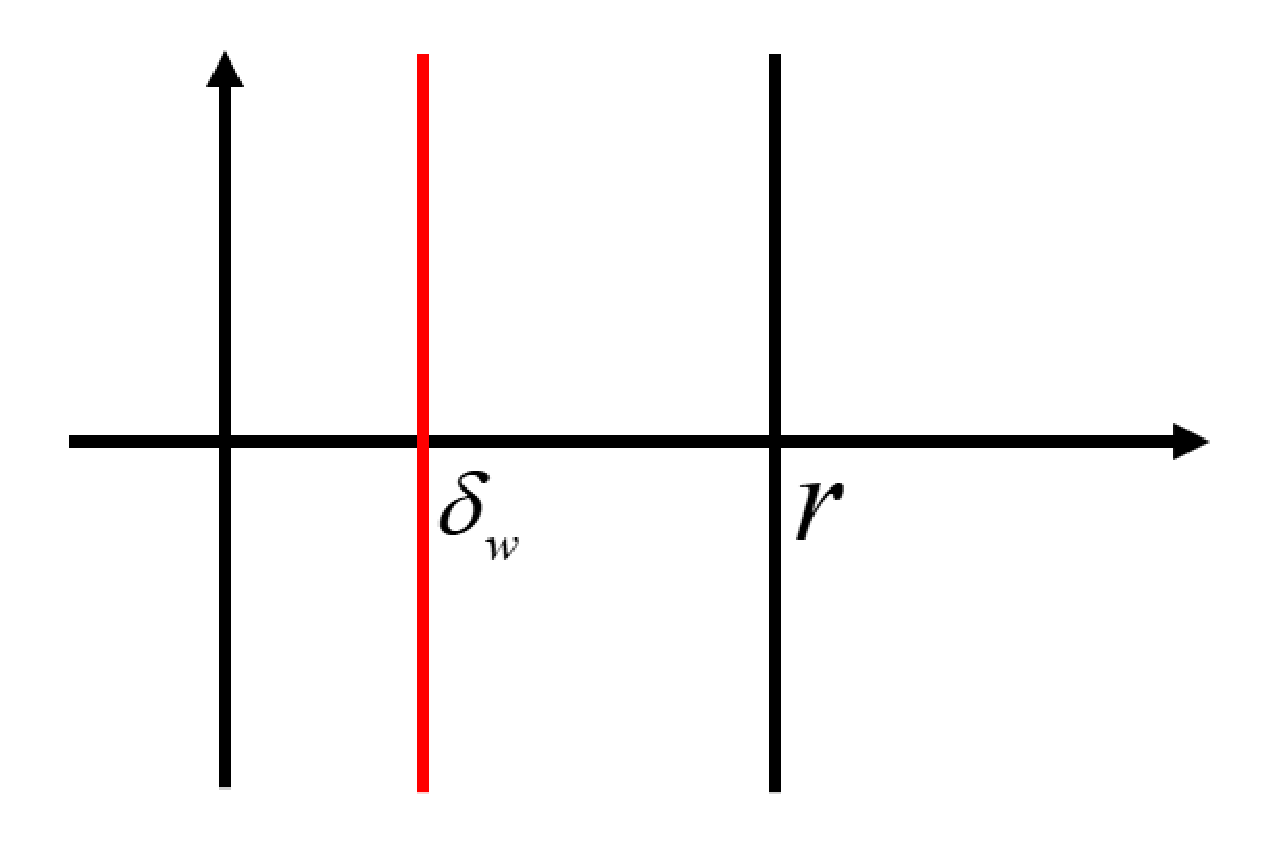
\includegraphics[width=8cm]{14.eps}
        \caption*{}
    \end{figure}
    解得:$\displaystyle\psi(x, y)=\frac{r}{\beta}\left[1-\frac{2}{\sqrt{3}} e^{-\frac{1}{2} k x} \cos \left(\frac{\sqrt{3}}{2} k x-\frac{\pi}{6}\right)\right] \frac{\partial \tau_{x \zeta}}{\partial y} $\\
    \paragraph{东边界区}~{}
    $$\psi(x, y)=\frac{r}{\beta}\left[1-\frac{x}{r}+\frac{1}{k r}\left(e^{-k(r-x)}-1\right)\right] \frac{\partial \tau_{x \zeta}}{\partial y} $$\\
    综合内区、西边界区和东边界区的解可得统一的解的形式:
    \[
        \color{red}
        \boxed{
            \psi=\frac{r}{\beta} f(x) \frac{\partial x_{x \zeta}}{\partial y}
        }
    \]
    \paragraph{讨论}~{}
    \paragraph{环流空间分布特征}~{\centering 图片来自$Introduction \;to \; Physical \;Oceanography$(Robert H. Stewart,2008 pp191)}
    \begin{figure}[H]
        \centering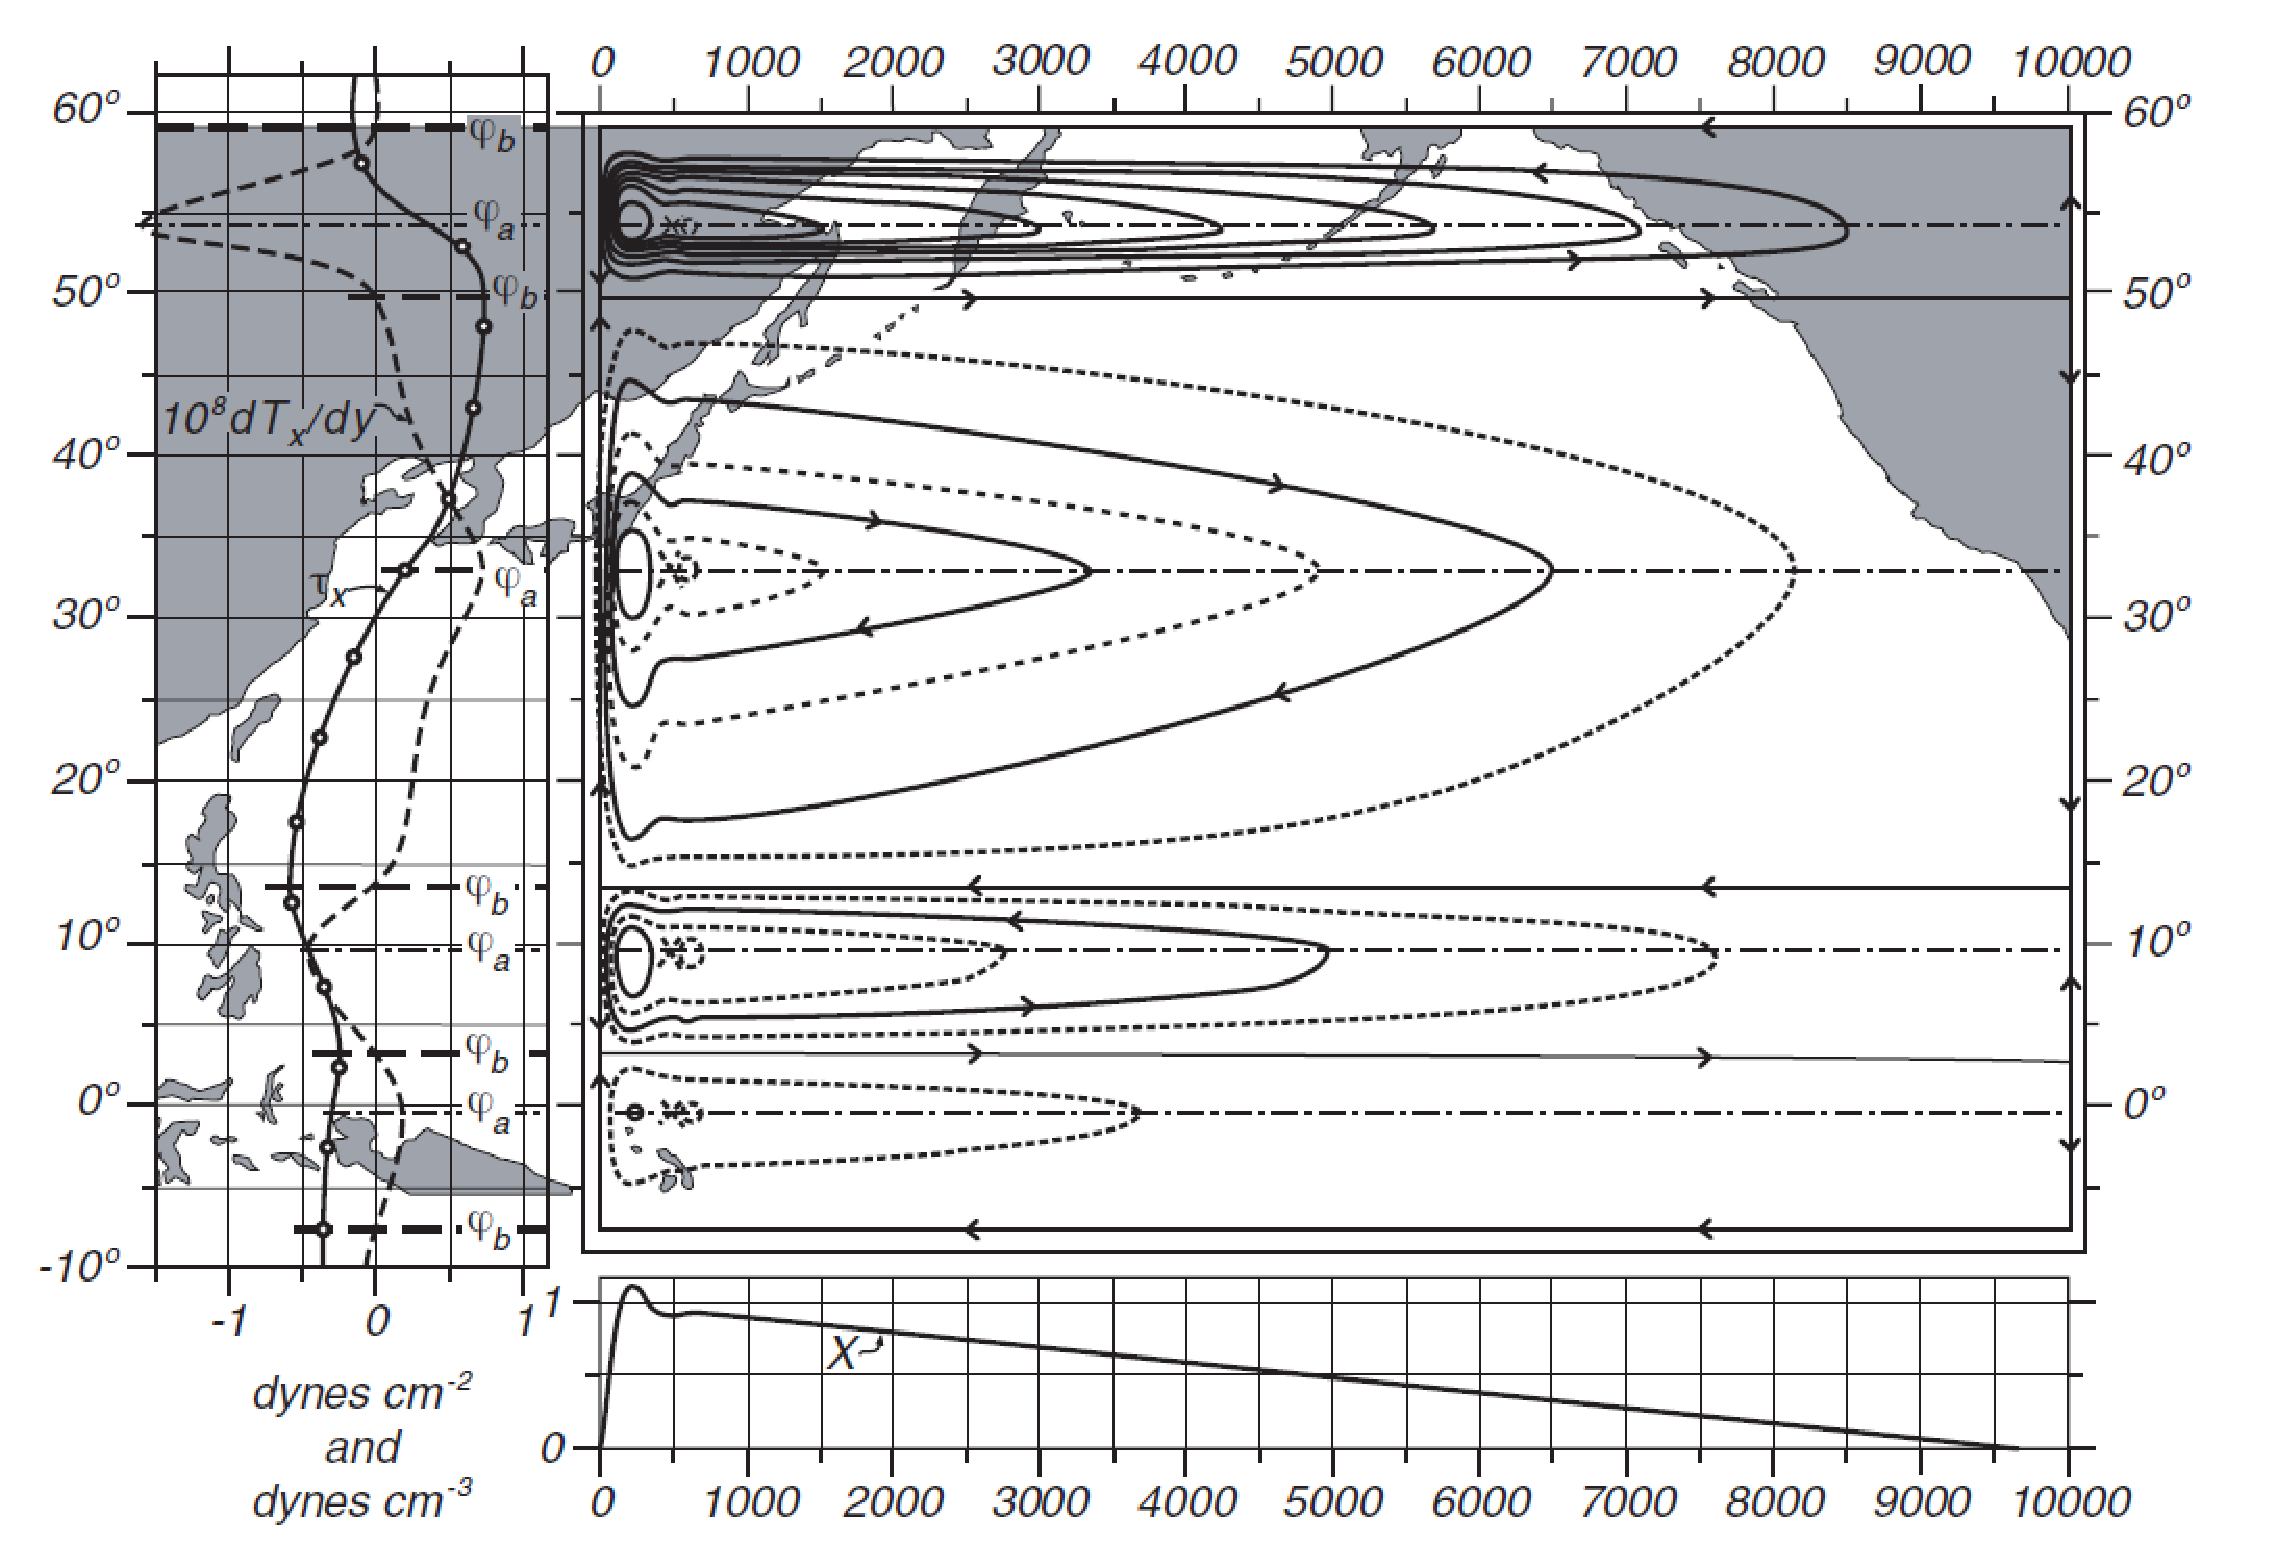
\includegraphics[width=13cm]{15.eps}
        \caption*{}
    \end{figure}
    (1) Gyres之间的分界处位于:$\displaystyle M_y=\frac{\partial \psi}{\partial x}=0$,只有东西向的流动:$\displaystyle f^{\prime}(x)=0/\frac{\partial \tau_{x\zeta}}{\partial y}=0$;\\
    (2) Gyres主轴位于:$\displaystyle M_x=\frac{\partial \psi}{\partial x}=0$只有南北向的流动:$\displaystyle f(x)=0/\frac{\partial^2 \tau_{x\zeta}}{\partial y^2}=0$;\\
    (3) 流动西强东弱.
    \paragraph{大洋西边界区的物质输运特点}~{}
    \[
        \psi_{W}=\frac{r}{\beta} f_{m}(x) \frac{\partial \tau_{x \zeta}}{\partial y}
    \]
    质量输运:
    \[
        \left\{
            \begin{aligned}
                &M_{xW}=-\frac{\partial \psi}{\partial y}=-\frac{r}{\beta} f_{W}(x) \frac{\partial^{2} \tau_{x \zeta}}{\partial y^{2}}\\
                &M_{yW}=\frac{\partial \psi}{\partial x}=\frac{r}{\beta} f_{W}^{\prime}(x) \frac{\partial \tau_{x \zeta}}{\partial y}
            \end{aligned}
        \right.
    \]
    其中,$\displaystyle\left\{\begin{aligned}&f_{W}(x)=1-\frac{2}{\sqrt{3}} e^{-\frac{1}{2} k x} \cos \left(\frac{\sqrt{3}}{2} k x-\frac{\pi}{6}\right)\\&f_{W}^{\prime}(x)=\frac{2}{\sqrt{3}} k e^{-\frac{1}{2} k x} \sin \frac{\sqrt{3}}{2} k x\end{aligned}\right.$
    \begin{figure}[H]
        \centering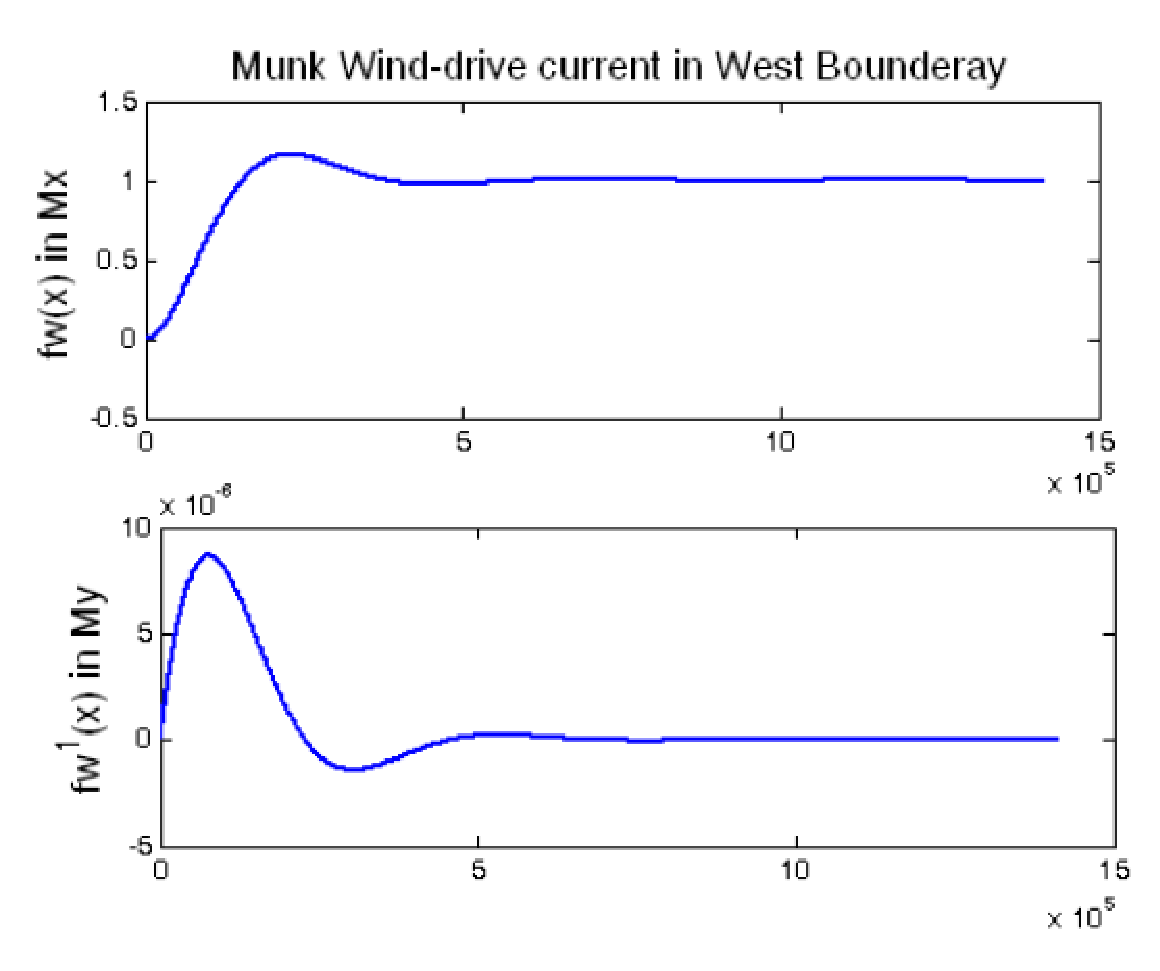
\includegraphics[width=13cm]{16.eps}
        \caption*{\large 随$x$增大而衰减的阻尼振动}
    \end{figure}
    对于任意纬度:
    \[
        M_{y W}=\frac{\partial \psi}{\partial x}=\frac{r}{\beta} f_{w}^{\prime}(x) \frac{\partial \tau_{x \zeta}}{\partial y}
    \]
    因此,$\displaystyle f_W^{\prime}(x)$的极值决定了$\displaystyle M_{yW}$的极值:
    \[
        \begin{aligned}
            &f_W^{\prime\prime}(x)=0 \\
            (\mbox{令}\lambda_W=\frac{2\pi}{\mbox{波数}}=\frac{4\pi}{\sqrt{3}k})
            \Rightarrow &x_{a, b}=\frac{2 \pi}{3 \sqrt{3} k}\left(\frac{1}{6} \lambda_{W}\right), \quad \frac{8 \pi}{3 \sqrt{3} k}\left(\frac{4}{6} \lambda_{W}\right)\\
            \Rightarrow &
            \left\{\begin{aligned}
                &f_{W}^{\prime}\left(x_{a}\right)=k e^{-\pi / 3 \sqrt{3}}\\
                &f_{W}^{\prime}\left(x_{b}\right)=-k e^{-4\pi / 3 \sqrt{3}}
            \end{aligned}\right.
        \end{aligned}
    \]
    \[
        \frac{f_{W}^{\prime}\left(x_{b}\right)} { f_{W}^{\prime}\left(x_{a}\right)}=-e^{-\pi / 3}=-0.17
    \]
    在西边界内,以$x=x_a$(1/6)波长为主轴处有一主流为北向的流动;以$x=x_b$(4/6)波长为主轴处存在一逆流,逆流的量值为主流的0.17倍.\\
    对于任意给定纬度,$\displaystyle f_W(x)$的极值决定$\displaystyle M_{xW}$的极值:
    \[
        f_W^{\prime}(x)=0\Rightarrow x_{1,2}=\frac{2\pi}{\sqrt{3}k},\frac{4\pi}{\sqrt{3}k}\Rightarrow \left\{\begin{aligned}
            &f_{W}\left(x_{1}\right)=1-e^{-\pi/\sqrt{3}}\\
            &f_{W}\left(x_{2}\right)=1+e^{-2\pi/\sqrt{3}}
        \end{aligned}\right.
    \]
    极值在1附近变动.
    \paragraph{缺陷}~{}\\
    (1) 若取$\displaystyle A_l=5\times 10^3 m^2s^{-1}$,西部阻尼振荡的波长比实际大约3倍:$\displaystyle \lambda=\frac{4\pi}{\sqrt{3}k}=\frac{4\pi}{\sqrt{3}}\frac{1}{\sqrt[3]{\beta/A_l}}\approx 200km$;符合实际主流和逆流宽度时,$A_l=10^2m^2s^{-1}$\\
    (2) 西部总流量比实测值小一半.
    \section{海浪}
    \subsection{线性波动理论}
    理论框架:
    \begin{figure}[H]
        \centering 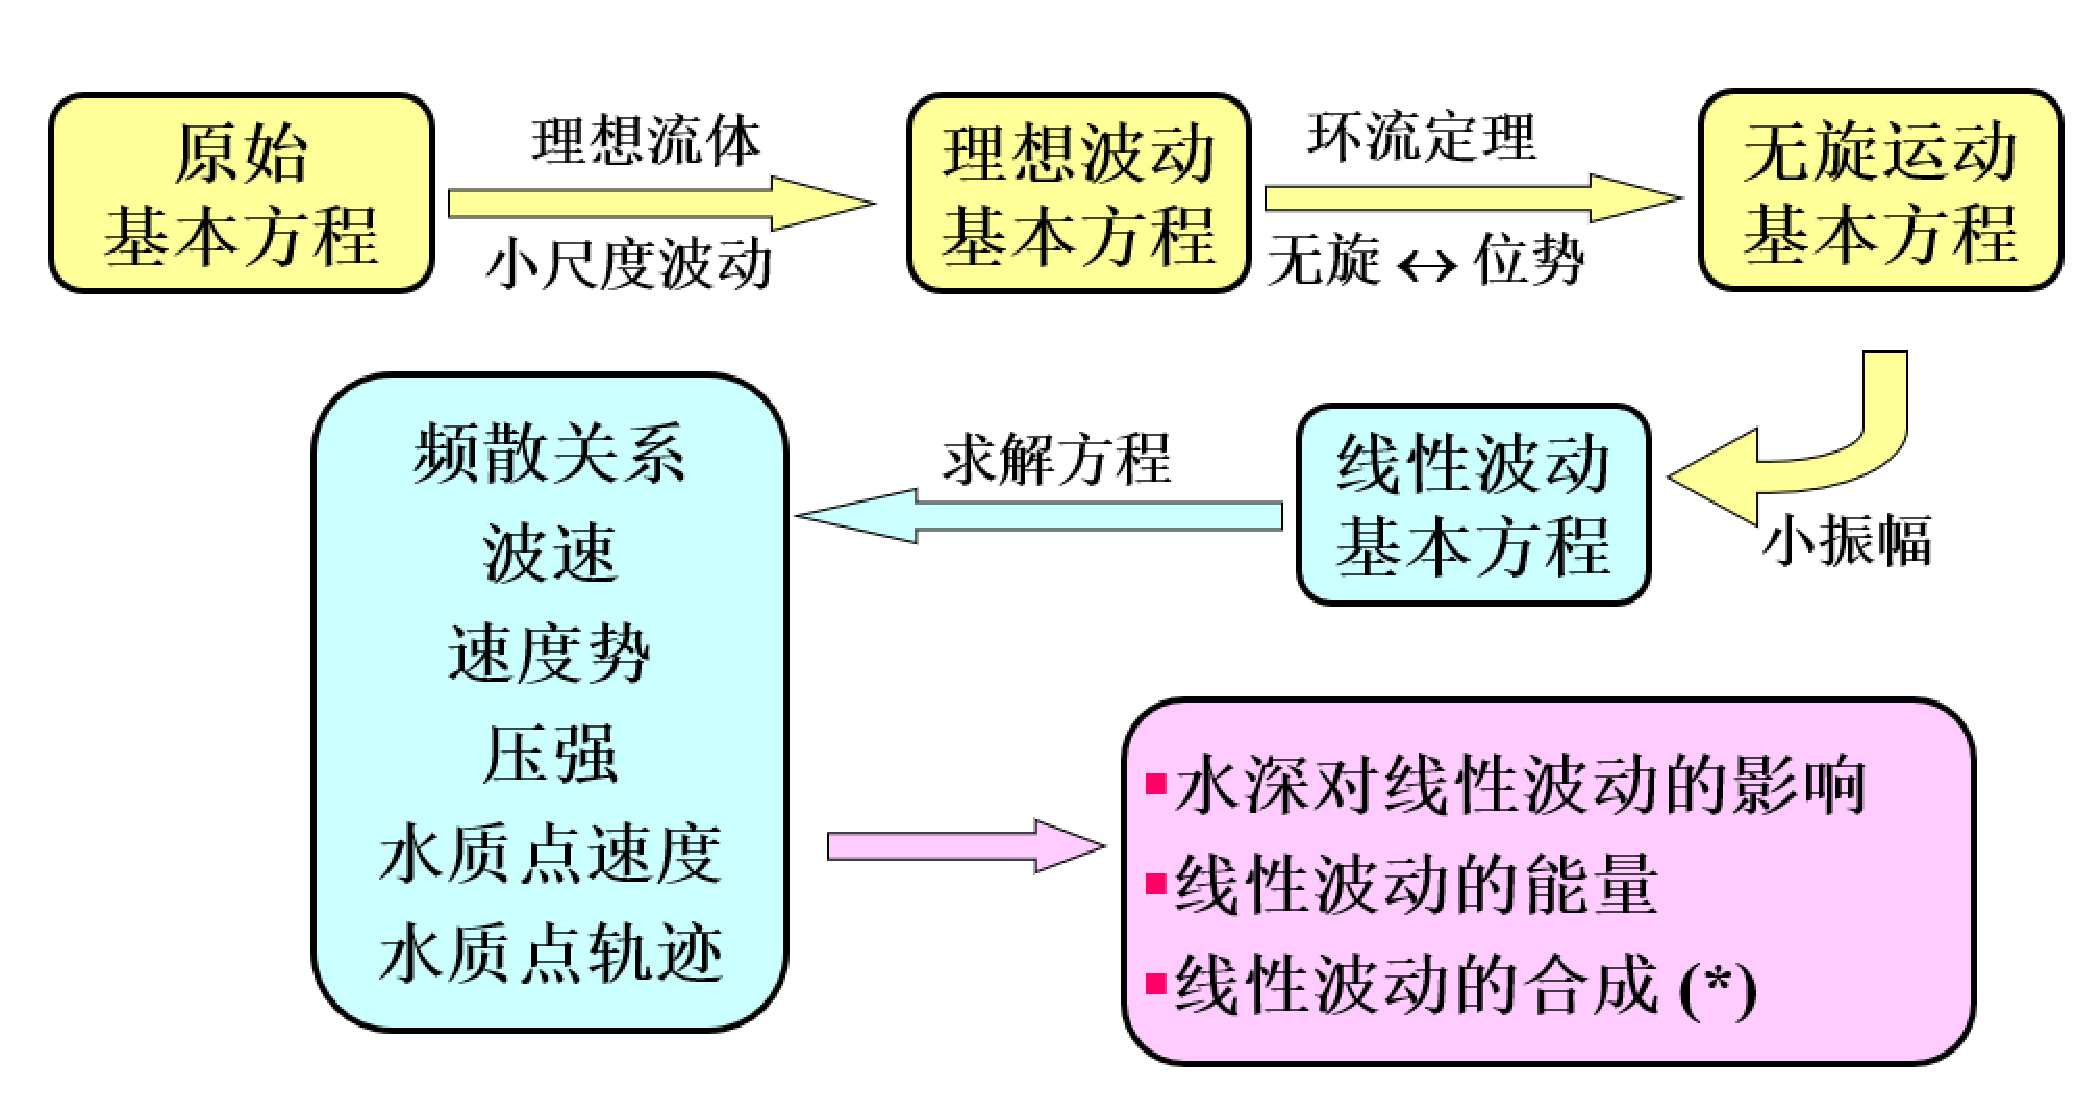
\includegraphics[width=11cm]{17.eps}
        \caption*{}
    \end{figure}
    \subsubsection{无旋运动的基本方程}
    \paragraph{假定及方程}~{}\\
    (1) 海水均匀不可压缩;\\
    (2) 理想流体;\\
    (3) 短周期小尺度波动;\\
    (4) 重力为唯一的外力;\\
    (5) 忽略分子粘性项、科氏力、引潮力和湍摩擦力.\\
    控制方程:
    \[
        \left\{
            \begin{aligned}
                &\frac{d\vec{V}}{dt}=\frac{\partial \vec{V}}{\partial t}+(\vec{V}\cdot\nabla)\vec{V}=-\frac{1}{\rho}\nabla p-\vec{g}\\
                &\frac{\partial u}{\partial x}+\frac{\partial v}{\partial y}+\frac{\partial w}{\partial z}
            \end{aligned}
        \right.
    \]
    边界条件:
    \[
        \left\{
            \begin{aligned}
                &z=\zeta(\mbox{海面}):{{\partial \zeta } \over {\partial t}} + u{{\partial \zeta } \over {\partial x}} + v{{\partial \zeta } \over {\partial y}} = w,p_I=p_a(x,y,t)\\
                &\mbox{固体边界处}:V_n=0
            \end{aligned}
        \right.
    \]
    \paragraph{环流定理}~{}
    \begin{figure}[H]
        \centering 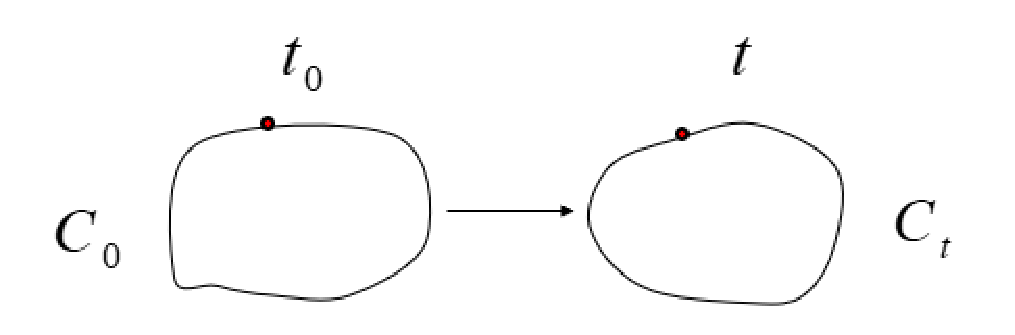
\includegraphics[width=7cm]{18.eps}
        \caption*{}
    \end{figure}
    $C_t$上的环流:$\displaystyle \Gamma(t)=\oint\limits_{ct}udx+vdy+wdz$
    \[
    \begin{aligned}
        &\Rightarrow \frac{d \Gamma(t)}{d t}=\oint\limits_{c t} \left(\frac{d u}{d t} d x+\frac{d v}{d t} d y+\frac{d w}{d t} d z\right)+\underbrace{\oint\limits_{c t} \left(u d u+v d v+w d w\right)}_{=\frac{1}{2} \oint\limits_{c t} d u^{2}+d v^{2}+d w^{2}=0}\\
        &\Rightarrow \frac{d \Gamma(t)}{d t}=\oint\limits_{c t} \frac{d \vec{V}}{d t} \cdot d \vec{l}
    \end{aligned}
    \]
    环流的实质微商等于加速度的环流.
    \[
        \frac{d \Gamma(t)}{d t}=\oint\limits_{c t}\left(-\frac{1}{\rho} \frac{\partial p}{\partial x}\right) d x+\left(-\frac{1}{\rho} \frac{\partial p}{\partial y}\right) d y+\left(-\frac{1}{\rho} \frac{\partial p}{\partial z}-g\right)d z=\oint\limits_{c t} d\underbrace{\left(-\frac{p}{\rho}-g z\right)}_{\mbox{单值函数}}=0 
    \]
    $\color{red}\mbox{环流定理}$:对不可压缩的理想流体,由相同质点构成的封闭曲线上的环流不随时间而变。
    \paragraph{无旋运动的基本方程和边界条件}~{}\\
    若在重力场中,理想流体于起始时刻为静止或匀速运动,则任何时刻,对任何封闭曲线有:$\Gamma(t)=0$,根据Stokes定理:
    \[
        \Gamma(t)=\oint\limits_{c t} \vec{V} \cdot d \vec{l}=\iint\limits_{s} \nabla \times \vec{V} d \sigma=0\Rightarrow\nabla\times\vec{V}=\Rightarrow\vec{V}=\nabla \varphi
    \]
    运动方程:
    \[
            \frac{d\vec{V}}{dt}=\frac{\partial \vec{V}}{\partial t}+(\vec{V}\cdot\nabla)\vec{V}=-\frac{1}{\rho}\nabla p-\vec{g}
    \]
    \[
        \begin{aligned}
            &\Rightarrow \frac{d\vec{V}}{dt}=\frac{\partial \vec{V}}{\partial t}+\frac{1}{2}\nabla(\vec{V}\cdot\vec{V})=-\nabla\frac{p-p_0}{\rho}-\nabla(gz)\\
            &\Rightarrow \nabla\frac{\partial \varphi}{\partial t}+\frac{1}{2}\nabla(\nabla\varphi\cdot\nabla\varphi)=-\nabla\frac{p-p_0}{\rho}-\nabla(gz)\\
            &\Rightarrow \frac{\partial \varphi}{\partial t}+\frac{1}{2}(\nabla \varphi)(\nabla \varphi)+\frac{p-p_{0}}{\rho}+g z=0
        \end{aligned}
    \]
    连续方程:
    \[
        \Delta \varphi=\frac{\partial^{2} \varphi}{\partial x^{2}}+\frac{\partial^{2} \varphi}{\partial y^{2}}+\frac{\partial^{2} \varphi}{\partial z^{2}}=0
    \]
    运动学边界条件: 
    \[
        \begin{aligned}
            \mbox{海面}:&\left.\left(\frac{\partial \zeta}{\partial t}+\frac{\partial \varphi}{\partial x} \frac{\partial \zeta}{\partial x}+\frac{\partial \varphi}{\partial y} \frac{\partial \zeta}{\partial y}\right)\right|_{z=\zeta}=\left.\frac{\partial \varphi}{\partial z}\right|_{z=\zeta} \\
            \mbox{固定边界}:&\frac{\partial \varphi}{\partial n}=0
        \end{aligned}
    \]
    动力学边界条件: 
    \[
        \begin{aligned}
            &p_{I}=p_{a}(x, y, t) \\
            &{\left.\left[\frac{\partial \varphi}{\partial t}+\frac{1}{2}(\nabla \varphi)(\nabla \varphi)\right]\right|_{z=\zeta}+g \zeta=0}
        \end{aligned}
    \]
    \subsubsection{线性波动}
    \paragraph{假定}~{}\\
    (1) 均质不可压理想流体;\\
    (2) 波动的振幅相对波长很小;\\
    (3) 设水域广阔等深;\\
    (4) 波动只沿x方向传播.\\
    小振幅假定$\displaystyle:\Rightarrow\left\{\begin{aligned}&\varphi\mbox{的微商乘积项可忽略}\\&\left.\left.\frac{\partial \varphi}{\partial z}\right|_{z=\zeta} \approx \frac{\partial \varphi}{\partial z}\right|_{z=0},\left.\left.\frac{\partial \varphi}{\partial t}\right|_{z=\zeta} \approx \frac{\partial \varphi}{\partial t}\right|_{z=0}\end{aligned}\right.$
    \paragraph{方程简化}~{}\\
    \begin{spacing}{2}
        运动方程:$\displaystyle \frac{\partial \varphi}{\partial t}+\cancel{\frac{1}{2}(\nabla \varphi)(\nabla \varphi)}+\frac{p-p_{0}}{\rho}+g z=0$\\
    连续方程:$\displaystyle\Delta \varphi=\frac{\partial^{2} \varphi}{\partial x^{2}}+\cancel{\frac{\partial^{2} \varphi}{\partial y^{2}}}+\frac{\partial^{2} \varphi}{\partial z^{2}}=0$\\
    边界条件:$\displaystyle \left\{\begin{aligned}
        &\left.\left(\frac{\partial \zeta}{\partial t}+\cancel{\frac{\partial \varphi}{\partial x} \frac{\partial \zeta}{\partial x}+\frac{\partial \varphi}{\partial y} \frac{\partial \zeta}{\partial y}}\right)\right|_{z=\zeta}=\left.\frac{\partial \varphi}{\partial z}\right|_{z=\zeta} \\
        &\frac{\partial \varphi}{\partial n}=\left.0 \Rightarrow \frac{\partial \varphi}{\partial z}\right|_{z=-d}=0 \\
        &{\left.\left[\frac{\partial \varphi}{\partial t}+\cancel{\frac{1}{2}(\nabla \varphi)(\nabla{\varphi})}\right]\right|_{z=\zeta}+g \zeta=0}
        \end{aligned}\right.$
    \end{spacing}
    因此,$\color{red}\mbox{线性波动的基本方程}$:
    \begin{numcases}{}
        \frac{\partial \varphi}{\partial t}+\frac{p-p_{0}}{\rho}+g z=0 \label{lw1}\\
        \frac{\partial^{2} \varphi}{\partial x^{2}}+\frac{\partial^{2} \varphi}{\partial z^{2}}=0 \label{lw2}\\
        \left.\frac{\partial \varphi}{\partial z}\right|_{==0}=\frac{\partial \zeta}{\partial t}\label{lw4} \\
        \left.\frac{\partial \varphi}{\partial z}\right|_{z=-d}=0 \label{lw4}\\
        \left.\frac{\partial \varphi}{\partial t}\right|_{z=0}+g \zeta=0\label{lw5}
    \end{numcases}
    $(\ref{lw5})$代入$(\ref{lw3})$中:
    \[
        \left.\left(\frac{\partial \varphi}{\partial z}+\frac{1}{g} \frac{\partial^{2} \varphi}{\partial t^{2}}\right)\right|_{z=0}=0\label{lw6}
    \]
    \paragraph{求解}~{}\\
    对前进波:
    \begin{equation}
        \varphi=\varphi_0(z)\cos(kx-\omega t) \label{*}
    \end{equation}
    $(\ref{*})$代入$(\ref{lw2})$中:
    \begin{equation}
        \varphi_0(z)=Ae^{kz}+Be^{-kz} \label{lw7}
    \end{equation}
    $(\ref{*})$代入$(\ref{lw6})$中(海面):
    \begin{equation}
        \left.\left[\frac{\partial \varphi_{0}(z)}{\partial z}-\frac{\omega^{2}}{g} \varphi_{0}(z)\right]\right|_{z=0}=0 \label{lw8}
    \end{equation}
    $(\ref{*})$代入$(\ref{lw4})$中(海底):
    \begin{equation}
        \left.\frac{d \varphi_{0}(z)}{d z}\right|_{z=-d}=0\label{lw9}
    \end{equation}
    $(\ref{lw7})$代入$(\ref{lw8})$中:
    \begin{equation}
            \left(\omega^{2}-g k\right) A+\left(\omega^{2}+g k\right) B =0 \label{lw10}
    \end{equation}
    $(\ref{lw7})$代入$(\ref{lw9})$中:
    \begin{equation}
        e^{-k d} A-e^{k d} B =0 \label{lw11}
    \end{equation}
    联立$(\ref{lw10}),(\ref{lw11})$,有非零解的条件为:
    \[
        \left|\begin{array}{cc}
            e^{-k d} & -e^{k d} \\
            \left(\omega^{2}-g k\right) & \left(\omega^{2}+g k\right)
            \end{array}\right|=0\Rightarrow \color{red}\mathop{\omega^2=gk\operatorname{th} kd}\limits_{\color{red}\mbox{频散关系}}
    \]
    频散关系表示波动频率和波数之间的关系,代表某种波动的性质.\\
    波速:$\displaystyle c=\frac{\lambda}{T}=\frac{2 \pi / k}{2 \pi / \omega}=\frac{\omega}{k} \Rightarrow c^{2}=\frac{\omega^{2}}{k^{2}}=\frac{g}{k} \text { th } k d $\\
    波速与水深和波动性质有关系.\\
    由$(\ref{lw11}):A e^{-k d}=B e^{k d}=\frac{1}{2} D\Rightarrow A=\frac{D}{2} / e^{-k d} ; \quad B=\frac{D}{2} / e^{k d}$\\
    代入$(\ref{*})$:
    \begin{equation}
        \varphi=D\operatorname{ch}[k(z+d)]\cos (kx-\omega t) \label{lw12}
    \end{equation}
    $(\ref{lw12})$代入$(\ref{lw5})$中:
    \[
        \zeta=-\frac{\omega}{g} D \operatorname{ch} k d  \sin (k x-\omega t)=a\sin (kx-\omega t)
    \]
    速度势的解:
    \begin{equation}
        \varphi=-\frac{a g}{\omega} \frac{\operatorname{ch}[k(z+d)]}{\operatorname{ch} k d} \cos (k x-\omega t) \label{lw13}
    \end{equation}
    $(\ref{lw13})$代入$(\ref{lw1})$中,可得压强分布:
    \[
        p=p_{0}+\rho g a \frac{\operatorname{ch}[k(z+d)]}{\operatorname{ch} k d} \sin (k x-\omega t)-\rho g z
    \]
    水质点速度:
    \[
        \begin{aligned}
            &u=\frac{\partial \varphi}{\partial x}=\frac{a g k}{\omega} \frac{\operatorname{ch}[k(z+d)]}{\operatorname{ch} k d} \sin (k x-\omega t) \\
            &w=\frac{\partial \varphi}{\partial z}=-\frac{{agk}}{\omega} \frac{\operatorname{sh}[k(z+d)]}{\operatorname{ch} k d} \cos (k x-\omega t)
            \end{aligned}
    \]
    水质点运动轨迹($x_0,z_0$)为平衡位置:
    \[
        \frac{\left(x-x_{0}\right)^{2}}{\left[a \frac{\operatorname{ch}\left[k\left(d+z_{0}\right)\right]}{\operatorname{sh} k d}\right]^{2}}+\frac{\left(z-z_{0}\right)^{2}}{\left[a \frac{\operatorname{sh}\left[k\left(d+z_{0}\right)\right]}{\operatorname{sh} k d}\right]^{2}}=1
    \]
    \paragraph{解的讨论}~{}
    \begin{figure}[H]
        \centering 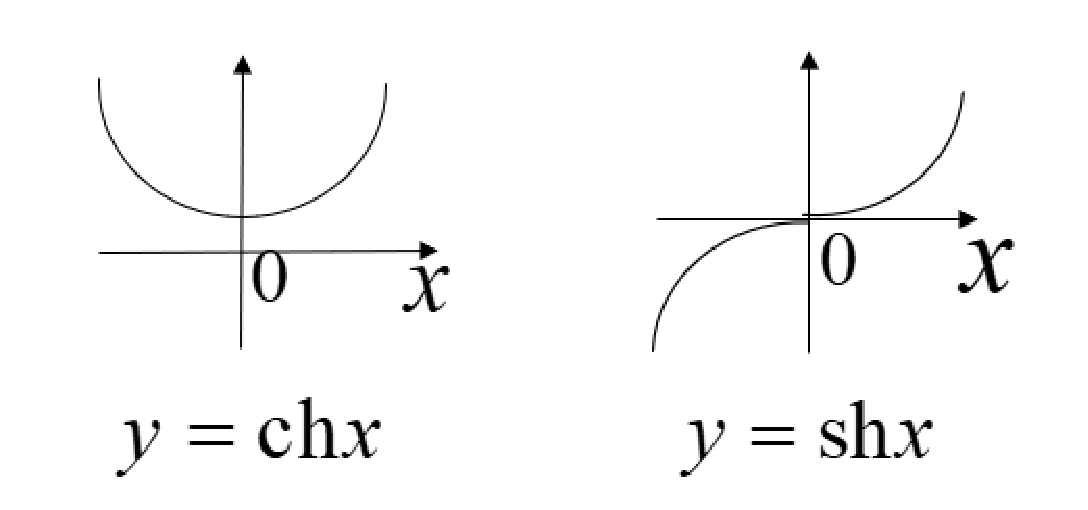
\includegraphics[width=8cm]{19.eps}
        \caption*{}
    \end{figure}
    (1) 线性波动水质点轨迹为椭圆,长轴为$x$方向;\\
    (2) 椭圆长轴和短轴均与$z_0$ 有关,与 $x_0$ 无关;\\  
    (3) 长轴和短轴均随平衡位置的加深而减小;\\
    (4) 在海底水质点做水平运动.
    \subsubsection{水深对线性波动的影响}
    \paragraph{深水波($d>\frac{1}{2}\lambda$)}~{}\\
    \begin{spacing}{2}
        $\displaystyle kd=\frac{2\pi}{\lambda}d\rightarrow \infty$
    $\displaystyle \operatorname{sh}kd=\operatorname{ch}\approx \frac{1}{2} e^{kd},\operatorname{th}kd\approx 1$\\
    频散关系:$\displaystyle \omega^{2}=g k \text { th } k d \Rightarrow \omega^{2}=g k$\\
    波速:$\displaystyle c^{2}=\frac{g}{k} \operatorname{th} k d \Rightarrow c^{2}=\frac{g}{k}$\\
    深水波的角频率和波速与水深无关,只与波动性质(波数或波长)有关.\\
    \end{spacing}
    速度势:
    \[
    \begin{aligned}
        \varphi&=-\frac{a g}{\omega} \frac{\operatorname{ch}[k(z+d)]}{\operatorname{ch} k d} \cos (k x-\omega t)\\
        \left(\operatorname{ch}[k(z+d)]\approx\frac{1}{2}e^{kd}(\operatorname{ch}kz+\operatorname{sh}kz)\right)\quad&=-\frac{a g}{\omega} e^{kz} \cos (k x-\omega t)
    \end{aligned}
    \]
    压强分布:$\displaystyle p=p_{0}+\rho g a \frac{\operatorname{ch}[k(z+d)]}{\operatorname{ch} k d} \sin (k x-\omega t)-\rho g z$\\
    水质点速度:$\displaystyle u=a\omega e^{kz}\sin(kx-\omega t),w=-a\omega e^{kz}\cos (kx-\omega t)$\\
    水质点轨迹:$\displaystyle \left(x-x_{0}\right)^{2}+\left(z-z_{0}\right)^{2}=\left(a e^{k_{0}}\right)^{2}$\\
    深水波水质点运动轨迹为圆,半径随水质点平衡位置的深度增加而减小,当达到很大深度时,半径无限小,运动消失——表面波性质.
    \paragraph{浅水波($d<\frac{1}{20}\lambda$)}~{}
    $\displaystyle kd=\frac{2\pi}{\lambda}d\rightarrow 0$\\
    幂级数展开:$\displaystyle \begin{aligned} &\operatorname{sh} x=x+\frac{x^{3}}{3 !}+\cdots+\frac{x^{2 n+1}}{(2 n+1) !}+\cdots(-\infty<x<\infty) \\
    &\operatorname{ch} x=1+\frac{x^{2}}{2 !}+\cdots+\frac{x^{2 n}}{(2 n) !}+\cdots\end{aligned}$\\
    $\displaystyle \operatorname{sh}kd\approx kd,\operatorname{ch}kd\approx 1+\frac{k^2 d^2}{2}\approx 1,\operatorname{th}\approx kd$\\
    \begin{spacing}{2}
        频散关系:$\displaystyle \omega^{2}=g k \text { th } k d \Rightarrow \omega^{2}=gd k^2$\\
    波速:$\displaystyle c^{2}=\frac{g}{k} \operatorname{th} k d \Rightarrow c^{2}=gd$\\
    波速只与水深有关,而与波动性质无关.\\
    速度势:$\displaystyle \varphi=-\frac{a g}{\omega}\left[1+\frac{k^{2}(d+z)^{2}}{2}\right] \cos (k x-\omega t)$\\
    压强分布:$p=p_0+\rho g(\zeta-z)$\\
    压强分布近似为静压分布.\\
    水质点速度:$\displaystyle u=\frac{a \omega}{k d} \sin (k x-\omega t) ,   w=-a \omega\left(1+\frac{z}{d}\right) \cos (k x-\omega t)$\\
    质点水平速度显著大于铅直速度.\\
    水质点轨迹:$\displaystyle \frac{\left(x-x_{0}\right)^{2}}{\left(\frac{a}{k d}\right)^{2}}+\frac{\left(z-z_{0}\right)^{2}}{\left[a\left(1+\frac{z_{0}}{d}\right)\right]^{2}}=1$\\
    浅水波水质点运动轨迹为椭圆,水平轴(长轴)不随深度改变,短轴随深度增加逐渐减小.
    \end{spacing}
    \begin{figure}[H]
        \centering 
        \subfigure{
        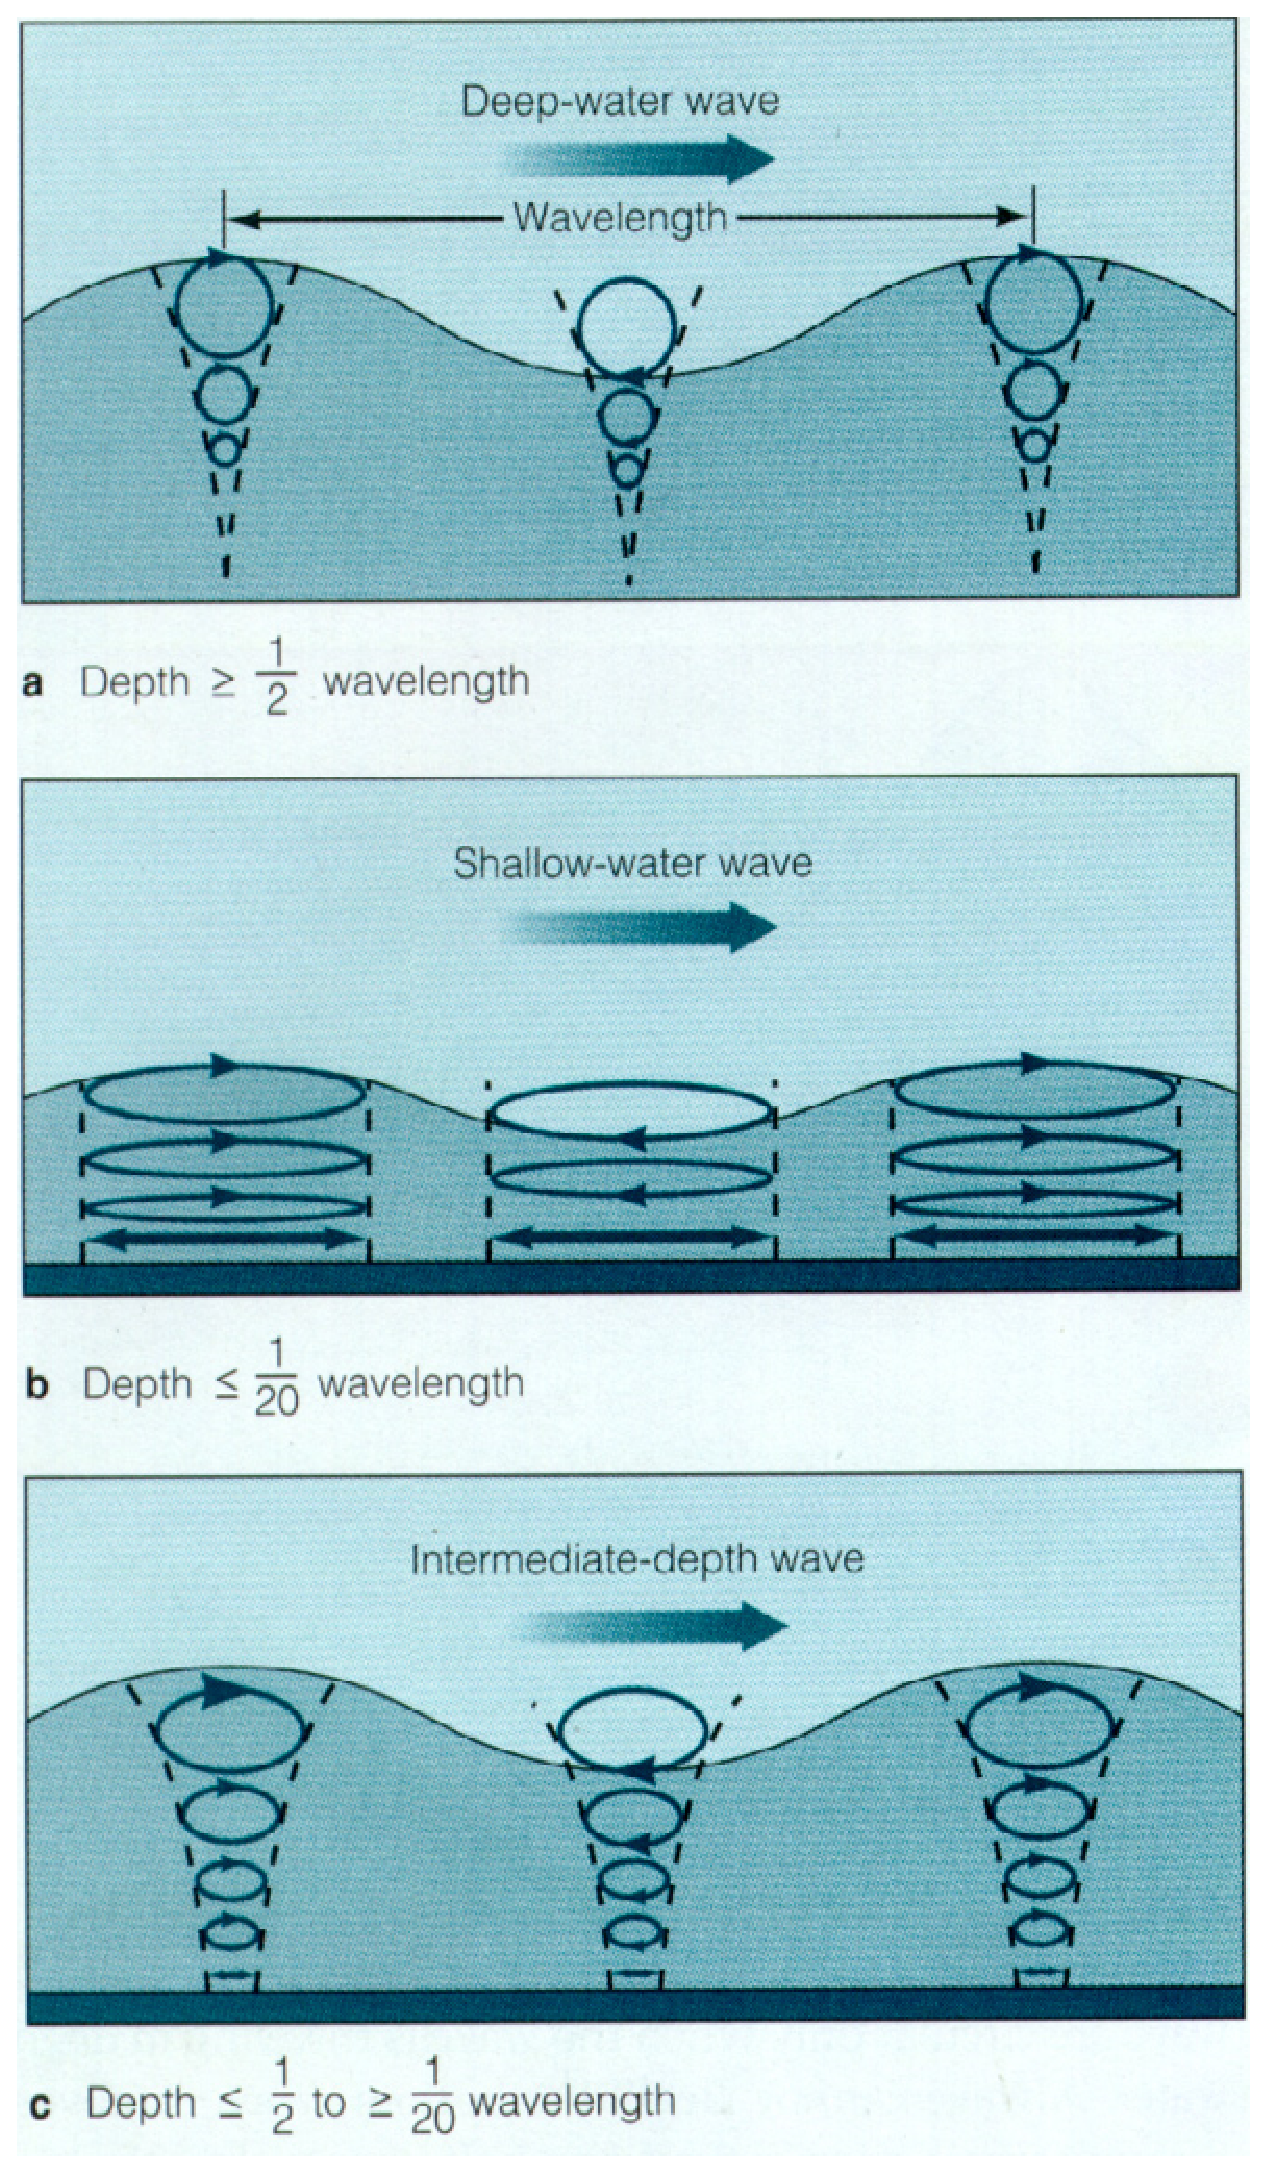
\includegraphics[width=8cm]{20.eps}
        }
        \subfigure{
        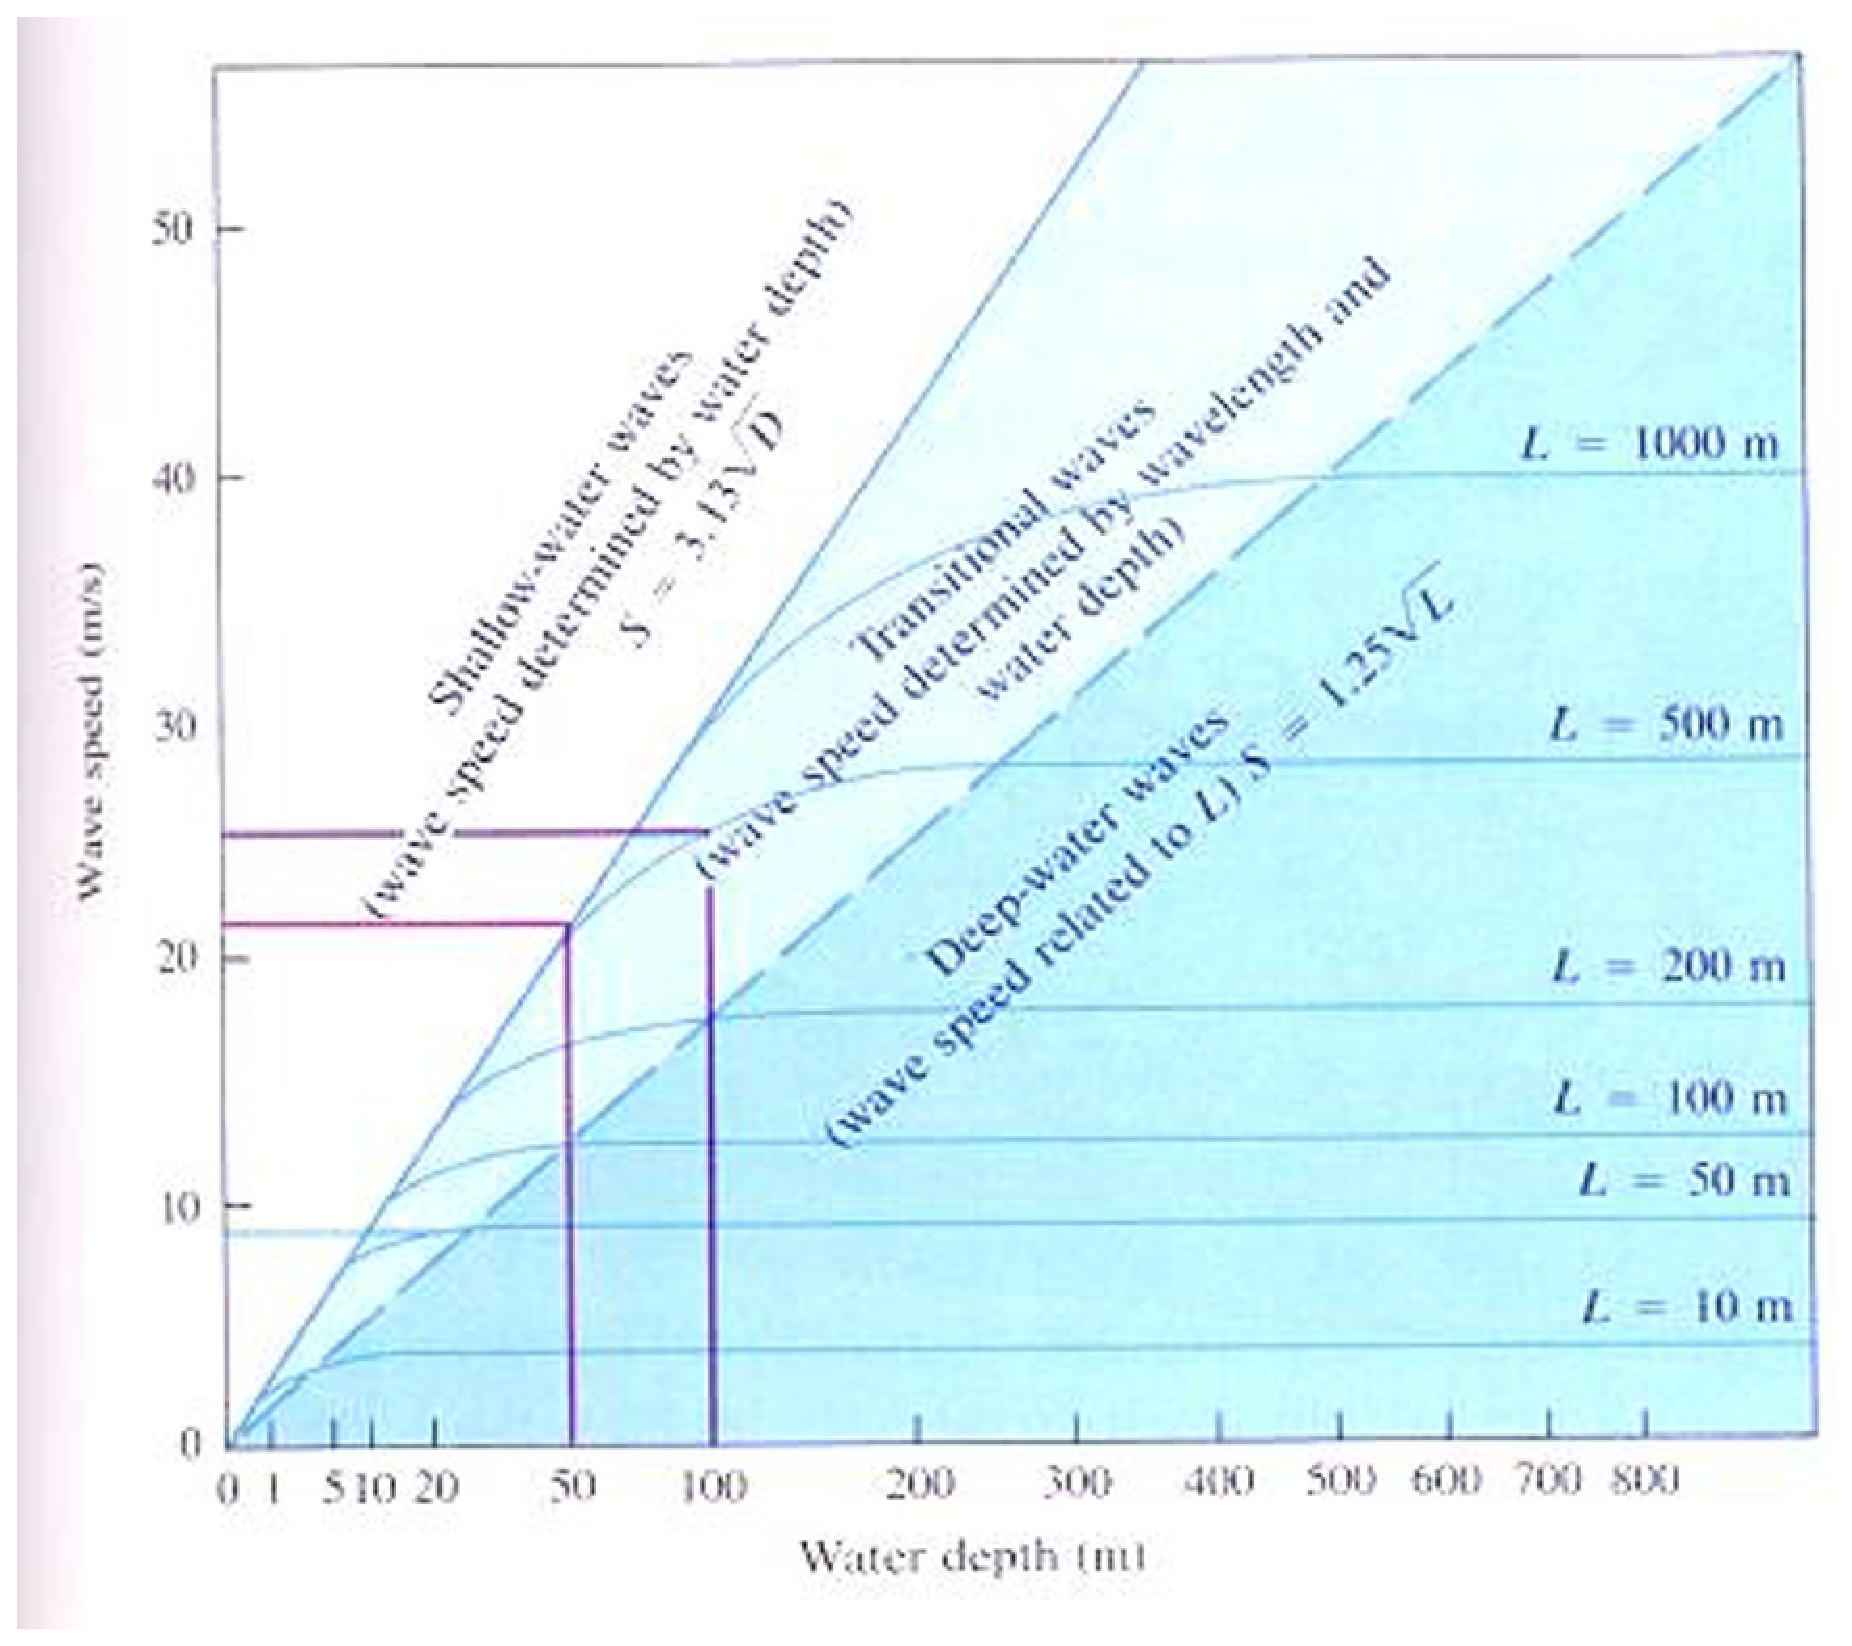
\includegraphics[width=10cm]{21.eps}
        }
        \caption*{}
    \end{figure}
    \subsubsection{线性波动的能量}\label{energy}
    以下都是讨论一个波长范围内的线性波动能量,示意图如下:
	\begin{figure}[H]
		\centering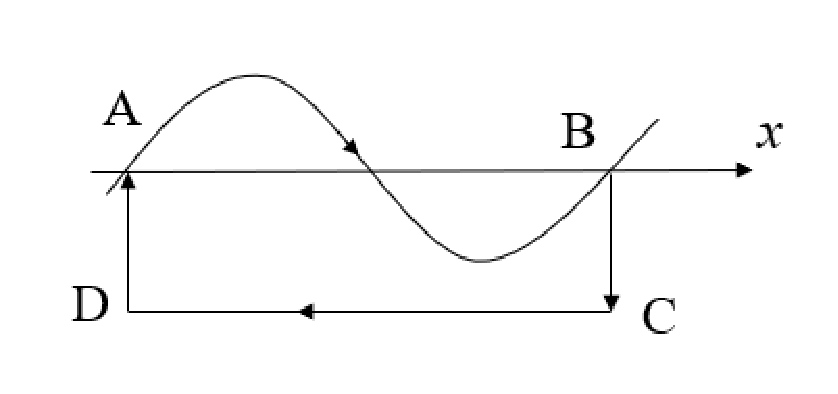
\includegraphics[width=9cm]{22.eps}
		\caption{波动示意图}\label{fig:2} 
	\end{figure}
	\paragraph{动能}~{}\\
	根据动能定义,
	\[
	\begin{aligned}
	    {E_k} &= {1 \over 2}m{V^2}\\
	    &=\int_{0}^{\lambda}\left[\int_{-d}^{\zeta} \frac{1}{2} \rho\left(u^{2}+w^{2}\right) d z\right] d x\\
	    &=\frac{\rho}{2} \int_{0}^{\lambda} \int_{-d}^{\zeta}\left[\left(\frac{\partial \varphi}{\partial x}\right)^{2}+\left(\frac{\partial \varphi}{\partial z}\right)^{2}\right] d z d x\\
	\end{aligned}
	\]
	\indent
	根据格林第一定理:
	$$\iiint_{\tau} \varphi \Delta \varphi d \tau+\iiint_{\tau} \nabla \varphi \cdot \nabla \varphi d \tau=\varoiint_{s} \varphi \frac{\partial \varphi}{\partial{n}	} d s$$
	又因为对于不可压流体$\Delta{\varphi}=0$,因此:
	\[
	\begin{aligned}
		{E_k} &= {1 \over 2}m{V^2}\\
	    &=\frac{\rho}{2} \iiint_{\tau} \nabla \varphi \cdot \nabla \varphi d \tau\\
	    &=\frac{\rho}{2} \varoiint_{s} \varphi \frac{\partial \varphi}{\partial n} d s\\
	    &=\frac{\rho}{2} \oint_{c} \varphi \frac{\partial \varphi}{\partial n} d l
	\end{aligned}
	\]
    其中,$c$为图2中的闭合有向曲线。
    \par
    根据对称性,$\overrightarrow{BC}$与$\overrightarrow{DA}$上的积分值等大反向,根据边界条件,在海底
    ${{\partial \phi } \over {\partial n}} = {{\partial \phi } \over {\partial z}}{|_{z =  - d}} = 0$。因此:
    \[
    {E_k} = {\rho  \over 2}\int_0^\lambda  {\left.(\varphi {{\partial \varphi } \over {\partial z}}) \right|_{z = \zeta}dx}
    \]
    \indent
    再根据小振幅假定,振幅相对波长很小,$\zeta\approx 0$,因此:
    \[
    {E_k} = {\rho  \over 2}\int_0^\lambda  {\left.(\varphi {{\partial \varphi } \over {\partial z}}) \right|_{z = 0}dx} 
    \]
	\indent
	带入线性波动的解:
	\[
	\begin{aligned}
		\varphi  &=  - {{ag} \over \omega }{{{\rm{ch}} [k(d + z)]} \over {{\rm{ch}} kd}}\cos (kx - \omega t)\\
		\Rightarrow\frac{\partial \varphi}{\partial z} & =-\frac{agk\mathrm{sh}\left[k\left(d+z\right) \right]}{\omega \mathrm{ch}\left(kd\right)}\cos\left(kx-\omega t\right)
	\end{aligned}
	\]
	\[
	\begin{aligned}
	{E_k} &= {\rho  \over 2}\int_0^\lambda  {\left. {{ag} \over \omega }{{{\rm{ch}} [k(d + z)]} \over {{\rm{ch}} kd}}\cos (kx - \omega t)\frac{agk\mathrm{sh}\left[k\left(d+z\right) \right]}{\omega \mathrm{ch}\left(kd\right)}\cos\left(kx-\omega t\right) \right|_{z = 0}dx} \\
	&= \frac{\rho}{2\omega^2} a^2g^2k \mathrm{th}kd \int_0^\lambda {\mathrm{cos}^2(kx-\omega t)dx}\\
	&= \frac{\rho}{2\omega^2} a^2g^2 \mathrm{th}kd \int_0^{2\pi} {\mathrm{cos}^2(\theta-\omega t)d\theta}\\
	&= \frac{\rho}{2\omega^2} a^2g^2 \pi\mathrm{th}kd
	\end{aligned}
	\]
	\indent
	再带入频散关系:${\omega ^2} = gk {\rm th} kd$以及$k=\frac{2\pi}{\lambda}$:
	\[
	E_k=\frac{1}{4}\rho ga^2\lambda
	\]
	\paragraph{势能}~{}\\
	根据势能的定义:
	\[
	\begin{aligned}
		E_p &= mgh\\
		    &= \int_0^\lambda  {\int_0^\zeta  {\rho gzdzdx} }\\
		    &= \rho g\int_0^\lambda  {\int_0^\zeta  {{1 \over 2}d{z^2}dx} } \\
		    &= {1 \over 2}\rho g\int_0^\lambda  {\zeta^2 dx } \\
		    &= {1 \over 2}\rho g\int_0^\lambda  {{a^2}{{\sin }^2}(kx - \omega t)dx}\\
		    &= {1 \over 4}\rho g{a^2}\lambda
	\end{aligned}
	\]
	\paragraph{总能量}~{}\\
	一个波长内的总能量为动能和势能之和:
	\[
	E = {E_K} + {E_P} = {1 \over 2}\rho g{a^2}\lambda
	\]
	\indent
	进而可以计算单位表面面积水柱的平均总能量 :
	\[
	\bar E = \frac{E}{\lambda} = {1 \over 2}\rho g{a^2}
	\]
	\paragraph{平均能量通量及水深影响}~{
    }
	能量通量是单位时间内通过垂直于波动传播方向断面的能量,等于单位时间内通过某断面的波动能量等于该断面外侧有效压力所做的功。根据线性波动的势函数方程:
	\[
	{{\partial \varphi } \over {\partial t}} + {{p - {p_0}} \over \rho } + gz = 0
	\]
	\indent
	则有效压强为:
	\[
	{p_e} =  - \rho {{\partial \varphi } \over {\partial t}}
	\]
	\indent
	根据能量通量定义:
	\[
	P = \int_{ - d}^\zeta  {{p_e}udz} = \int_{ - d}^\zeta  { - \rho {{\partial \varphi } \over {\partial t}}{{\partial \varphi } \over {\partial x}}dz} 
	\]
	带入线性波动的解:
	\[
	\begin{aligned}
	\varphi  =  - {{ag} \over \omega }{{{\rm{ch}} [k(d + z)]} \over {{\rm{ch}} kd}}\ & cos (kx - \omega t)\\
	\Rightarrow\frac{\partial\varphi}{\partial t}=-ag\frac{{\rm ch}[k(d+z)]}{{\rm ch}kd}\sin (kx-\omega t) &, \frac{\partial\varphi}{\partial x}={{agk} \over \omega }{{{\rm{ch}} [k(d + z)]} \over {{\rm{ch}} kd}}\sin (kx - \omega t)
	\end{aligned}
	\]
	\[
	\begin{aligned}
	P &= \int_{ - d}^\zeta  { \rho ag\frac{{\rm ch}[k(d+z)]}{{\rm ch}kd}\sin (kx-\omega t) {{agk} \over \omega }{{{\rm{ch}} [k(d + z)]} \over {{\rm{ch}} kd}}\sin (kx - \omega t)dz} \\
	&=\frac{\rho a^2g^2}{\omega {\rm ch}^2kd}\sin^2(kx-\omega t)\int_{-d}^\zeta {{\rm ch}^2[k(d+\zeta)]}dz\\
	&=\frac{\rho a^2g^2}{\omega {\rm ch}^2kd}\sin^2(kx-\omega t)\left( \frac{1}{2}k(d+\zeta)+\frac{1}{4}{\rm sh}[2k(d+\zeta)]\right)	\\
	&=\frac{\rho a^2g^2}{\sqrt{gk{\rm th}kd} {\rm ch}^2kd}\sin^2(kx-\omega t)\left( \frac{1}{2}k(d+\zeta)+\frac{1}{4}{\rm sh}[2k(d+\zeta)]\right)	\\
	&=\sqrt{\frac{g}{k}{\rm th}kd}\frac{\rho a^2g}{{\rm th} kd {\rm ch}^2kd}\sin^2(kx-\omega t)\left( \frac{1}{2}k(d+\zeta)+\frac{1}{4}{\rm sh}[2k(d+\zeta)]\right)	\\
	&=\frac{\rho g a^2 c}{{\rm sh} kd {\rm ch}kd}\sin^2(kx-\omega t)\left( \frac{1}{2}k(d+\zeta)+\frac{1}{4}{\rm sh}[2k(d+\zeta)]\right)	\\
	&=\frac{2\rho g a^2 c}{{\rm sh} 2kd}\sin^2(kx-\omega t)\left( \frac{1}{2}k(d+\zeta)+\frac{1}{4}{\rm sh}[2k(d+\zeta)]\right)	\\
	&={\rho g a^2 c}\left( \frac{1}{{\rm sh}2kd}k(d+\zeta)+\frac{1}{2{\rm sh}2kd}{\rm sh}[2k(d+\zeta)]\right)\sin^2(kx-\omega t)	\\
	\end{aligned}
	\]
	\indent
	令$\zeta=0$:
	\[
	\boxed{
	P=\frac{\rho g a^2 c}{2}\left(1+ \frac{2kd}{{\rm sh}2kd}\right)\sin^2(kx-\omega t)}
	\]
	\indent
	进而可以计算一个周期内的平均能量通量 :
	\[
	\begin{aligned}
	\bar P &= {1 \over T}\int_0^T {Pdt} \\
	&= \frac{1}{T}\int_0^T\frac{\rho g a^2 c}{2}\left(1+ \frac{2kd}{{\rm sh}2kd}\right)\sin^2(kx-\omega t)dt\\
	&={1 \over 2}\rho g{a^2} \cdot {c \over 2}(1 + {{2kd} \over {\rm sh}2kd})
	\end{aligned}
	\]
	\indent
	令$\bar{E}={1 \over 2}\rho g{a^2}$,则:
	\[
	\bar{P}=\bar{E}{c \over 2}(1 + {{2kd} \over {\rm sh}2kd})
	\]
	\indent
	对于深水波:
	\[
	kd\rightarrow\infty,\frac{2kd}{{\rm sh}2kd}\rightarrow 0,\bar{P}=\bar{E}\frac{c}{2}
	\]
	\indent
	对于浅水波:
	\[
	kd\rightarrow 0,\frac{2kd}{{\rm sh}2kd}\rightarrow 1,\bar{P}=\bar{E}c
	\]
	\indent
    综上,深水波的平均能量通量等于单位表面积水柱内的总能量乘上波速的一半;浅水波的平均能量通量等于单位表面积水柱内的总能量乘上波速。
    \subsection{线性波动的合成}
    \paragraph{驻波}~{}\\
    两列振幅、周期、波长相等,传播方向相反的前进波叠加形成的波动.
    \paragraph{波面}~{}
    \[
        \zeta=\overbrace{\frac{1}{2}a\sin (kx-\omega t)}^{+x}+\overbrace{\frac{1}{2}a\sin (kx+\omega t)}^{-x}=a\sin kx\cos \omega t
    \]
    \begin{spacing}{2}
        节点:$\displaystyle \sin kx=0,kx=n\pi(n=0,\pm 1,\pm 2,\cdots)$\\
    腹点:$\displaystyle \sin kx=\pm 1,kx=(n+\frac{1}{2}\pi)$\\
    速度势:$\displaystyle \varphi=-\frac{a g}{\omega} \frac{c h[k(d+z)]}{c h k d} \sin k x \sin \omega t$\\
    水质点轨迹:$\displaystyle \frac{z-z_{0}}{x-x_{0}}=\tan k x_{0} t h\left[k\left(d+z_{0}\right)\right]$\\
    (1) 驻波中流体质点的轨迹为直线;\\
    (2) 具有不同平衡位置的质点,振动方向不同:在节点,质点水平振动($w$=0);在腹点,质点铅直振动($u$=0);$kx_0$在一、三(二、四)象限时,斜率为正(负);
    (3) 振动幅度(斜率)随平衡位置的深度迅速减小.
    \end{spacing}
    \paragraph{波群}~{}\\
    沿同一方向成群向外传播的波列所产生的波动叠加后,在某一固定点观测点,波动振幅由小到大,又由大到小的现象.\\
    例:两个振幅相同,波长、周期差别很小的波动沿同一方向传播.
    \[
        \zeta=a \sin (k x-\omega t)+a \sin \left(k^{\prime} x-\omega^{\prime} t\right)=2 a \cos \left(\frac{k-k^{\prime}}{2} x-\frac{\omega-\omega^{\prime}}{2} t\right) \sin \left(\frac{k+k^{\prime}}{2} x-\frac{\omega+\omega^{\prime}}{2} t\right)
    \]
    合成波:
    \[
        \zeta=\overbrace{2 a \cos (\Delta k x-\Delta \omega t)}^{\mbox{包络线}} \sin (k x-\omega t)
    \]
    群速度:
    \[
        c_g=\frac{\Delta \omega}{\Delta k}\approx\frac{d\omega}{dk}
    \]
    波长:
    \[
        \lambda_{g}=\frac{2 \pi}{\Delta k}=\frac{2 \pi}{\frac{k-k^{\prime}}{2}}=\frac{4 \pi}{\frac{2 \pi}{\lambda}-\frac{2 \pi}{\lambda^{\prime}}}=\frac{2 \lambda \lambda^{\prime}}{\lambda^{\prime}-\lambda}\quad \lambda_g\gg \lambda,\lambda^{\prime}
    \]
    (1) 包络线两节点间包含的许多波数为$k$,频率为的波动,其振幅随时间和空间变化,称为个别波;\\
    (2) 两节点间的所有个别波构成一个波群;\\
    (3) 两个简单波动的波长越接近,一个波群中包含的个别波越多.\\
    有限深水的群速度:
    \[
        \omega=\left(gk\mathrm{th} kd\right)^{\frac{1}{2}}
    \]
    \[
        \begin{aligned}
            c_{g} &=\frac{d \omega}{d k}=\frac{1}{2}(g k t h k d)^{-\frac{1}{2}} \cdot\left(g t h k d+g k \cdot \frac{d}{c h^{2} k d}\right) \\
            &=\frac{1}{2} \cdot \frac{1}{k}(g k t h k d)^{\frac{1}{2}}\left(1+\frac{k d}{t h k d \cdot c h^{2} k d}\right) \\
            &=\frac{1}{2} \cdot\left(\frac{\omega}{k}\right)\left(1+\frac{2 k d}{\operatorname{sh} 2 k d}\right) \\
            \Rightarrow c_{g}&=\frac{c}{2}\left(1+\frac{2 k d}{\operatorname{sh} 2 k d}\right)
        \end{aligned}
    \]
    \begin{spacing}{2}
        深水波($kd>\pi$):$\displaystyle \frac{2 k d}{\operatorname{sh} 2 k d} \rightarrow 0 \quad c_{g}=\frac{c}{2}$\\
    浅水波($\displaystyle kd<\frac{\pi}{10}$):$ \displaystyle   \frac{2 k d}{\operatorname{sh} 2 k d} \rightarrow 1 \quad c_{g}=c$
    \end{spacing}
    \subsection{波动的折射和绕射}
    \paragraph{定义}~{}\\
    波浪从深水传入近岸后,在浅海区域波速受水深影响:同一波峰上,水深较深处波浪传播较快,使波向发生弯曲,波向(锋)线有逐渐和岸线垂直的趋势。在不同的地形引起波向的辐合和辐散,导致波动能量的集中和分散。
    \paragraph{假定}~{}\\
    1) 线性波动 2) 水深$d=d(x,y)$,且变化缓慢 3) 稳态波动\\
    \paragraph{波数守恒方程}~{}\\
    波的个数在传播过程中守恒:
    \begin{equation}
        \frac{\partial \vec{k}}{\partial t}+\nabla \omega=0\label{keq}
    \end{equation}
    波数向量的时间变化与圆频率空间变化平衡.
    \paragraph{波动要素的变化和分布}~{}\\
    1. 频率和周期
    \[
        (\ref{keq})\mathop{\Rightarrow}\limits^{\mbox{定常}} \nabla \omega=0\Rightarrow\omega(x,y)=const,T(x,y)=const
    \]
    对水深缓变的定常波动,在传播过程中,波动的频率和周期保持不变.\\
    2. 波速和波长\\
    有限深水域频散关系:$\omega^2=gk\mathrm{th}kd$\\
    波动频率、波速和波数的关系:$\displaystyle c=\frac{\lambda}{T}=\frac{\omega}{k}$
    \[
        \Rightarrow c^2=\frac{g}{k}\mathrm{th}kd=\frac{g\lambda}{2\pi}\mathrm{th}\frac{2\pi d}{\lambda}
    \]
    波速:$\displaystyle c=\frac{g \lambda}{2 \pi c} \text { th } \frac{2 \pi d}{\lambda}=\frac{g T}{2 \pi} \text { th } \frac{2 \pi d}{\lambda}$\\
    波长:$\displaystyle \lambda=c T=\frac{g T^{2}}{2 \pi} \text { th } \frac{2 \pi d}{\lambda}$
    对于深水波:$\omega^2=gk$\\
    波速:$\displaystyle c_0^2=\frac{g}{k}=\frac{g \lambda}{2\pi}\Rightarrow c_{0}=\frac{g \lambda}{2 \pi c_{0}}=\frac{g T}{2 \pi}$\\
    波长:$\displaystyle \lambda_{0}=c_{0} T=\frac{g T^{2}}{2 \pi}$\\
    \[
        \frac{c}{c_{0}}=\frac{\lambda}{\lambda_{0}}=\mathrm{th} \frac{2 \pi d}{\lambda}
    \]
    当已知深水波长和波速时,便可求出某一水深处的波长与波速.波动从深水传入有限深海后,波速和波长都减小.
    \begin{figure}[H]
    \centering 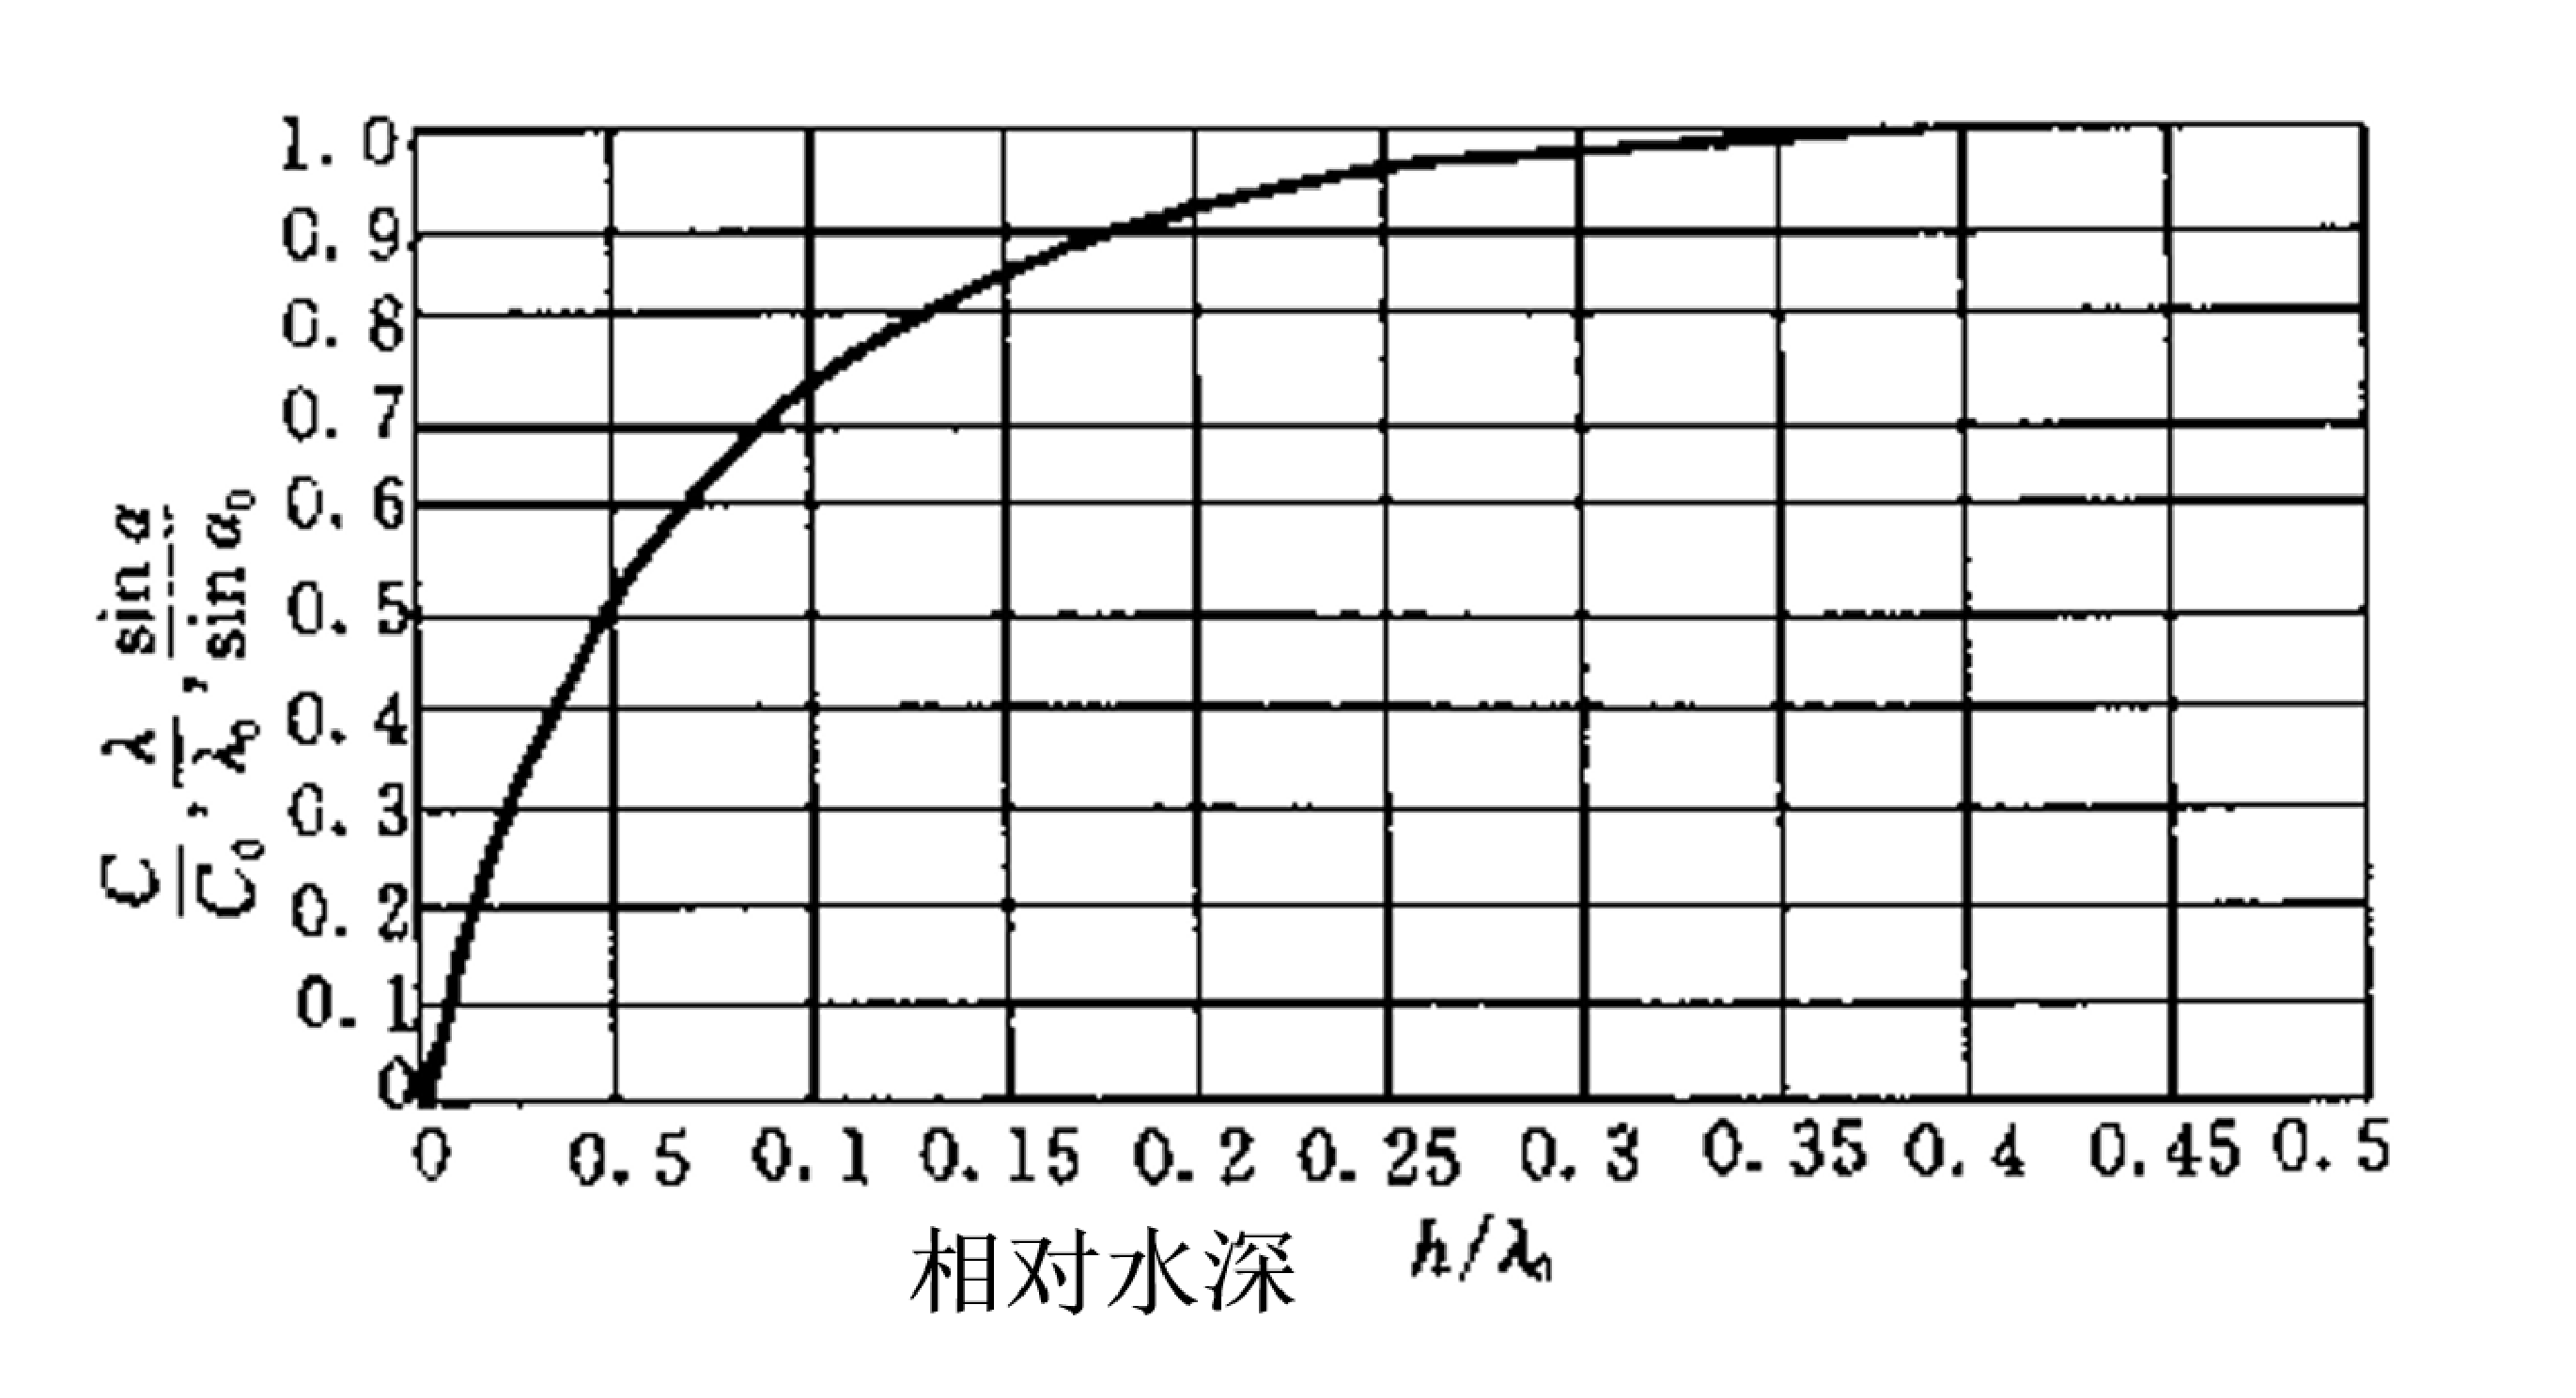
\includegraphics[width=10cm]{23.eps}
    \caption*{}
    \end{figure}
    \paragraph{波向}~{}\\
    波动传播是沿着所需时间最少的路径
    \begin{figure}[H]
    \centering 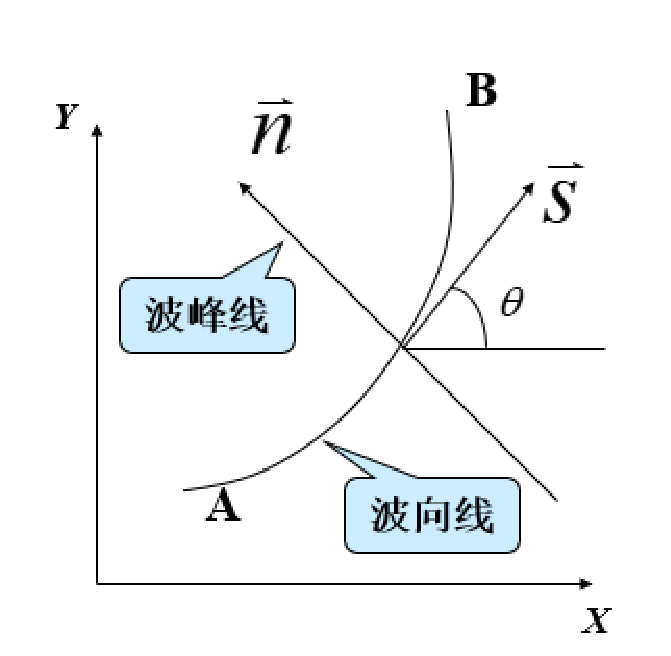
\includegraphics[width=10cm]{24.eps}
    \caption*{}
    \end{figure}
    波峰线从A移动到B所需时间为:
    \[
        t=\int_A^B\frac{ds}{c(x,y)},ds=\sqrt{(d x)^{2}+(d y)^{2}} \Rightarrow d s=\sqrt{1+\left(\frac{d y}{d x}\right)^{2}} d x=\sqrt{1+\left(y^{\prime}\right)^{2}} d x
    \]
    \[
        \Rightarrow t=\int_A^B\frac{\sqrt{1+(y')^2}}{c(x,y)}dx=\int_A^B F(x,y,y')dx
    \]
    使泛函t取极小值的F满足:
    \[
        F_y-\frac{d}{dx}F_{y'}
    \]
    \begin{equation}
        \Rightarrow \frac{y^{\prime \prime}}{1+y^{\prime 2}}=-\frac{1}{c}\left(\frac{\partial c}{\partial y}-y^{\prime} \frac{\partial c}{\partial x}\right)\label{eleq}
    \end{equation}
    由于$y$只与$x$有关:$\displaystyle \frac{\partial y}{\partial x}=\frac{d y}{d x}=\operatorname{tan} \theta$,代入$(\ref{eleq})$:
    \[
        \begin{aligned}
        &\frac{\frac{d\tan \theta}{dx}}{1+\tan^2\theta}=-\frac{1}{c}\left(\frac{\partial}{\partial y}-\tan \theta \frac{\partial}{\partial x}\right)c\\
        \mathop{\Longrightarrow}\limits^{*\cos\theta}& \cos\theta\frac{d\theta}{dx}=-\frac{1}{c}\left(-\cos\theta\frac{\partial}{\partial x}+\sin\theta\frac{\partial}{\partial y}\right)c
        \end{aligned}
    \]
    等式左边由$\displaystyle dx=ds\cos\theta$化为:$\displaystyle \frac{d\theta}{ds}$\\
    等式右边由$\displaystyle \left\langle-\cos\theta,\sin\theta\right\rangle\cdot\nabla c=\hat{n}\cdot\nabla c=\frac{\partial c}{\partial n}\mathop{=}\limits^{\mbox{定常}}\frac{dc}{dn}$化为:$\displaystyle -\frac{1}{c}\frac{dc}{dn}$
    \[
        \Rightarrow \frac{d \theta}{d s}=-\frac{1}{c} \frac{d c}{d n}
    \]
    即波向$\theta$的微分方程.\\
    \[
        \displaystyle c_A>c_B\Rightarrow\frac{dc}{dn}<0\Rightarrow\frac{d\theta}{ds}>0
    \] 
    即$\theta$随$s$越来越大,波向线在浅水趋于与岸线垂直.\\
    \paragraph{波高}~{}\\
    前提:两条波向线间任意断面上的能通量相等.\\
    有限水深的平均能量通量为:$\displaystyle \frac{1}{2}\rho g a^2\cdot \frac{c}{2}\left(1+\frac{2kd}{\mathrm{sh} 2kd}\right)$,其中$H=2a$\\
    因此两条波向线间任意断面上的能通量为:$\displaystyle \frac{1}{8}\rho g H^2\cdot \frac{c}{2}\left(1+\frac{2kd}{\mathrm{sh} 2kd}\right)\cdot l$
    \begin{figure}[H]
        \centering 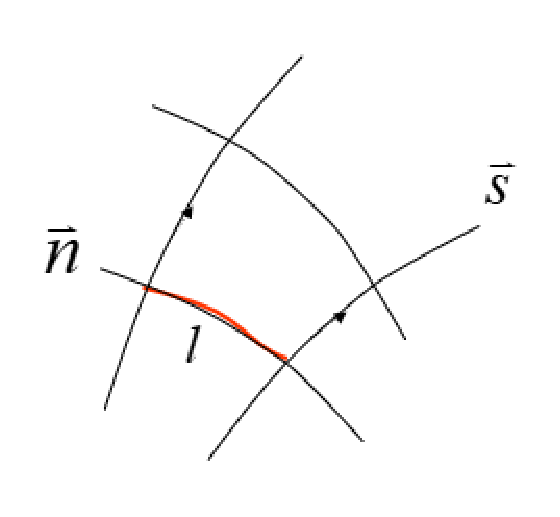
\includegraphics[width=6cm]{25.eps}
        \caption*{}
    \end{figure}
    对于深水:$\displaystyle \bar{P_0}=\frac{1}{8}\rho g H_0^2\frac{c_0}{2}l_0=\bar{P}$
    \[
        \Rightarrow \frac{H}{H_0}=\left(\overbrace{\frac{c_0}{c}\frac{1}{1+\frac{2kd}{\mathrm{sh}2kd}}}^{\mbox{变浅因子D}}\underbrace{\frac{l_0}{l}}_{\mbox{折射因子}}\right)^{\frac{1}{2}}
    \]
    波向线散开因子:$\displaystyle \beta=\frac{l}{l_0}$
    \paragraph{当波浪从深水传入浅水时}~{}\\
    平直海岸,且波向线垂直于岸线,不发生折射,即l=l0,变浅因子起决定作用,波高先略有降低,之后随相对深度的变浅而迅速增大;\\
    海岬处:波向线辐聚$l<l_0$,折射因子大于1,能量集中,波高增大,出现大浪;\\
    海湾处:波向线辐散$l>l_0$,折射因子小于1,能量分散,波高减小,海面较平静.
    \newpage
    \paragraph{总结}~{}
    \begin{figure}[H]
        \centering 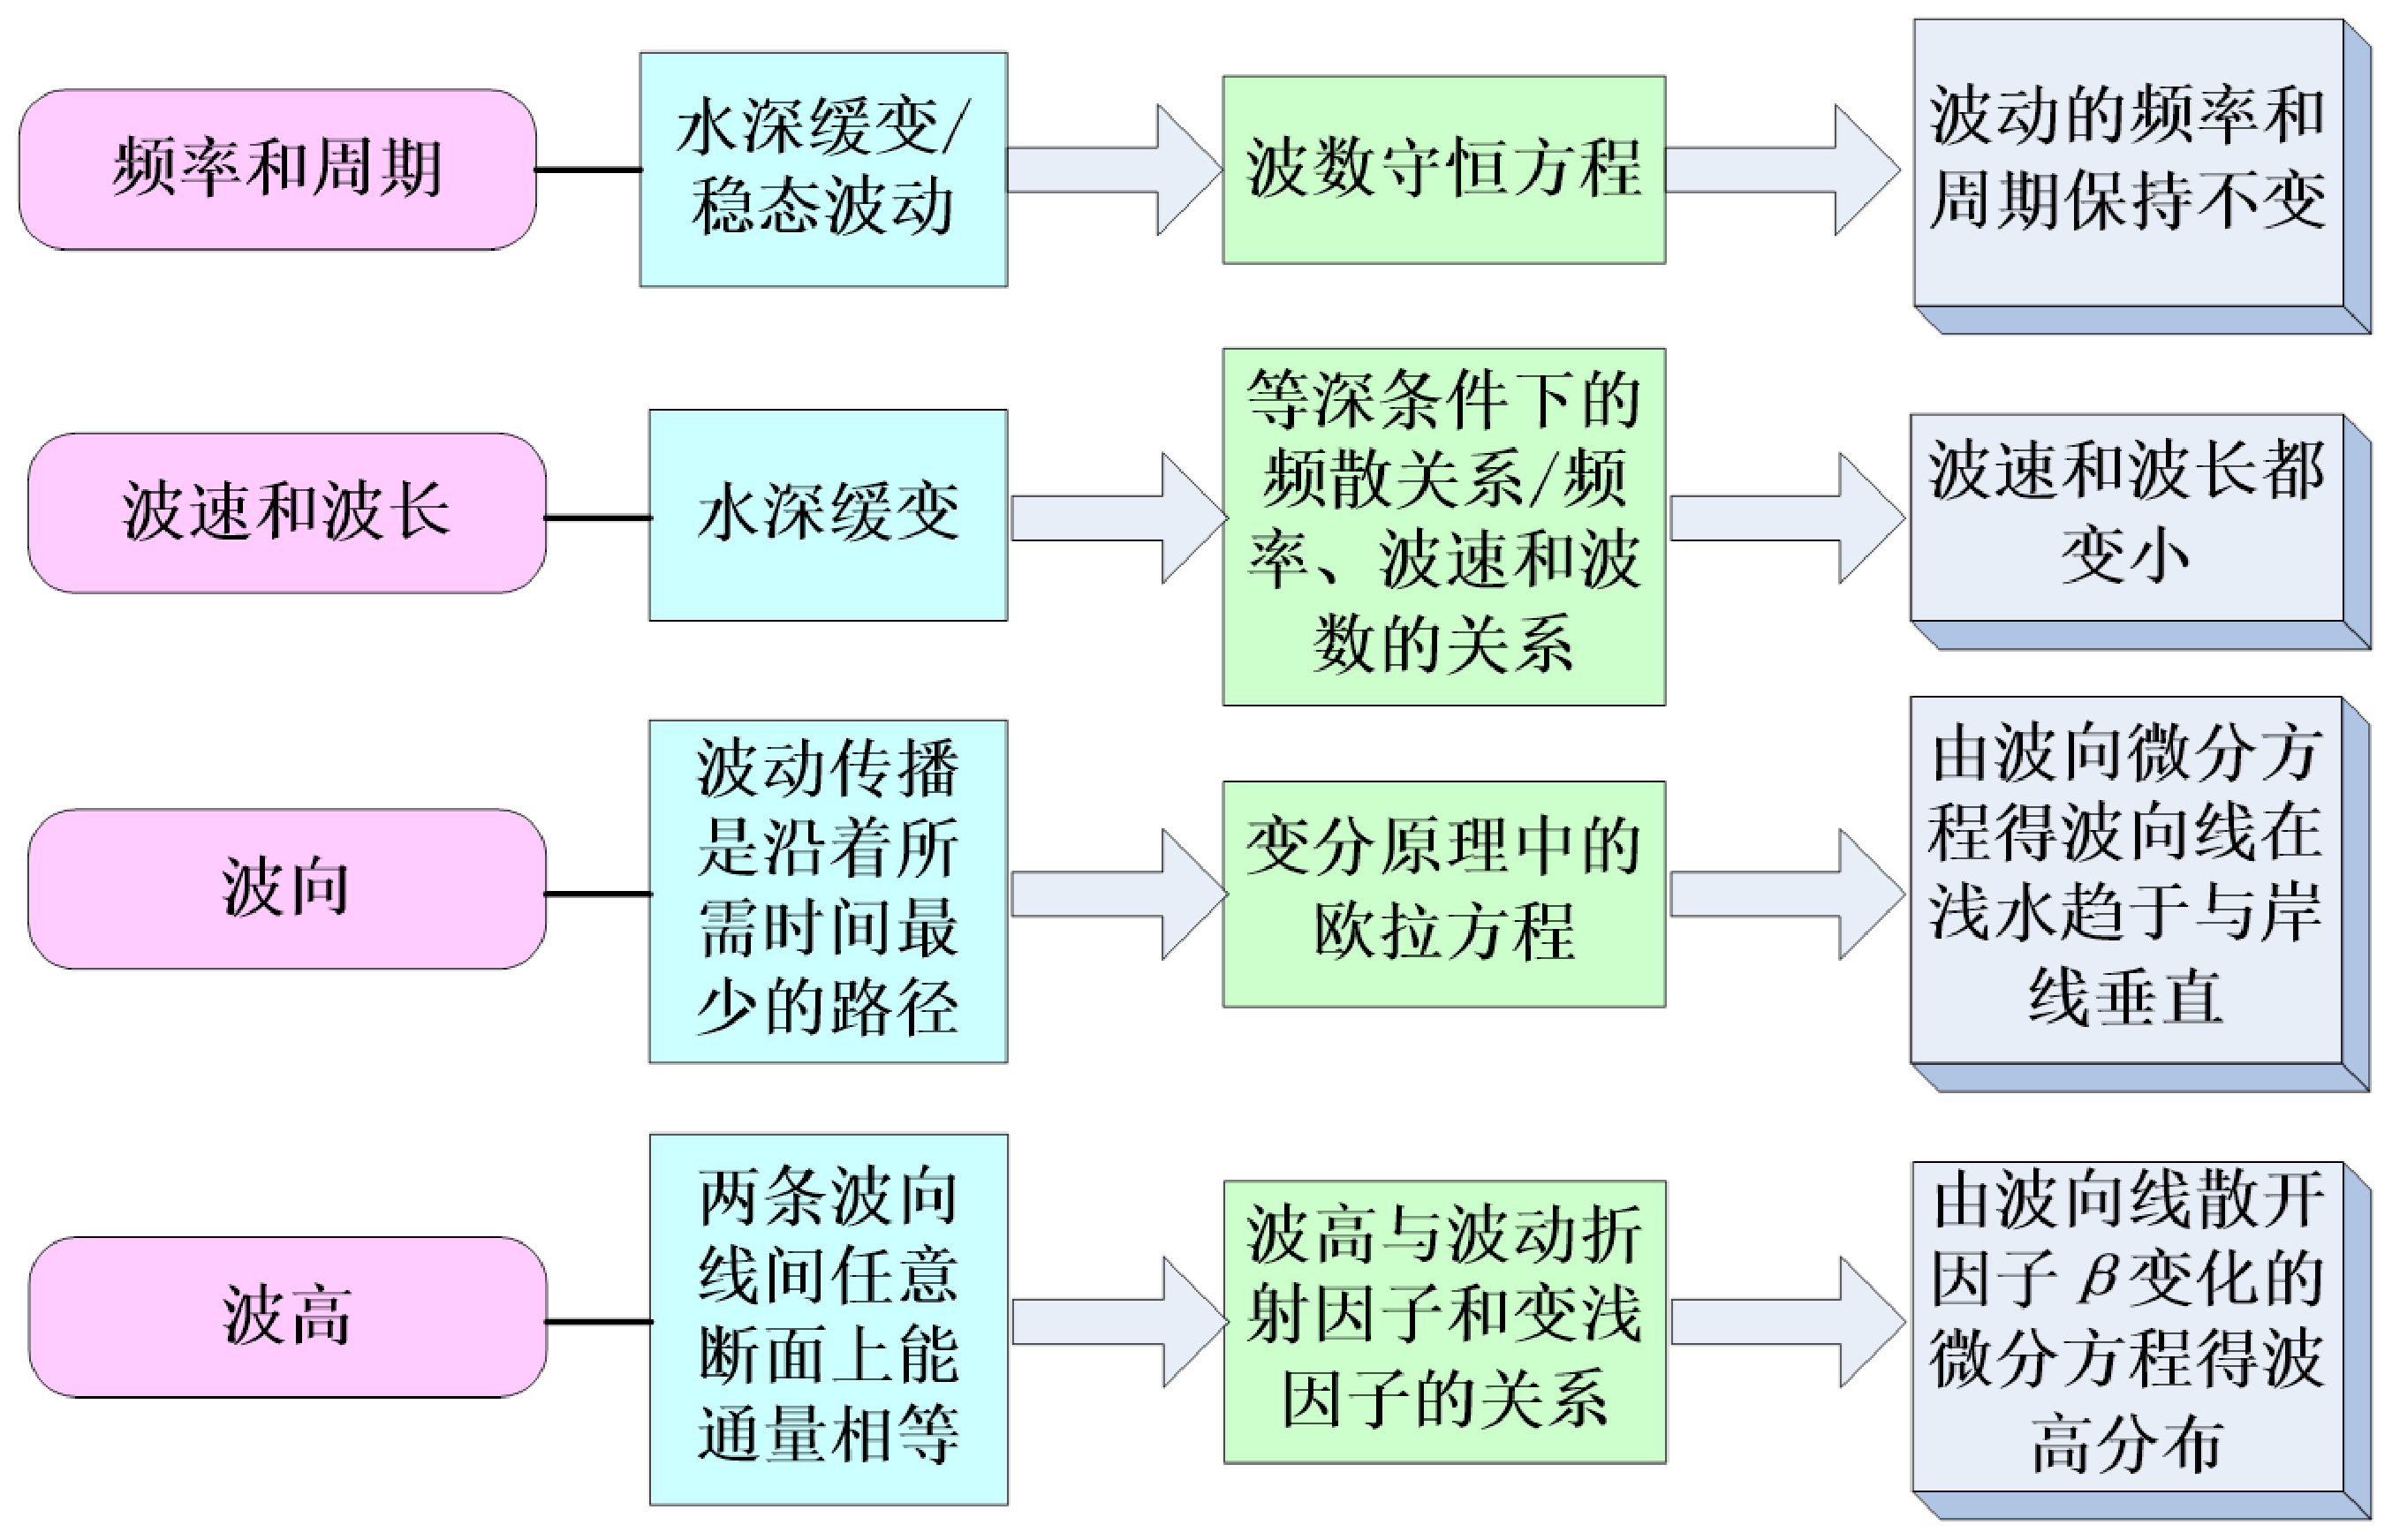
\includegraphics[width=13cm]{27.eps}
        \caption*{}
    \end{figure}
    \subsection{有限振幅波动(不要求掌握)}
    \subsubsection{Stokes波}
    \subsubsection{波浪破碎}
    \paragraph{以深水波为例,分析Stokes波和线性波动的区别和联系}~{}\\
    关联:1阶Stokes波简化为线性波动;\\
    假定:理想波动,没有小振幅的假定;\\
    波面:波面关于x轴不对称,波峰变陡,波谷变平,表面水质点振动中心高于平均静止海面;\\
    波速和频率:与波动振幅 有关,较线性波动略大,且波陡愈大,波速和频率也愈大;\\
    水质点运动轨迹:接近为圆,但在一个周期内不封闭,有净位移,产生波流,存在体积输运;\\
    波浪破碎:波陡达一定限度(1/7)时,波浪就会破碎.
    \subsection{海浪的统计性质}
    \subsubsection{随机海浪过程的基本统计特性}
    \paragraph{平稳性}~{}\\
    广义平稳随机过程:随机过程的数学期望为常量,自协方差只与时间间隔$\tau$有关.\\
    均值(数学期望):$E\{X(t)\}=a$\\
    自相关函数:$E\{X(t+\tau)X(t)\}=R(\tau)$\\
    自协方差函数:$E\{[X(t+\tau)-E\{X(t+\tau)\}][X(t)-E\{X(t)\}]\}=c(\tau)$\\
    方差:$c(0)=DX(t)=E\{[X(t)-E\{X(t)\}]^2\}=\sigma^2$\\
    证明随机海浪过程具有平稳性:\\
    如果实际海浪可以用许多随机的正弦波的叠加来表示,叠加后波面高度的均值为零:$\displaystyle \bar{\zeta}(t)=0$\\
    波面高度的方差,在风浪发展不同阶段不为常数。\\
    但若取很短的时间,方差近似为常数:$\displaystyle \sigma^2(t)=E\{[\zeta(t)-0]^2\}=\overline{\zeta^2(t)}\approx$常数.\\
    对很短时间,海浪随机过程可视为准平稳过程;海浪过程的平稳性保证了记录时间的起点不影响计算结果.\\
    \paragraph{各态历经性}~{}\\
    定义:\\
    设$X(t)$为一平稳随机过程.\\
    若其沿整个时间轴的时间平均值$\left\langle X(t) \right\rangle =E{X(t)}=a$对$X(t)$所有样本函数成立,则该平稳随机过程的均值具有各态历经性;\\
    若其时间平均相关函数$\left\langle X(t)X(t+\tau)\right\rangle=E[X(t)X(t+\tau)]=R(\tau)$对$X(t)$所有样本函数成立,则该平稳随机过程的自相关函数具有各态历经性;\\
    若$X(t)$的均值和自相关函数都具有各态历经性,则该平稳随机过程具有(宽)各态历经性.\\
    \paragraph{证明随机海浪过程具有各态历经性}~{}\\
    根据定义,可以证明:若$X(t)$为各态历经平稳过程,当$|\tau|\rightarrow \infty$时,有$c(\tau)\rightarrow 0$;\\
    自协方差函数$c(\tau)$反映了随机过程中相隔$\tau$的两个随机变量之间的相关程度;\\
    时间间隔较大时,$\zeta(t+\tau)$和$\zeta(t)$的自协方差值很小,可粗略认为:当$\tau\rightarrow\infty$时,$c(\tau)\rightarrow 0$\\
    \begin{framed}
        时间间隔较大时,可认为海浪随机过程满足各态历经性;\\
        各态历经性保证了一次现实可以代替总体;\\
        在实际观测中,一次现实的时间长度T,一般取10~30分钟.
    \end{framed}
    \paragraph{随机海浪过程的正态性}~{}\\
    如果实际海浪可以用许多随机的正弦波动叠加来表示,当$n\rightarrow\infty$时,根据李亚普诺夫定理,波面高度的分布服从正态分布.
    \subsubsection{波面、波高、周期和波长的分布}
    \paragraph{波面的分布}~{}\\
    总的来说,可认为波面高度服从正态分布:
    \[
        f(x)=\frac{1}{\sqrt{2\pi}\sigma}e^{-\frac{(x-a)^2}{2\sigma^2}}
    \]
    \begin{figure}[H]
        \centering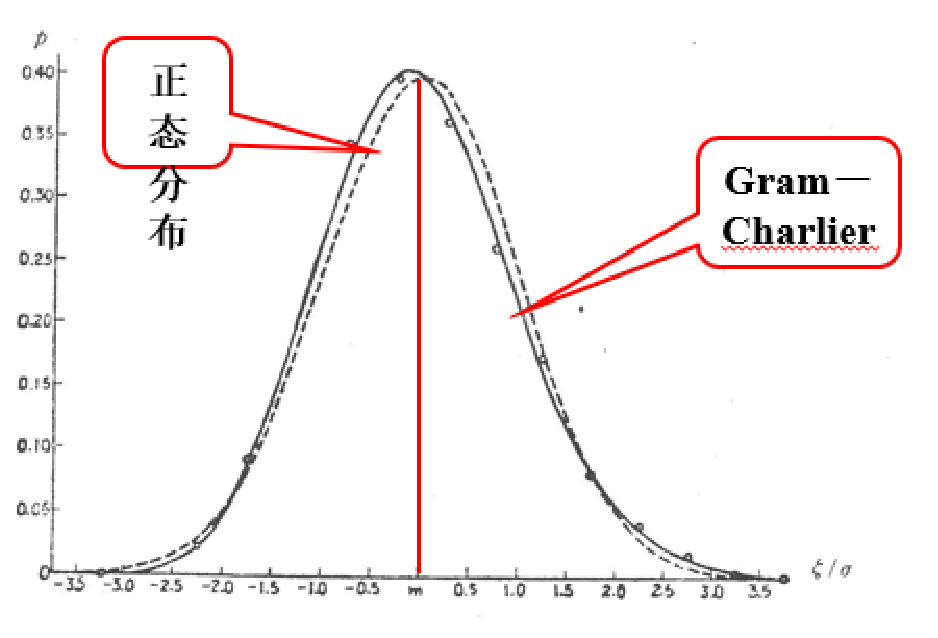
\includegraphics[width=10cm]{28.eps}
        \caption*{}
    \end{figure}
    \paragraph{波高的分布}~{}\\
    随机海浪过程的波高分布为瑞利分布:
    \[
        f(H)=\frac{\pi H}{2\bar{H}^2}e^{-\frac{\pi H^2}{4\bar{H}^2}}
    \]
    在波面高度分布是正态分布的前提下;对窄谱海浪,包络线振幅变化缓慢,可用包络线的纵坐标代表波面的振幅,继而得到波高的分布.
    \begin{figure}[H]
        \centering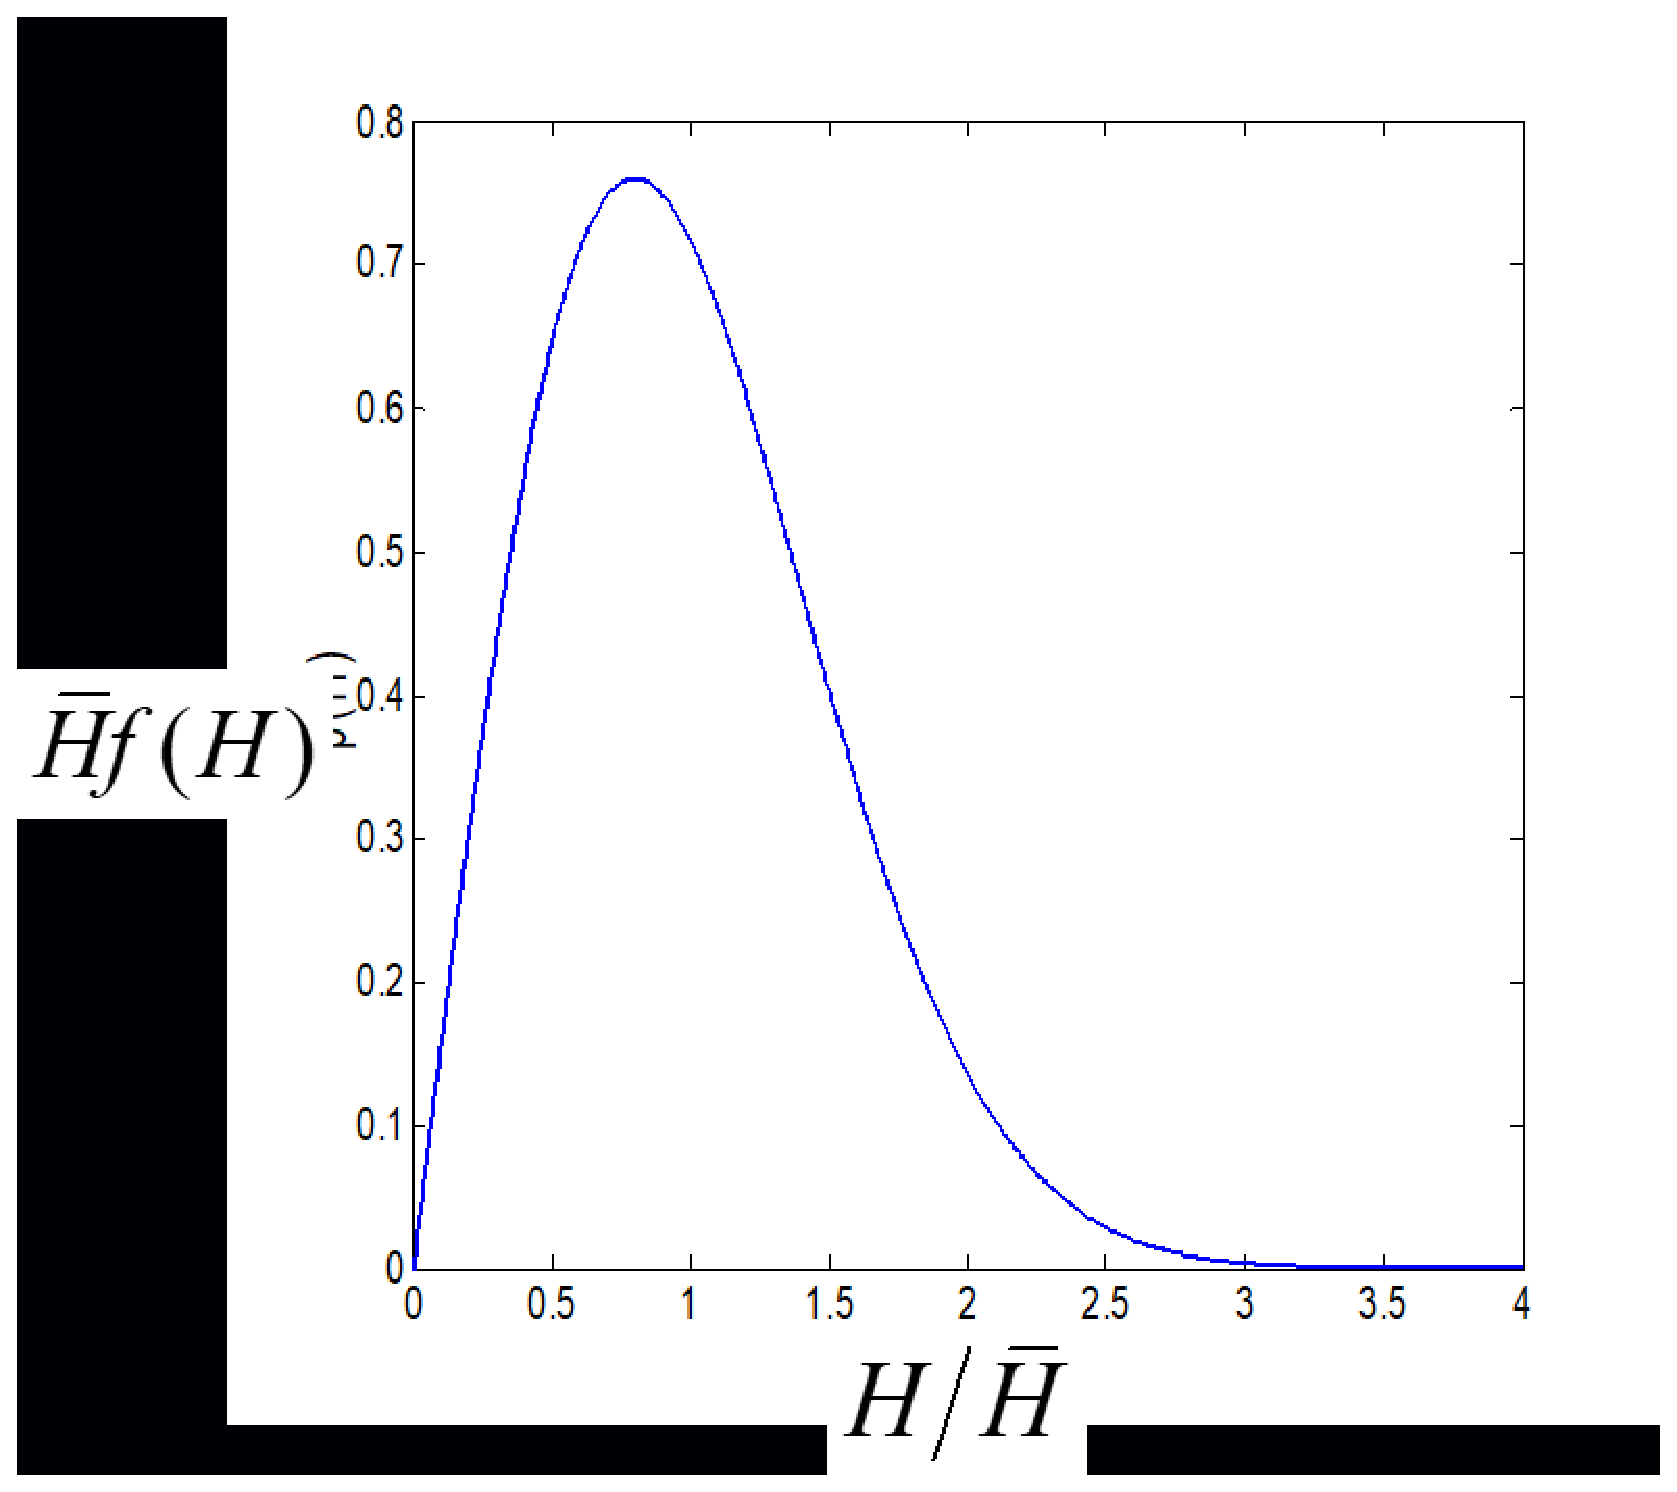
\includegraphics[width=10cm]{29.eps}
        \caption*{}
    \end{figure}
    \paragraph{周期和波长的分布}~{}\\
    随机海浪过程半经验半理论的波长概率密度(瑞利分布):
    \[
        f(\lambda)=\frac{\pi}{2} \frac{\lambda}{\lambda^{2}} \exp \left(-\frac{\pi}{4} \frac{\lambda^{2}}{\bar{\lambda}^{2}}\right)
    \]
    对于深水波:$\displaystyle \lambda=c T=\frac{g}{k c} T=\frac{\lambda g T}{2 \pi \lambda} T=\frac{g T^{2}}{2 \pi}$\\
    周期分布:
    \[
        f(T)=\frac{\pi T^{3}}{T_{0}^{4}} \exp \left(-\frac{\pi}{4} \frac{T^{4}}{T_{0}^{4}}\right),T_{0}=\sqrt{2 \pi \bar{\lambda} / g}
    \]
    观测表明:波浪由深水进入浅水,周期几乎不变,其分布与水深无关,其但波长随水深改变,分布也随水深而变.
    \paragraph{各种波高之间的关系}~{}\\
    1. 均方根波高与平均波高:$\displaystyle H_{rms}=\frac{2}{\sqrt{\pi}}\bar{H}=1.129\bar{H}$\\
    2. 累积率波高与平均波高:$\displaystyle \frac{H_{F}}{\bar{H}}=\left(\frac{4}{\pi} \ln \frac{1}{F}\right)^{1 / 2}$\\
    3. 大波平均波高与平均波高:$\displaystyle \frac{H_{p}}{\bar{H}}=\frac{\sqrt{\pi}}{2}\left(\ln \frac{1}{p}\right)^{1 / 2}+\frac{1}{p}\left\{1-\operatorname{erf}\left[\left(\ln \frac{1}{p}\right)^{1 / 2}\right]\right\},\frac{H_{1 / 3}}{\bar{H}}=1.596$\\
    4. 最大可能波高与平均波高:$\displaystyle H_{\mathrm{m}}=\sqrt{\frac{2}{\pi}} \bar{H} \approx 0.8 \bar{H}$\\
    \subsection{海浪谱}
    \subsubsection{能谱}~{}\\
    观测到的波面可写为:
    \[
        \zeta(t)=\sum_{i=1}^{n} a_{i} \cos \left(\omega_{i} t+\varepsilon_{i}\right)
    \]
    方差之和为:
    \[
        \sigma^{2}=\sum_{i=1}^{n} \sigma^{2}(i)=\frac{1}{2} \sum_{i=1}^{n} a_{i}^{2}
    \]
    回顾$\ref{energy}$,波动平均总能量为:
    \[
        \bar E = {1 \over 2}\rho g{a^2}
    \]
    总方差正比于组成波的总能量,不同频率$\displaystyle \omega_i$对应着不同的$\displaystyle \sigma^2(i)$,即对应着不同组成波的能量.\\
    如果$\omega$近似连续分布,对任意小的频率区间,总对应着一个组成方差的部分和:
    \[
        \Delta \sigma^{2}=\sum_{\omega_{k}-\Delta \omega / 2}^{\omega_{k}+\Delta \omega / 2} \sigma^{2}\left(\omega_{k}\right)
    \]
    能谱定义为:
    \[
        S(\omega_k)=\frac{\Delta \sigma^{2}=\sum_{\omega_{k}-\Delta \omega / 2}^{\omega_{k}+\Delta \omega / 2} \sigma^{2}\left(\omega_{k}\right)}{\Delta \omega}
    \]
    它比例于一段频率范围内组成波能量之和的平均.\\
    当$n$很大时:
    \[
        \sigma^{2}=\sum_{i=1}^{n} \sigma^{2}(i) \Rightarrow \sigma^{2}=\sum_{k=1}^{\infty} S\left(\omega_{k}\right) \Delta \omega \Rightarrow \sigma^{2}=\int_{0}^{\infty} S(\omega) d \omega
    \]
    即能谱的积分等于总方差.\\
    由协方差确定能谱:
    \[
        \begin{aligned}
            R(\tau)&=E\{\zeta(t)\zeta(t+\tau)\}\\
            &=\sum_{i=1}^{\infty}\frac{1}{2}a_i^2\cos (\omega_i \tau)\\
            &=\sum_{i=1}^{\infty} \sigma^{2}(i) \cos \left(\omega_{i} \tau\right)\\
            &=\sum_{i=1}^{\infty} S\left(\omega_{i}\right) \delta \omega \cos \left(\omega_{i} \tau\right)\\
            (\mbox{取极限})&=\int_{0}^{\infty} S(\omega) \cos (\omega \tau) d \omega\\
            (\mbox{傅里叶变换})&\Rightarrow \underbrace{S(\omega)=\frac{2}{\pi} \int_{0}^{\infty} R(\tau) \cos \omega \tau d \tau}_{\mbox{能谱的基本表达式}}
        \end{aligned}
    \]
    \subsubsection{方向谱}~{}\\
    海浪能量相对于频率和方向的分布.
    \[
        \zeta(x, y, t)=\sum^{\infty}_{n=0} a_{n} \cos \left(l_{n} x+m_{n} y-\omega_{n} t+\varepsilon_{n}\right)
    \]
    \[
        \begin{aligned}
            &S(l,m) = {{\sum\limits_{l - \Delta l/2}^{l +\Delta l/2} {\sum\limits_{m - \Delta m/2}^{m +\Delta m/2} {{1 \over 2}a_n^2} } } \over {\Delta l \Delta m}}\\
            &S(\omega ,\theta ) = {{\sum\limits_{\omega  -\Delta \omega /2}^{\omega  +\Delta \omega /2} {\sum\limits_{\theta  -\Delta \theta /2}^{\theta  +\Delta \theta /2} {{1 \over 2}a_n^2} } } \over {\Delta \omega \Delta \theta }}
        \end{aligned}
    \]
    方向谱不仅能反映海浪内部的频率结构,还能够反映海浪内部的方向结构.\\
    能谱和方向谱的关系:
    \[
        S(\omega ) = \int_0^{2\pi } {S(\omega ,\theta )d\theta } 
    \]
    \section{潮波}
    \subsection{平衡潮理论}
    \subsubsection{基本假设}
    \begin{figure}[H]
        \centering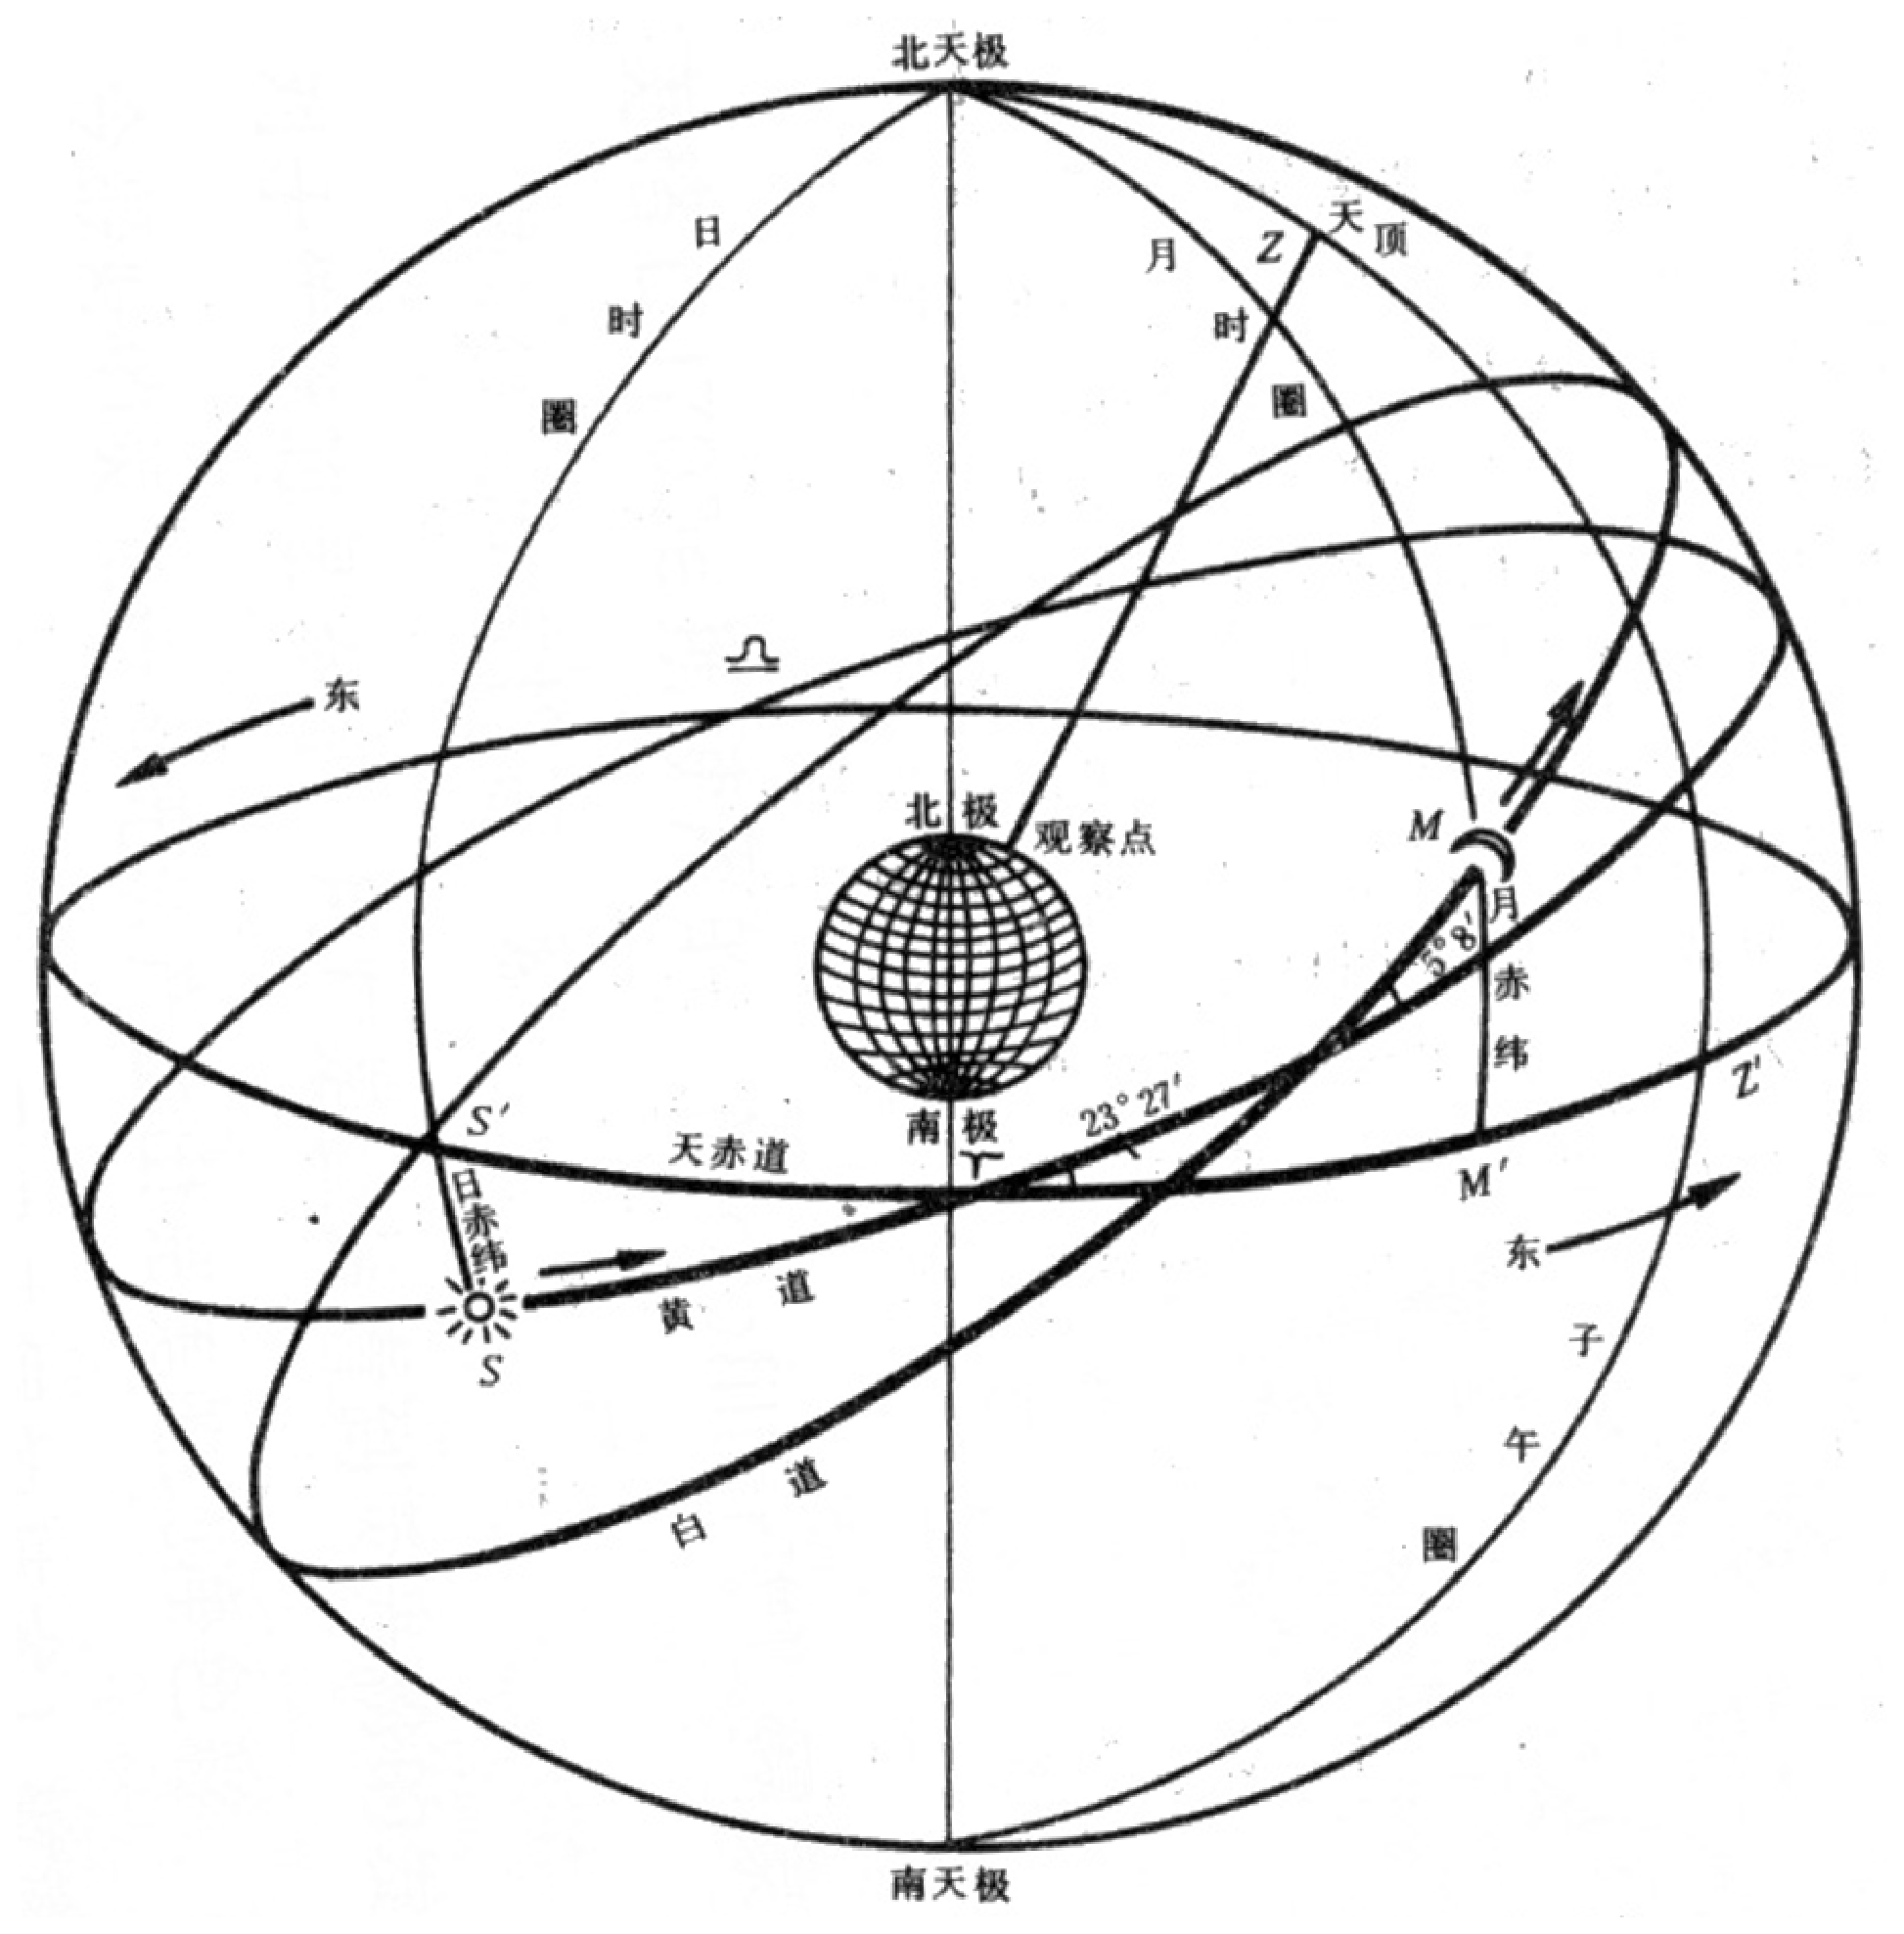
\includegraphics[width=10cm]{30.eps}
        \caption*{}
    \end{figure}
    地球为一圆球,被等深海水覆盖;
    不考虑海水运动,只考虑受力平衡;
    不受地转偏向力和摩擦力作用;\\
    海水无粘性,无惯性;\\
    海面能随时与等势面重叠.\\
    每一瞬间海面都与水平引潮力和重力的合力方向垂直,
    随着天体位置的变化,新的平衡不断取代旧的平衡,达到一种$\color{red}\mbox{动态的静力平衡}$。
    \subsubsection{天体引潮力的主要部分}
    \paragraph{月球引潮力}~{}
    \begin{figure}[H]
        \centering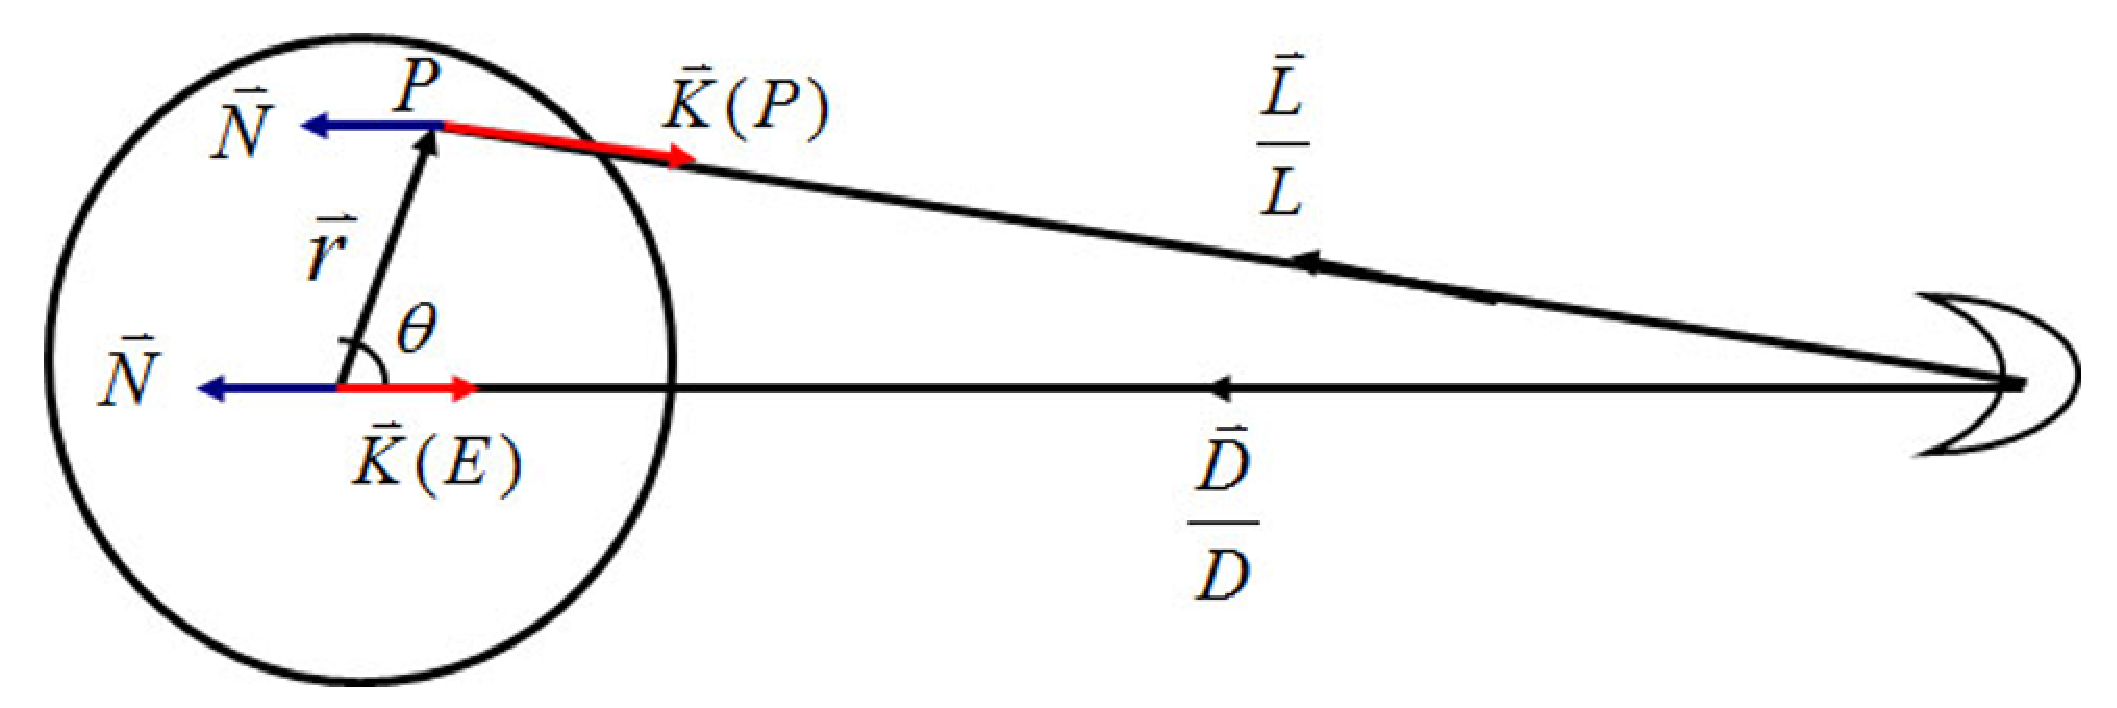
\includegraphics[width=10cm]{31.eps}
        \caption*{}
    \end{figure}
    其中,$\theta$为天顶距.\\
    \begin{table}[htbp]
        \centering 
        \caption*{}
        \begin{tabular}{lll}
            \toprule
            & 对于任意一点$X$ & 对地球质心$E$ \\
            \midrule
        月球引力      &     $\displaystyle \vec{K}(X)=-\mu_0 \frac{M}{L^{2}}\left(\frac{\vec{L}}{L}\right)$     &  $\displaystyle\vec{K}(E)=-\frac{\mu_0 M}{D^{2}}\left(\frac{\vec{D}}{D}\right)$        \\
        公转惯性离心力 &    $\displaystyle\vec{N}=\frac{\mu_0 M}{D^{2}}\left(\frac{\vec{D}}{D}\right)$       &      $\displaystyle\vec{N}=\frac{\mu_0 M}{D^{2}}\left(\frac{\vec{D}}{D}\right)$    \\
        引潮力        &    $\displaystyle\vec{F}_{M}=\vec{N}+\vec{K}(X)$       &    $\displaystyle\vec{F}_{M}=\vec{N}+\vec{K}(E)=0$ \\
        \bottomrule
        \end{tabular}
    \end{table}
    \paragraph{引潮势}~{}\\
    从地心移动单位质量物体到地表某一点,克服引潮力所作的功。引潮力和引潮势的关系:$\vec{F}=-\nabla \varphi$\\
    对$P$点,单位质量所受的月球引力的势:
    \[
        \varphi_{1}=-\int \vec{K}(p) \cdot d \vec{L}=\int K \frac{M}{L^{2}}\left(\frac{\vec{L}}{L}\right) \cdot d \vec{L}=-K \frac{M}{L}+c_{1}
    \]
    设地心处的势为0,则:$\displaystyle \varphi_{1}=-K M\left(\frac{1}{L}-\frac{1}{D}\right)$\\
    对$P$点,单位质量所受的惯性离心力的势:
    \[
        \varphi_{2}=-\int \vec{N} \cdot d \vec{r}=-\int K \frac{M}{D^{2}}\left(\frac{\vec{D}}{D}\right) \cdot d \vec{r}=K \frac{M}{D^{2}} r \cos \theta+c_{2}
    \]
    设地心处的势为0,则:$\displaystyle \varphi_{2}=K \frac{M}{D^{2}} r \cos \theta$
    对$P$点,单位质量所受的月球引潮势:
    \[
        {\varphi _M} = {\varphi _1} + {\varphi _2} =  - K{M}({1 \over L} - {1 \over D}) + K{{{M}} \over {{D^2}}}r\cos \theta  =  - K{M}({1 \over L} - {1 \over D} - {r \over {{D^2}}}\cos \theta )
    \]
    对$P$点,单位质量所受的太阳引潮势:
    \[
        \varphi_{S}=-K M_{S}\left(\frac{1}{L_{S}}-\frac{1}{D_{S}}-\frac{r}{D_{S}^{2}} \cos \theta_{S}\right)
    \]
    天体引潮势:$\displaystyle \varphi_T=\varphi_M+\varphi_S$\\
    天体引潮力:$\displaystyle \vec{F}_T=-\nabla\varphi_T$\\
    根据余弦定理:
    \[
        \begin{aligned}
           {L^2} &= {D^2} + {r^2} - 2Dr\cos \theta  \\
           &=  {D^2}[1 - 2({r \over D})\cos \theta  + {({r \over D})^2}]\\
            \Rightarrow {1 \over L} &= {1 \over D}{[1 - 2({r \over D})\cos \theta  + {({r \over D})^2}]^{ - 1/2}}
        \end{aligned}
    \]
    根据泰勒展开:$\displaystyle {(1 + x)^\mu } = 1 + \mu x + {1 \over {2!}}\mu (\mu  - 1){x^2} + ... + {1 \over {n!}}\mu (\mu  - 1)\cdots (\mu  - n + 1){x^n} + ...$\\
    由于$r\ll D$,把$\displaystyle \frac{r}{D}$看作无穷小量:
    \[
        \begin{aligned}
            \Rightarrow {1 \over L} &= {1 \over D}{[1 - 2({r \over D})\cos \theta  + {({r \over D})^2}]^{ - 1/2}}\\
            &= \frac{1}{D}\left\{1-\frac{1}{2}\left[\left(\frac{r}{D}\right)^2-2\left(\frac{r}{D}\right)\cos\theta\right]+\frac{1}{2}\cdot\left(-\frac{1}{2}\right)\cdot\left(-\frac{3}{2}\right)\left[\left(\frac{r}{D}\right)^2-2\left(\frac{r}{D}\right)\cos\theta\right]^2+o\left[\left(\frac{r}{D}\right)^3\right] \right\}\\
            &= \frac{1}{D}\left\{1-\frac{1}{2}\left(\frac{r}{D}\right)^2+\left(\frac{r}{D}\right)\cos\theta+\frac{3}{8}\cdot 4\left(\frac{r}{D}\right)^2\cos^2\theta +o\left[\left(\frac{r}{D}\right)^3\right]\right\}\\
            &=\frac{1}{D}-\frac{r^2}{2D^3}+\frac{r}{D^2}\cos\theta+\frac{3r^2}{2D^3}\cos^2\theta+o\left(\frac{r^3}{D^4}\right)
        \end{aligned}
    \]
    代入月球引潮势:
    \[
        \begin{aligned}
            {\varphi _M} &=  - {\mu _0}M\left({1 \over L} - {1 \over D} - {r \over {{D^2}}}\cos \theta \right)\\
            &= - {\mu _0}M\left[\frac{1}{D}-\frac{r^2}{2D^3}+\frac{r}{D^2}\cos\theta+\frac{3r^2}{2D^3}\cos^2\theta+o\left(\frac{r^3}{D^4}\right) - {1 \over D} - {r \over {{D^2}}}\cos \theta \right]\\
            &= - {\mu _0}M\left[-\frac{r^2}{2D^3}+\frac{3r^2}{2D^3}\cos^2\theta \right]+o\left(\frac{r^3}{D^4}\right)\\
            &= - {\mu _0}M{{{r^2}} \over {2{D^3}}}(3{\cos ^2}\theta  - 1)+o\left(\frac{r^3}{D^4}\right)\\
            &= V_M+o\left(\frac{r^3}{D^4}\right)
        \end{aligned}
    \]
    $\displaystyle V_M$即月球引潮势的主要部分.
    \paragraph{月球引潮力的铅直和水平分量}~{}
    \[
        \left\{
            \begin{aligned}
               {F_{MV}} &=  - {{\partial {V_M}} \over {\partial r}} = {\mu _0}M{r \over {{D^3}}}(3{\cos ^2}\theta  - 1)\\
               {F_{MH}} &=  - {1 \over r}{{\partial {V_M}} \over {\partial \theta }} =  - {3 \over 2}{\mu _0}M{r \over {{D^3}}}\sin 2\theta
            \end{aligned}
        \right.
    \]
    地球表面单位质量物体受地心引力为:$\displaystyle g=\frac{\mu_0 E}{a^2},r\rightarrow a$\\
    \[
        \left\{
            \begin{aligned}
              {F_{MV}} &= g{{{a^3}} \over {{D^3}}}{M \over E}(3{\cos ^2}\theta  - 1) \to {10^{ - 7}}g\\
              {F_{MH}} &=  - {3 \over 2}g{{{a^3}} \over {{D^3}}}{M \over E}\sin 2\theta  \to {10^{ - 7}}g
            \end{aligned}
        \right.
    \]
    形成海洋潮汐潮流运动的真正原动力是引潮力水平分量.
    \paragraph{潮汐椭球}~{}\\
    在近月点,引潮力方向指向月球;\\
    在远月点,引潮力方向背向月球;\\
    地球表面的海水发生辐聚和辐散,海面变成椭球形(潮汐椭球),长轴指向月球中心.
    \begin{figure}[H]
        \centering 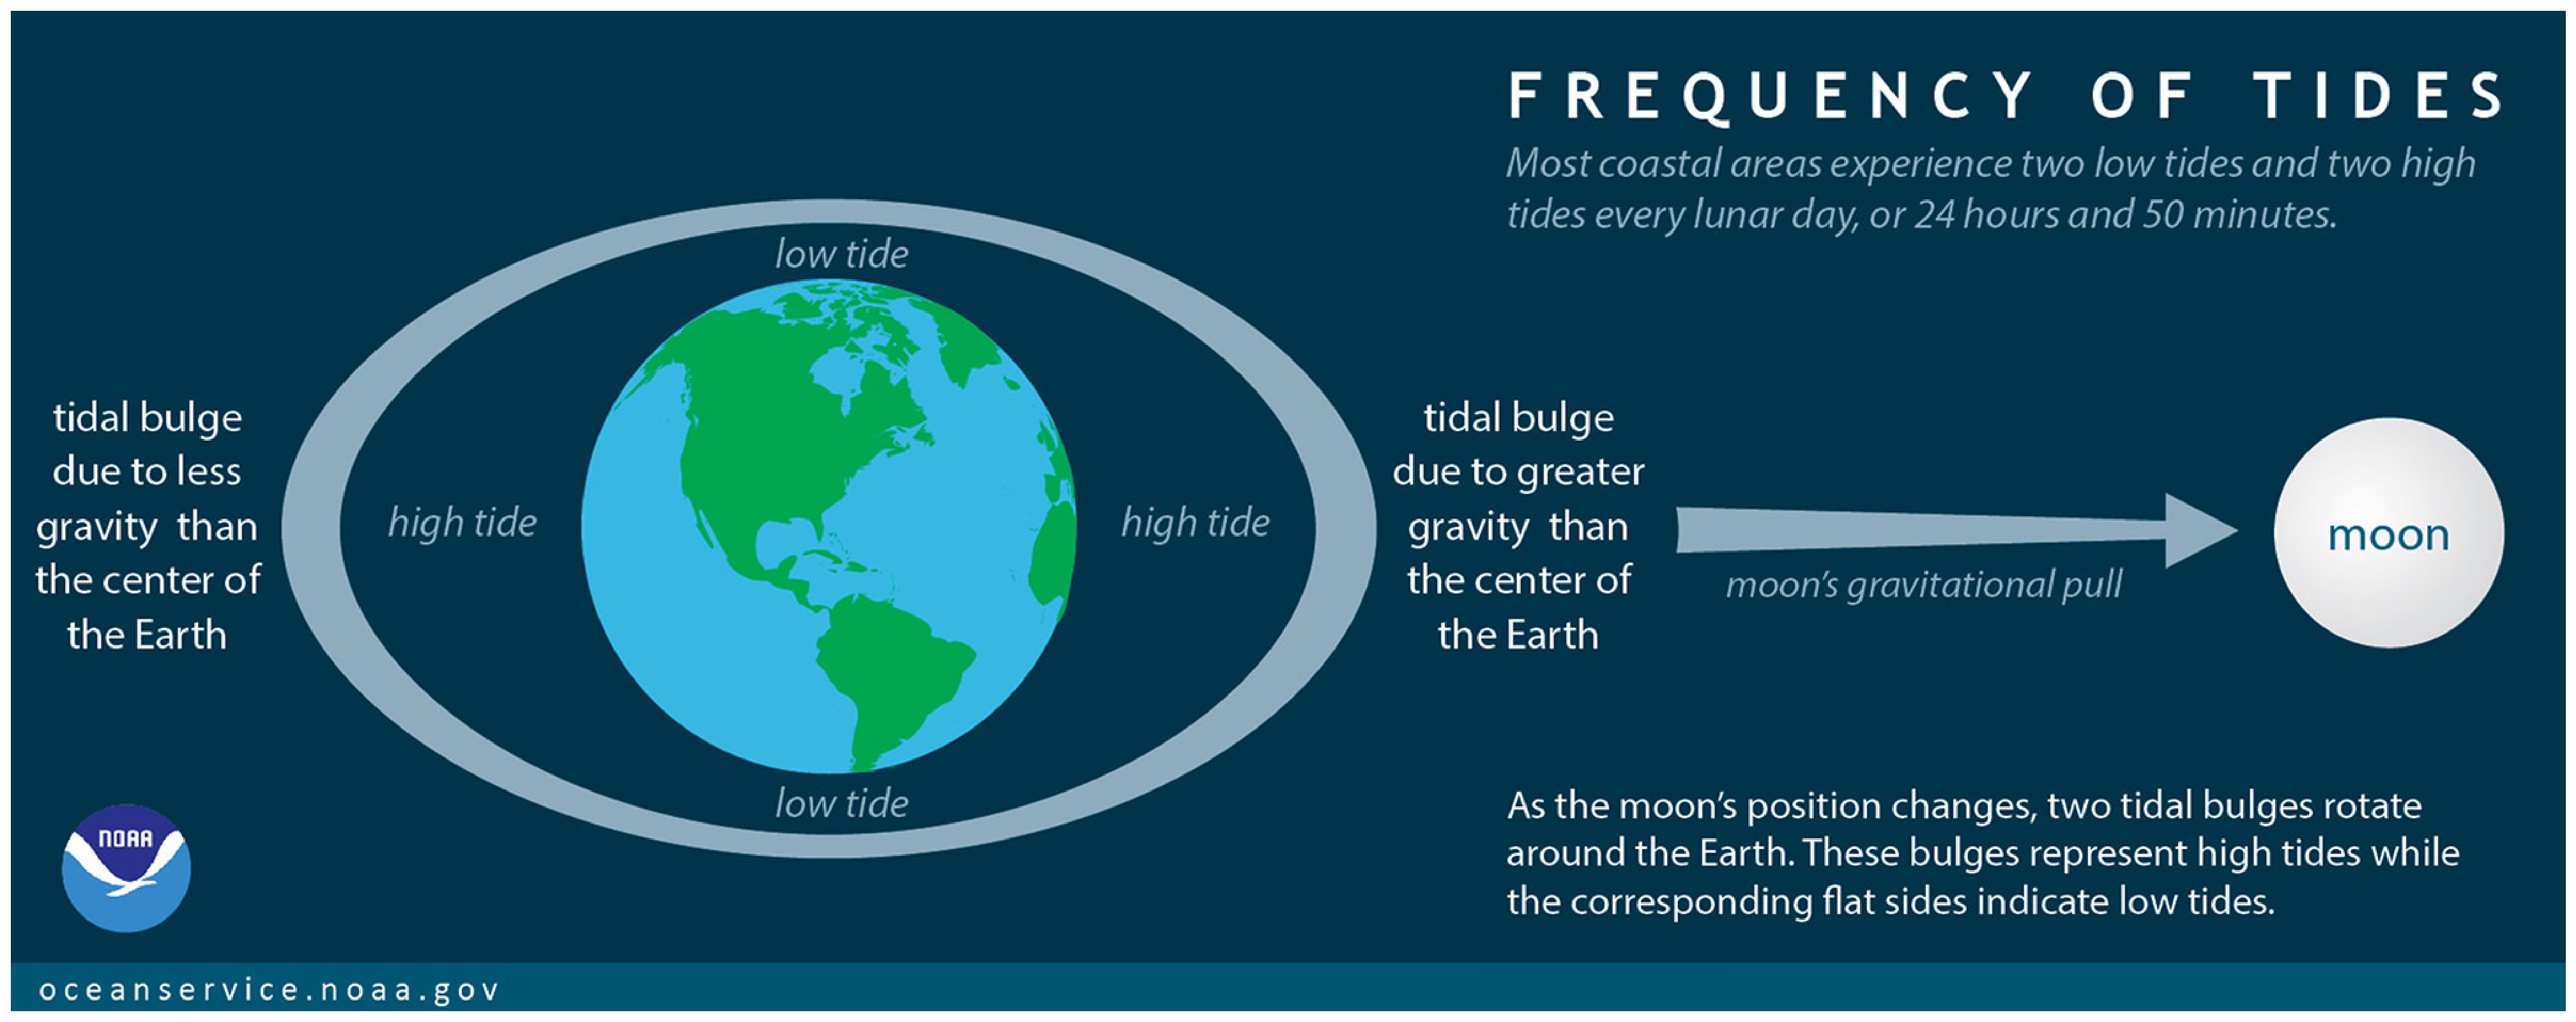
\includegraphics[width=16cm]{33.eps}
        \caption*{\url{https://oceanservice.noaa.gov/facts/tidefrequency.html}}
    \end{figure}
    \subsubsection{平衡潮潮高}~{}\\
    根据平衡潮的概念,某一瞬间海水状态为静力平衡.
    \begin{figure}[H]
        \centering 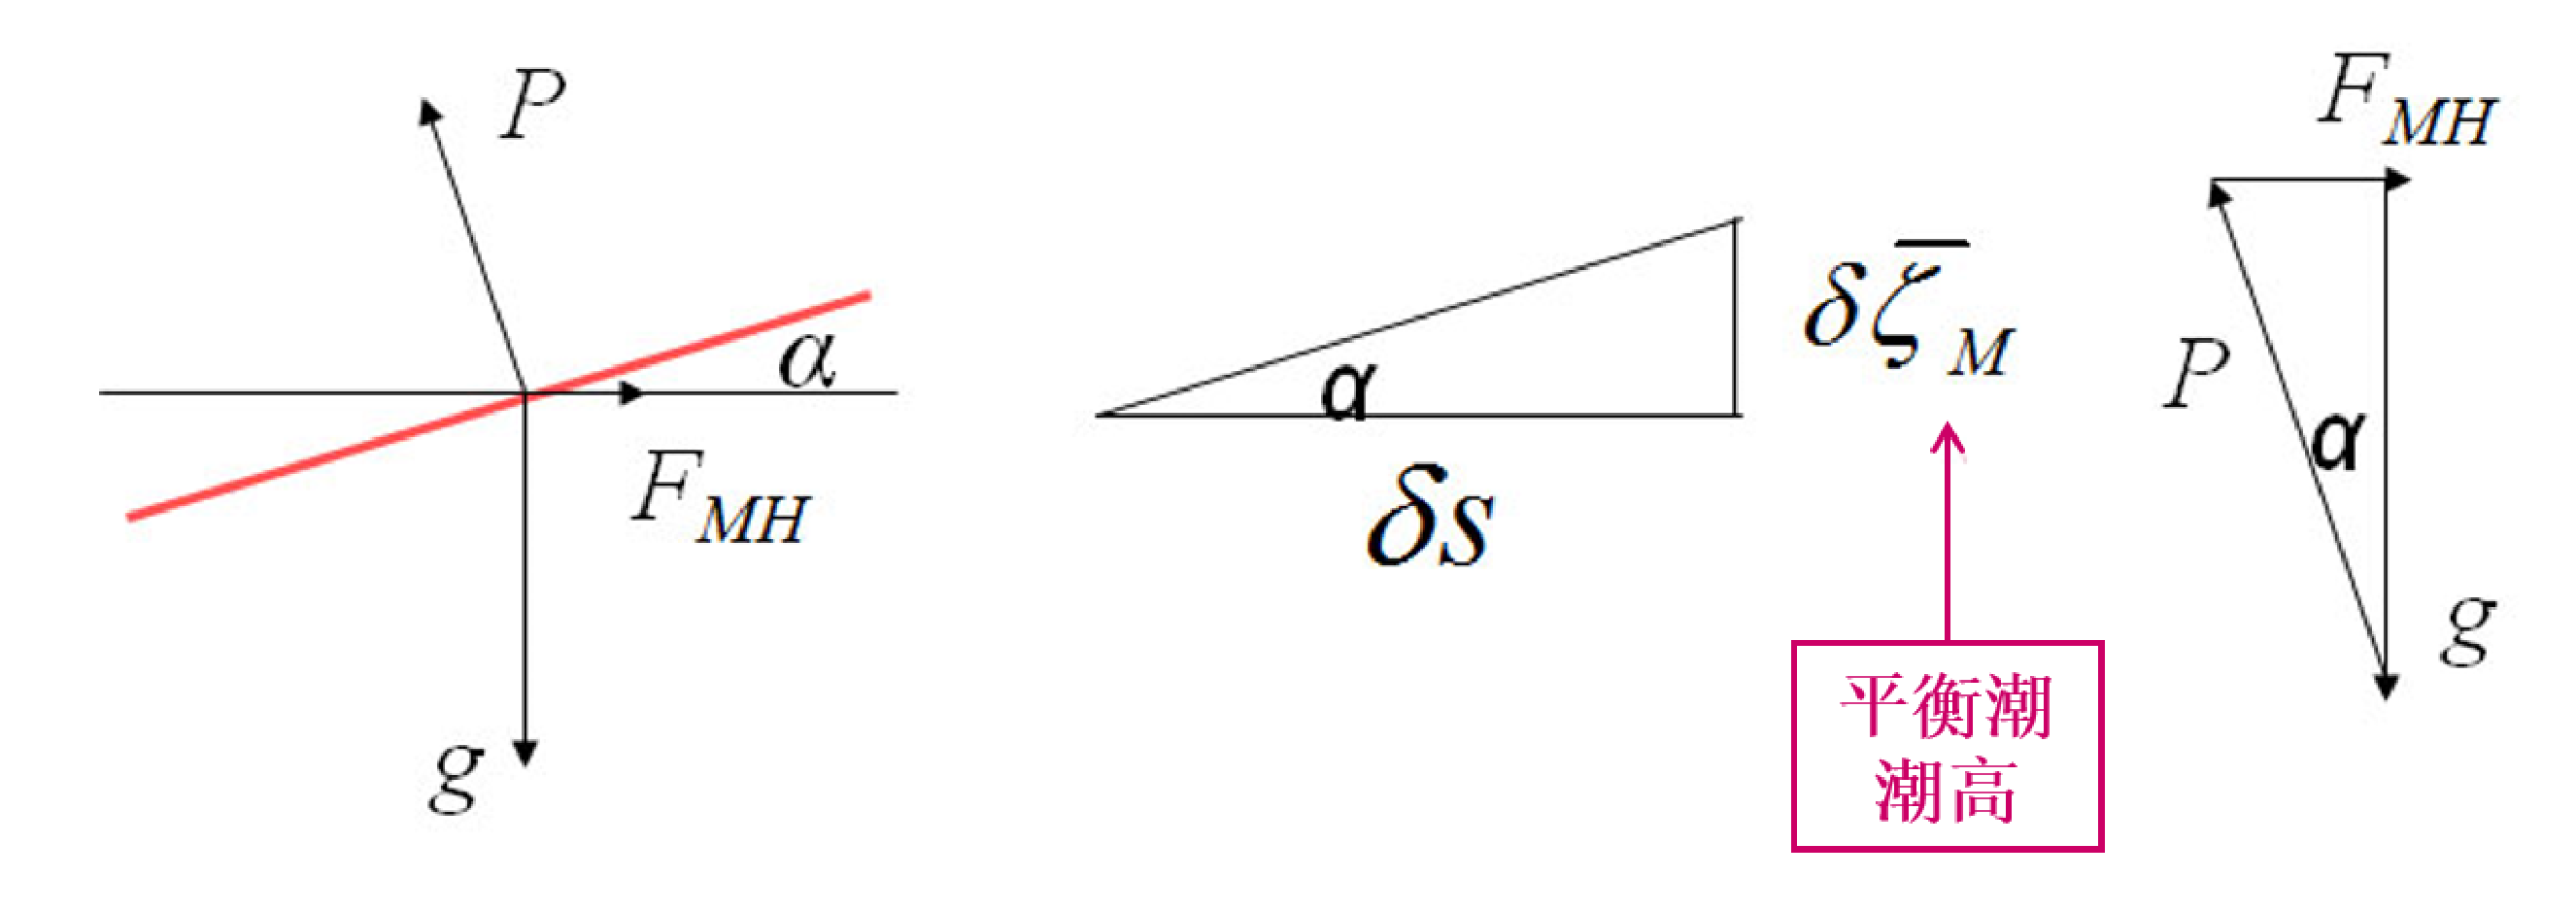
\includegraphics[width=14cm]{34.eps}
        \caption*{}
    \end{figure}
    \[
        \left\{
            \begin{aligned}
                \tan \alpha&={F_{MH} \over g} =\frac{\delta\bar{\zeta}_M}{\delta s}\\
                F_{MH}&=-\frac{\partial V_M}{\partial s}
            \end{aligned}
        \right.
        \Rightarrow \bar{\zeta}_M=-\frac{V_M}{g}+C={{{\mu _0}M} \over g}{{{a^2}} \over {2{D^3}}}(3{\cos ^2}\theta  - 1) + C
    \]
    全球海面升高和降低的水体体积之和为0:
    \begin{figure}[H]
        \centering 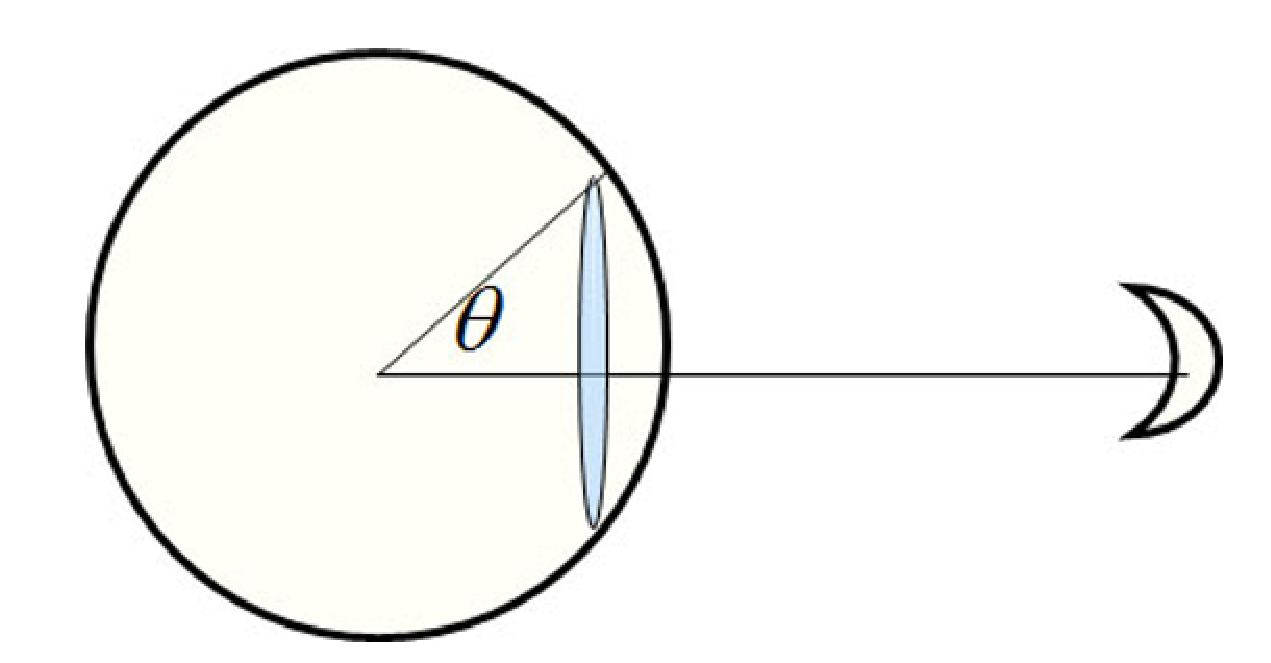
\includegraphics[width=8cm]{35.eps}
        \caption*{积分示意图}
    \end{figure}
    \[
        \int_0^\pi  {{{\bar \zeta }_M} \cdot } 2\pi  \cdot {a^2}\sin \theta d\theta  = 0\Rightarrow C=0
    \]
    代入$\displaystyle g=\frac{\mu_0 E}{a^2}$:
    \[
        {\bar \zeta _M} =  - {{{V_M}} \over g} = {1 \over 2}{M \over E}{({a \over D})^3}a(3{\cos ^2}\theta  - 1)
    \]
    \paragraph{平衡潮最大潮差的估算}~{}\\
    高潮:$\displaystyle {\bar \zeta _{M\max }} = {M \over E}{({a \over D})^3}a,\theta  = 0^\circ/180^\circ$\\
    低潮:$\displaystyle{\bar \zeta _{M\min }} =  - {1 \over 2}{M \over E}{({a \over D})^3}a,\theta  = 90^\circ/270^\circ$\\
    月球平衡潮最大潮差:$\displaystyle {\bar \zeta _{M\max }} - {\bar \zeta _{M\min }} = {3 \over 2}{M \over E}{({a \over D})^3}a = 0.535m$\\
    太阳平衡潮最大潮差:$\displaystyle {\bar \zeta _{S\max }} - {\bar \zeta _{S\min }} = {3 \over 2}{S \over E}{({a \over {{D_s}}})^3}a = 0.246m$\\
    平衡潮最大潮差为78cm.
    \paragraph{平衡潮潮高展开和平衡潮周期}~{}
    \[
        \cos \theta  = \sin \varphi \sin \delta  + \cos \varphi \cos \delta \cos {T_1}
    \]
    \[
        \begin{aligned}
            {{\bar \zeta }_M} &= {{\bar \zeta }_0} + {{\bar \zeta }_1} + {{\bar \zeta }_2}\\
            &= 2G{\left( {{{\bar D} \over D}} \right)^3}\{[ \underbrace{{3 \over 2}({{\sin }^2}\varphi  - {1 \over 3})({{\sin }^2}\delta  - {1 \over 3})}_{\mbox{半回归月周期}} ]  +\underbrace{ {1 \over 2}\sin 2\varphi \sin 2\delta \cos {T_1}}_{\mbox{全太阴日周期}} + \underbrace{{1 \over 2}{\cos ^2}\varphi {\cos ^2}\delta \cos 2T_1}_{\mbox{半太阴日周期}}\}
        \end{aligned}
    \]
    \paragraph{潮汐日不等}~{}\\
    赤纬为0:正规半日潮\\
    赤纬不为0:\\
    赤道:正规半日潮;\\
    极区:正规日潮(极点无潮);\\
    其他区域:日不等现象.\\
    \begin{figure}[H]
        \centering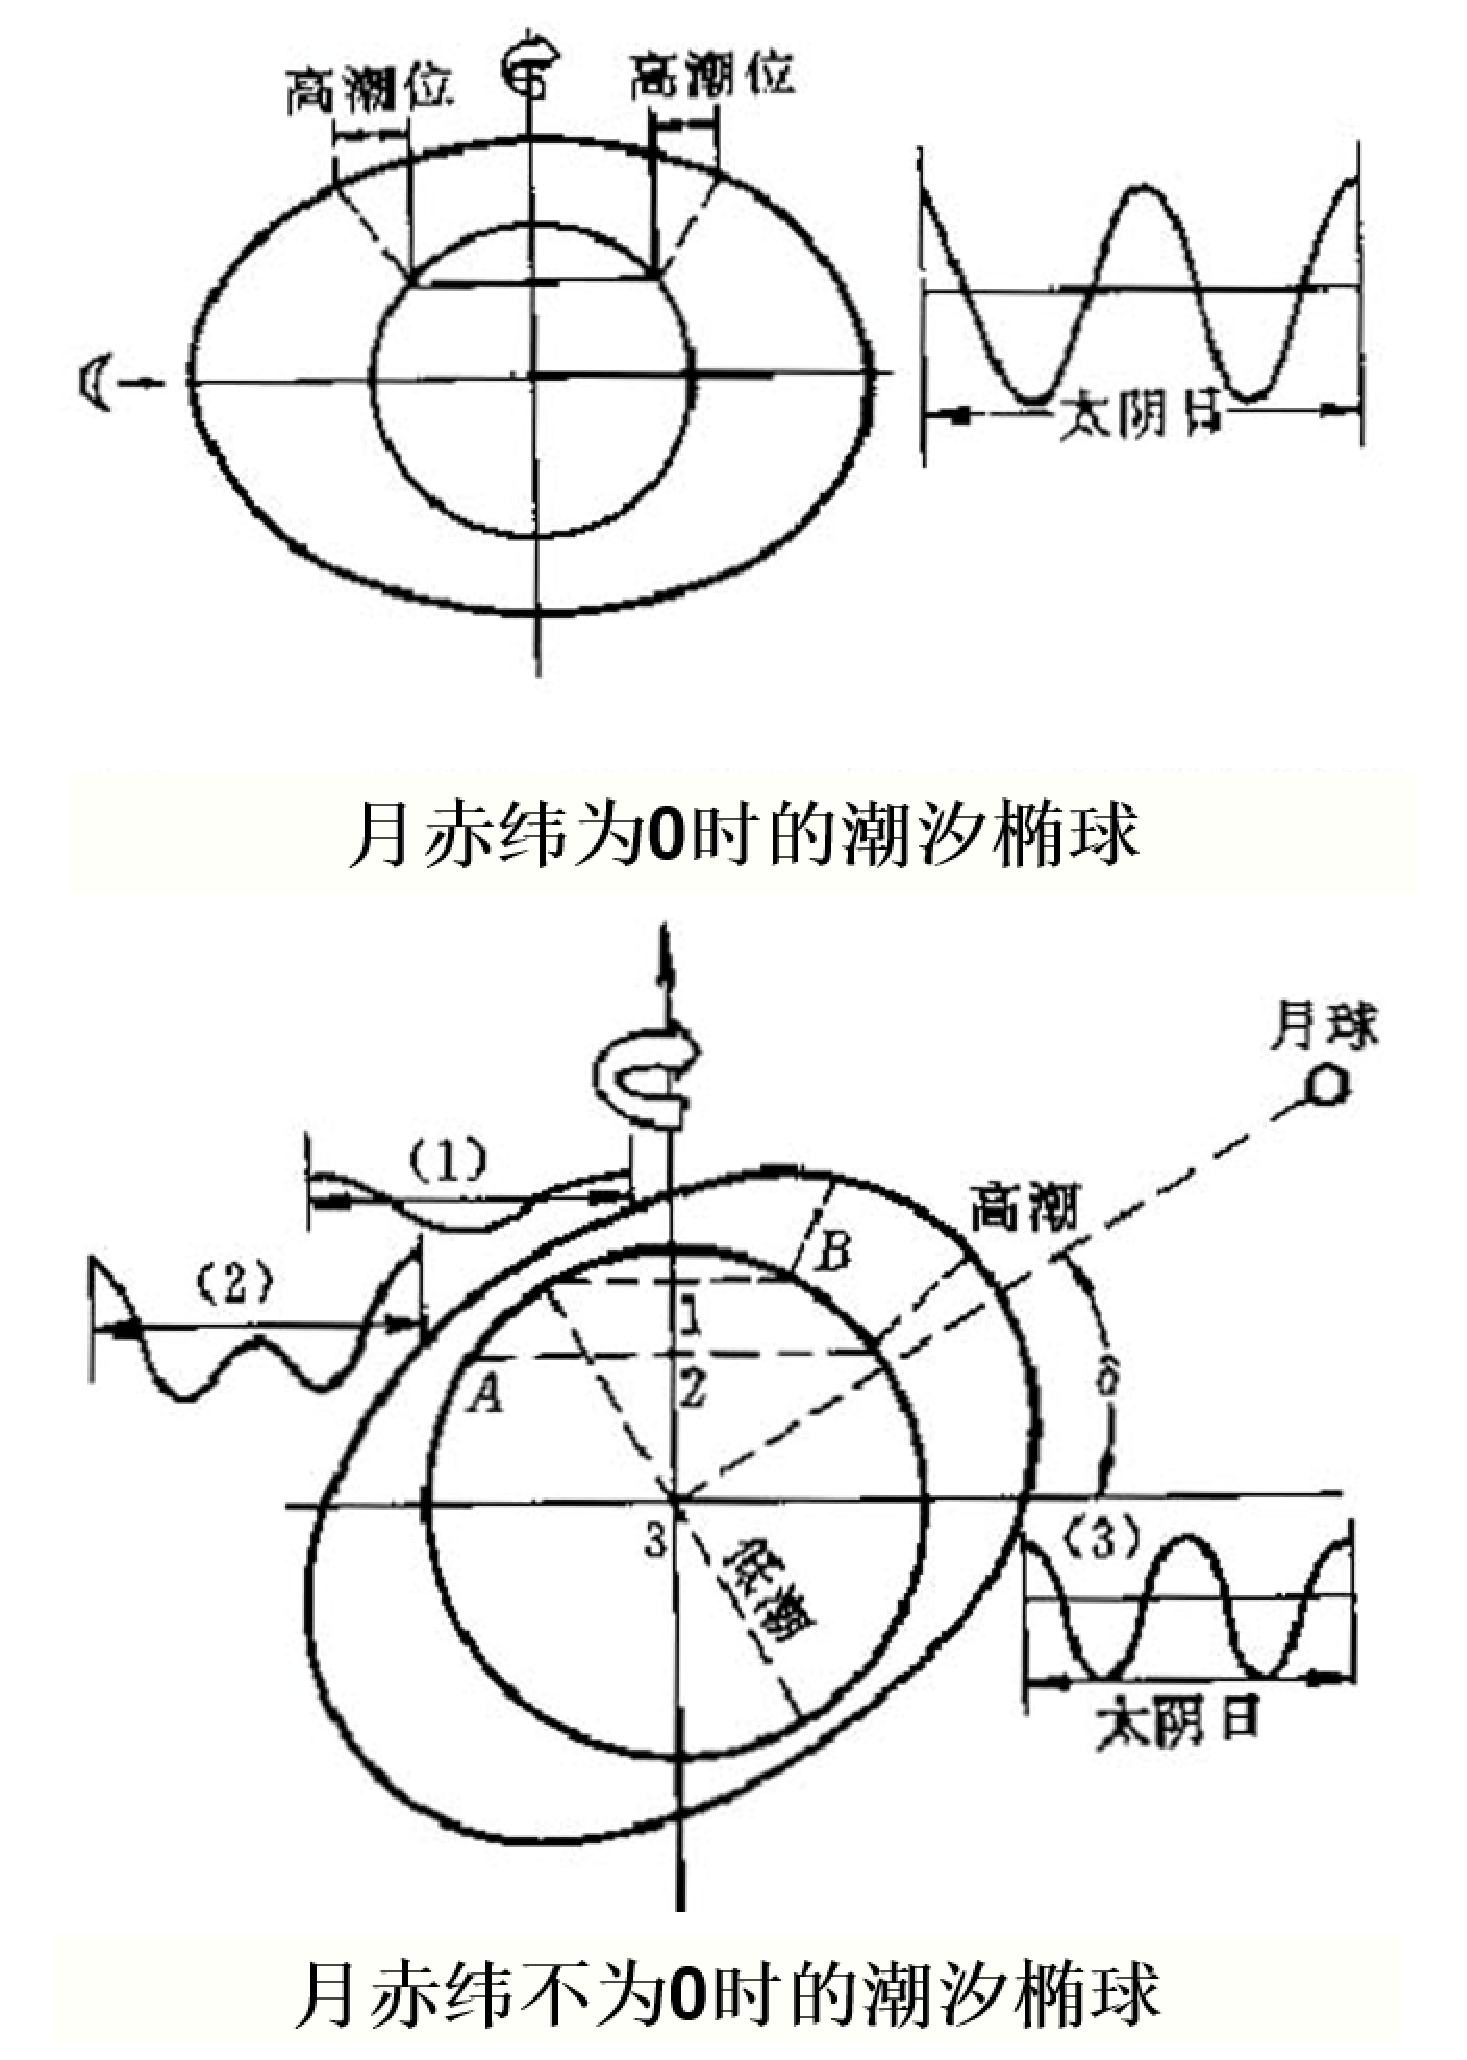
\includegraphics[width=8cm]{36.eps}
        \caption*{}
    \end{figure}
    \[
        {\bar \zeta _M} = {\bar \zeta _0} + {\bar \zeta _1} + {\bar \zeta _2} = 2G{({{\bar D} \over D})^3}\left\{ {\left[ {{3 \over 2}({{\sin }^2}\varphi  - {1 \over 3})({{\sin }^2}\delta  - {1 \over 3})} \right]} \right. + {1 \over 2}\sin 2\varphi \sin 2\delta \cos {T_1} + {1 \over 2}{\cos ^2}\varphi {\cos ^2}\delta \cos 2{T_1}\left. {} \right\}
    \]
    \paragraph{潮汐月不等}~{}\\
    由月球(太阳)引潮力引起的海水静力平衡下的海面为潮汐椭球,长轴指向月球(太阳)中心;\\
    当太阳和月球的潮汐椭球长轴重叠时,形成(朔望)大潮;长轴垂直时,形成(两弦)小潮;\\
    同时考虑月球和太阳平衡潮高可解释潮汐月不等现象.
    \begin{figure}[H]
        \centering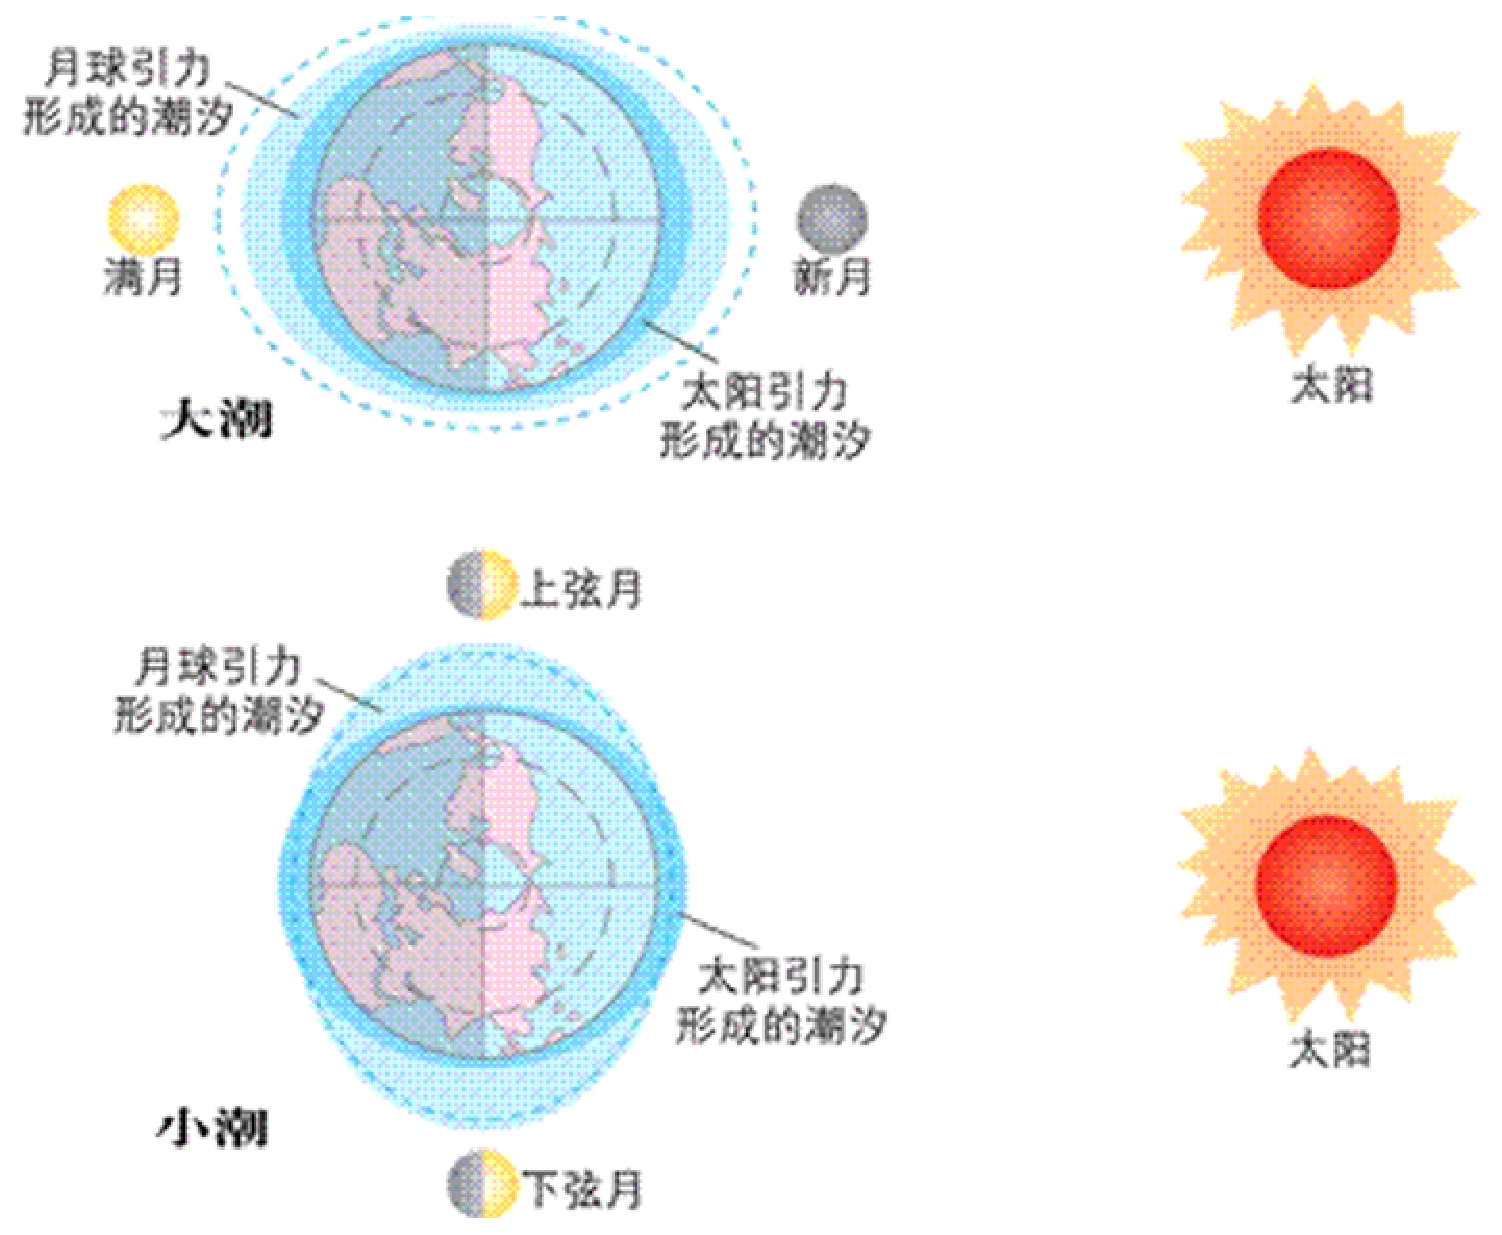
\includegraphics[width=10cm]{37.eps}
        \caption*{}
    \end{figure}
    \[
       {\bar \zeta _T} = {\bar \zeta _M}{\rm{ + }}{\bar \zeta _{\rm{S}}}
    \]
    太阴、太阳时角相差0°或180°时, 潮差最大;\\
    而当太阴、太阳时角相差90°或270°,则潮差最小
    \subsubsection{平衡潮的分潮}
    假想天体:实际海洋潮汐具有由地、月、日相对运动所产生的复杂周期。可将表示海水涨落的潮位变化曲线分解为许多不同周期的简单波动,每个单一波动对应着一个天体,即“假想天体” 。许多假想天体共同作用、将所对应的潮汐叠加,逼近实际潮潮汐。\\
    分潮:每个假想天体对海水作用引起的潮汐称为分潮。例如,$M_2$为理想的月球产生的半太阴日分潮。它的周期和月球的周期相同,位于赤道平面上,绕地球匀速公转的轨道是一个圆周,地球就在这圆的圆心。 $S_2,K_1,O_1$……\\
    \subsubsection{平衡潮理论的主要结论}
    1. 地球自转,地球表面相对椭球形海面运动,使固定点海面发生周期性的涨落;\\
    2. 月赤纬为0时,出现正规半日潮;\\
    3. 月赤纬不为0时:\\
    赤道出现正规半日潮;
    高纬地区出现正规日潮;
    其他纬度出现潮汐日不等现象;\\
    4. 每天的高潮出现在月中天;\\
    5. 同时考虑月球和太阳对潮汐的效应,形成朔望大潮;两弦小潮.
    \subsubsection{平衡潮理论的贡献}
    1. 建立在客观存在的引潮力之上,能够描述潮汐的发生;\\
    2. 计算出的最大可能潮差为78cm, 与实际大洋的潮差相近;\\
    3. 揭示的潮汐变化周期与实际基本相符;\\
    4. 能够解释潮汐日不等现象和月不等现象;\\
    5.能够解释分潮叠加,利用建立在“假想天体”和“分潮”概念上的调和分析可进行较准确的潮汐预报.
    \subsubsection{平衡潮理论的缺陷}
    1. 假定整个地球完全被等深海水包围,无法体现水深和地形对潮高的影响;\\
    2. 完全不考虑海水的运动,假设海水没有惯性和摩擦,无法体现高潮间隙和潮龄;\\
    3. 没涉及海水的水平运动,无法解释潮流这一重要现象;\\
    4. 无法解释旋转潮波系统;\\
    5. 最大潮差与浅海、近岸地区的实际况相差较大;\\
    6. 潮高振幅随纬度变化与实际不符;\\
    7. 赤道上永远不会出现日潮,低纬度地区以半日潮占优势的结论与实际不符.
    \subsection{考虑地球形状的潮波}
    \subsubsection{全球水域中的潮波(Laplace理论)}
    全球为海水覆盖,水深随纬度变化的大洋在天体引潮力的作用下产生的强迫波动.
    \paragraph{假定和方程简化}~{}\\
    对大尺度强迫潮波运动: \\
    1. 忽略惯性项中的平流项\\
    2. 忽略摩擦项\\
    3. 满足准静力近似:$\displaystyle {1 \over \rho }{{\partial p} \over {\partial \lambda }} \to g{{\partial \zeta } \over {\partial \lambda }}$\\
    4. $\rho$为常数.\\
    求坐标系下原始方程:
    \[
        {{du} \over {dt}} = 2\omega \sin \varphi v \cancel{- 2\omega \cos \varphi w }- {1 \over {\rho r\cos \varphi }}{{\partial p} \over {\partial \lambda }} - {1 \over {r\cos \varphi }}{{\partial \phi } \over {\partial \lambda }} + \cancel{{\mu  \over \rho }{(\Delta \mathord{\buildrel{\lower3pt\hbox{$\scriptscriptstyle\rightharpoonup$}}\over 
V} )_\lambda }} + \cancel{Turbulence\ Item}
    \]
    \paragraph{均质海洋垂直平均的基本方程}~{}\\
    简化运动方程:
    \[
        {{\partial u} \over {\partial t}} - 2\omega \sin \varphi v =  - {g \over {r\cos \varphi }}{{\partial \zeta } \over {\partial \lambda }} - {1 \over {r\cos \varphi }}{{\partial \phi } \over {\partial \lambda }}
    \]
    余纬度:$\theta=90^\circ-\varphi,a=r,h+\zeta\approx h$\\
    垂向平均运动方程:
    \[
        \left\{
        \begin{aligned}
            &{{\partial \left\langle u \right\rangle } \over {\partial t}} - 2\omega \cos \theta \left\langle v \right\rangle  =  - {g \over {a\sin \theta }}{{\partial \zeta } \over {\partial \lambda }} - {1 \over {a\sin \theta }}{{\partial \phi } \over {\partial \lambda }}\\
            &{{\partial \left\langle v \right\rangle } \over {\partial t}} + 2\omega \cos \theta \left\langle u \right\rangle  = {g \over a}{{\partial \zeta } \over {\partial \theta }} + {1 \over a}{{\partial \phi } \over {\partial \theta }}
        \end{aligned}
        \right.
    \]
    垂向平均连续方程:
    \[
        {{\partial \zeta } \over {\partial t}} + {{\partial \left[ {(h + \zeta )\left\langle u \right\rangle } \right]} \over {\partial x}} + {{\partial \left[ {(h + \zeta )\left\langle v \right\rangle } \right]} \over {\partial y}} = 0,{\partial  \over {\partial x}} = {1 \over {r\cos \varphi }}{\partial  \over {\partial \lambda }},{\partial  \over {\partial y}} = {1 \over r}{\partial  \over {\partial \varphi }}
    \]
    \[
        \Rightarrow {{\partial \zeta } \over {\partial t}} + {1 \over {a\sin \theta }}\left[ {{\partial  \over {\partial \theta }}( - h\left\langle v \right\rangle \sin \theta ) + {{\partial h\left\langle u \right\rangle } \over {\partial \lambda }}} \right] = 0
    \]
    球坐标潮波运动方程组:
    \[
        \left\{
            \begin{aligned}
                &{{\partial \left\langle u \right\rangle } \over {\partial t}} - 2\omega \cos \theta \left\langle v \right\rangle  =  - {g \over {a\sin \theta }}{{\partial \zeta } \over {\partial \lambda }} - {1 \over {a\sin \theta }}{{\partial \phi } \over {\partial \lambda }}\\
                &{{\partial \left\langle v \right\rangle } \over {\partial t}} + 2\omega \cos \theta \left\langle u \right\rangle  = {g \over a}{{\partial \zeta } \over {\partial \theta }} + {1 \over a}{{\partial \phi } \over {\partial \theta }}\\
                &{{\partial \zeta } \over {\partial t}} + {1 \over {a\sin \theta }}\left[ {{\partial  \over {\partial \theta }}( - h\left\langle v \right\rangle \sin \theta ) + {{\partial h\left\langle u \right\rangle } \over {\partial \lambda }}} \right] = 0
            \end{aligned}
        \right.
    \]
    根据平衡潮理论:\\
    $$displaystyle \bar{\zeta_M}=-{V_M \over g}\Rightarrow \bar{\zeta}=-{\phi \over g}$$
    \[
        {{\partial u} \over {\partial t}} - 2\omega \cos \theta v =  - {g \over {a\sin \theta }}{{\partial \zeta } \over {\partial \lambda }} - {1 \over {a\sin \theta }}{{\partial \phi } \over {\partial \lambda }}\Rightarrow {{\partial u} \over {\partial t}} - 2\omega \cos \theta v =  - {g \over {a\sin \theta }}{\partial  \over {\partial \lambda }}(\zeta  - \bar \zeta )
    \]
    \[
        {{\partial v} \over {\partial t}} + 2\omega \cos \theta u = {g \over a}{{\partial \zeta } \over {\partial \theta }} + {1 \over a}{{\partial \phi } \over {\partial \theta }}\Rightarrow {{\partial v} \over {\partial t}} + 2\omega \cos \theta u = {g \over a}{\partial  \over {\partial \theta }}(\zeta  - \bar \zeta )
    \]
    平衡潮潮高公式:
    \[
        \begin{aligned}
            {{\bar \zeta }_M} &= {{\bar \zeta }_0} + {{\bar \zeta }_1} + {{\bar \zeta }_2}\\
            &= 2G{\left( {{{\bar D} \over D}} \right)^3}\left\{\left[ {3 \over 2}({{\sin }^2}\varphi  - {1 \over 3})({{\sin }^2}\delta  - {1 \over 3}) \right]  +{1 \over 2}\sin 2\varphi \sin 2\delta \cos {T_1} + {1 \over 2}{\cos ^2}\varphi {\cos ^2}\delta \cos 2T_1\right\}
        \end{aligned}
    \]
    令:$\displaystyle {H_0} = 3G{({{\bar D} \over D})^3}({1 \over 3} - {\sin ^2}\delta ),{H_1} = 2G{({{\bar D} \over D})^3}\sin 2\delta ,{H_2} = G{({{\bar D} \over D})^3}{\cos ^2}\delta $
    将纬度以余纬度替换:
    \[
        \bar \zeta  = {H_0}({1 \over 3} - {\cos ^2}\theta ) + {H_1}\sin \theta \cos \theta \cos {T_1} + {H_2}{\sin ^2}\theta \cos 2{T_1}
    \]
    \begin{figure}[H]
        \centering 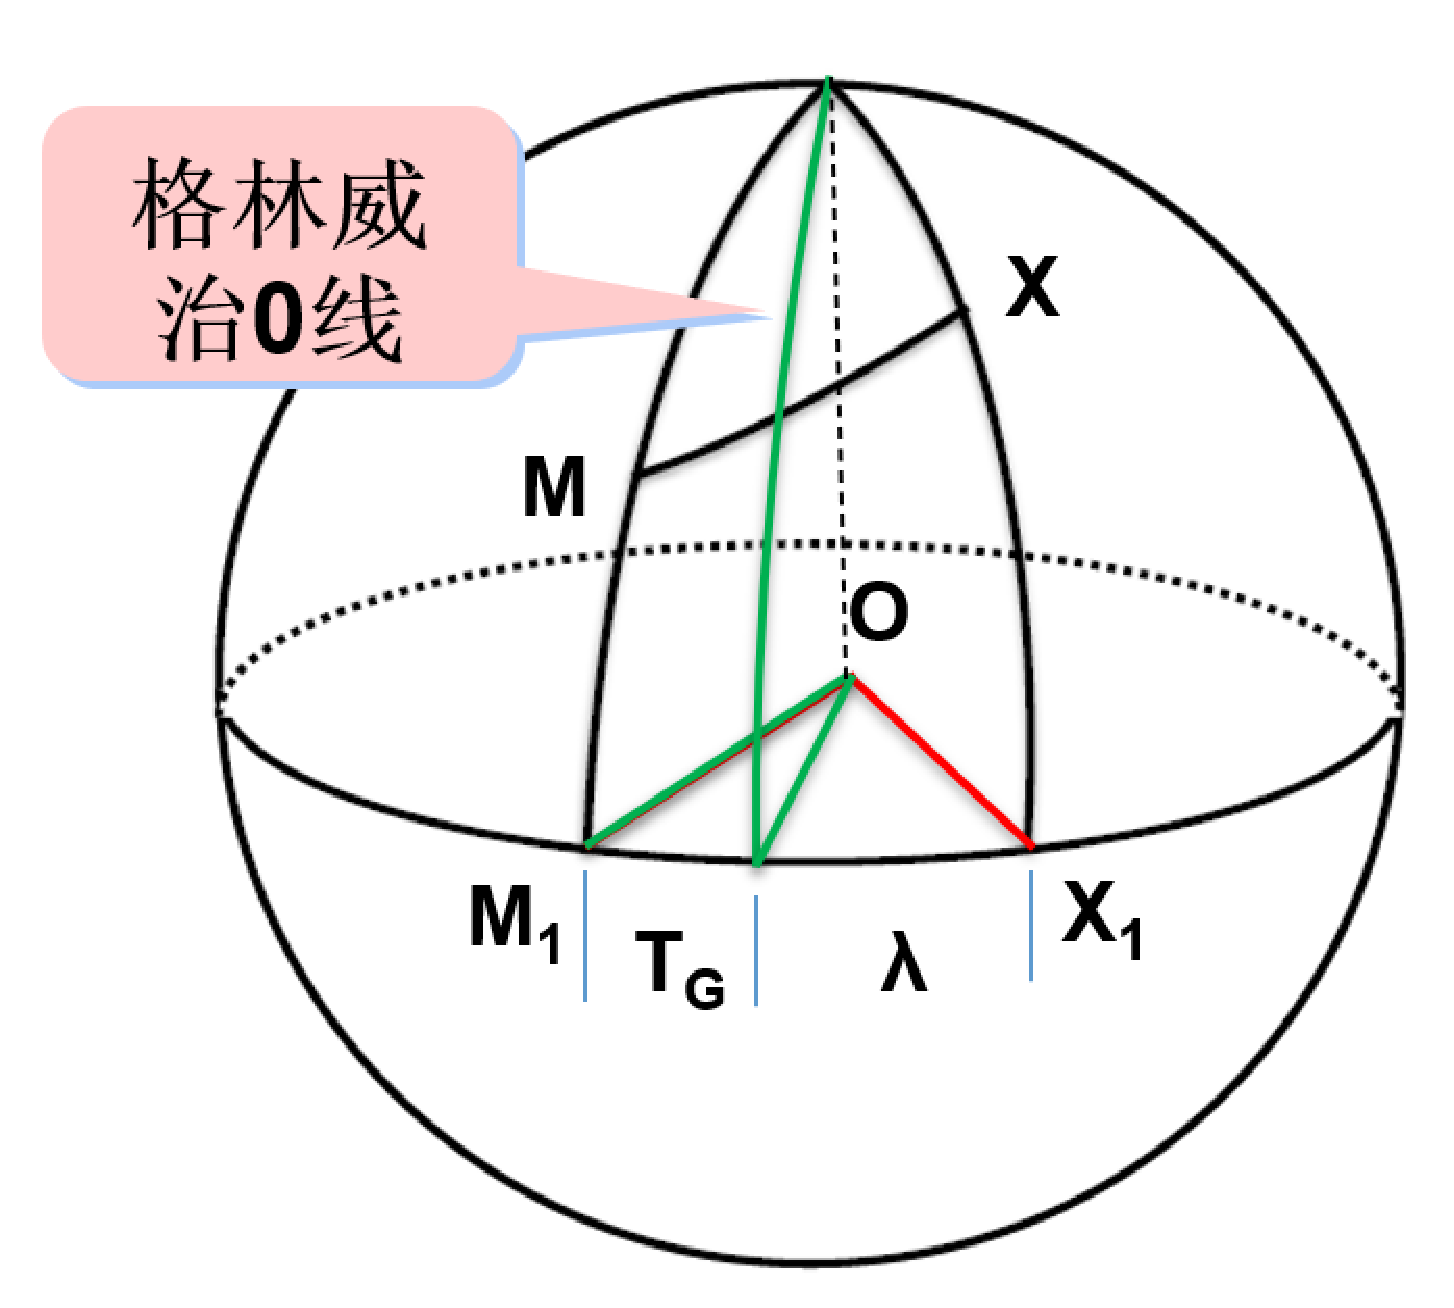
\includegraphics[width=10cm]{38.eps}
        \caption*{}
    \end{figure}
    \[
        T_1=T_G+\lambda=\omega_1 t+180^\circ +\lambda
    \]
    $T_1$为观测点的月球时角,$T_G$为格林威治的月球时角,$\lambda$为经度(东经取正号),$t$为格林威治平太阴时,${\omega _1} = {360^ \circ }/24 = {15^ \circ }/$平太阴时.\\
    月球平衡潮的三类潮高:
    \[
        \begin{aligned}
            &{\bar \zeta _0} = {H_0}({1 \over 3} - {\cos ^2}\theta )\\
            &{\bar \zeta _1} = {H_1}\sin \theta \cos \theta \cos ({\omega _1}t{\rm{ + }}\lambda  + {180^ \circ })\\
            &{\bar \zeta _2} = {H_2}{\sin ^2}\theta \cos ({\omega _2}t{\rm{ + }}2\lambda  + 2 \times {180^ \circ })
        \end{aligned}
    \]
    其中,${\omega _2} = 2{\omega _1}$.
    各类潮波:
    \[
        {\zeta _n},{\bar \zeta _n},{u_n},{v_n} \to {e^{i({\omega _n}t + n\lambda  + {\alpha _n})}}{\rm{  }}(n = 0,1,2)
    \]
    带入运动方程和连续方程:
    \[
        {\zeta '_n} = {\zeta _n} - {\bar \zeta _n};  {\bar \omega _n} = {\omega _n}/(2\omega );  {m_n} = 4\omega _n^2a/g  (n = 0,1,2)
    \]
    Laplace潮汐方程:
    \[
        {1 \over {\sin \theta }}{d \over {d\theta }}[{{h\sin \theta } \over {{{\bar \omega }_n} - {{\cos }^2}\theta }}({{d{{\zeta '}_n}} \over {d\theta }} + {n \over {{{\bar \omega }_n}}}{\zeta '_n}\cot \theta )] - {h \over {{{\bar \omega }_n} - {{\cos }^2}\theta }} \times ({n \over {{{\bar \omega }_n}}}\cot \theta {{d{{\zeta '}_n}} \over {d\theta }} + {n^2}{\zeta '_n}\cos ec\theta ) + {m_n}a{\zeta '_n} =  - {m_n}a{\bar \zeta _n}
    \]
    \paragraph{讨论}~{}\\
    1. 长周期潮($n$=0)\\
    令$\mu=\cos\theta,\theta=90^\circ-\varphi,h=2210m$:
    \[
        {\zeta _0} = {\zeta '_0} + {\bar \zeta _0} = {H_0}(0.1515 - 1.0{\mu ^2} + 1.5153{\mu ^4} - .... + ...
    \]
    比较动力潮和平衡潮在赤道和极低的潮高:\\
    两极:$\displaystyle {\zeta _0}\mu  =  \pm 1 =  - {2 \over 3}{H_0} \cdot 0.154,\bar{\zeta}_0=-{2 \over 3}H_0$\\
    赤道:$\displaystyle {\zeta _0}\mu  = 0 = {1 \over 3}{H_0} \cdot 0.455,\bar{\zeta}_0={1 \over 3}H_0$\\
    长周期的动力潮高小于长周期的平衡潮高.\\
    2. 全日潮($n=1$)\\
    3. 半日潮($n=2$)
    \subsubsection{有界水域中的潮波(Airy沟渠理论)}~{}
    \subsection{等深广阔水域中的潮波}
    \[
        \boxed{\mbox{相同的动力学方程}}+\boxed{\mbox{不同的边界条件}}\Rightarrow \boxed{\mbox{不同的频散关系}}\Rightarrow \boxed{\mbox{不同性质的波动}}
    \]
    \paragraph{假定和方程}~{}\\
    1. 宽广平缓的陆家海:(1) 等深 (2) 大尺度(忽略非线性平流项;忽略摩擦)\\
    2. 自由波动\\
    3. 均质,密度为常数\\
    4. 静力近似\\
    5. $f$平面近似\\
    垂向平均方程组:
    \begin{numcases}{}
        \frac{\partial u}{\partial t}-f v=-g \frac{\partial \zeta}{\partial x} \label{tide1}\\
        \frac{\partial v}{\partial t}+f u=-g \frac{\partial \zeta}{\partial y}\label{tide2}\\
        \frac{\partial \zeta}{\partial t}+h\left(\frac{\partial u}{\partial x}+\frac{\partial v}{\partial y}\right)=0\label{tide3}
    \end{numcases}
    其中假设$h+\zeta\approx h$.\\
    设波动解:
    \[
        \left\{
            \begin{aligned}
                &\zeta=Z(x,y)e^{-i\omega t}\\
                &u=U(x,y)e^{-i\omega t}\\
                &v=V(x,y)e^{-i\omega t}
            \end{aligned}
        \right.
    \]
    带入(\ref{tide1}),(\ref{tide2},得极化方程:
    \[
        \left\{\begin{aligned}
            &-i \omega U-f V=-g \frac{\partial Z}{\partial x} \\
            &-i \omega V+f U=-g \frac{\partial Z}{\partial y}
            \end{aligned} \Rightarrow\left\{\begin{aligned}
            &U=\frac{g}{\omega^{2}-f^{2}}\left(-i \omega \frac{\partial Z}{\partial x}+f \frac{\partial Z}{\partial y}\right) \\
            &V=\frac{g}{\omega^{2}-f^{2}}\left(-i \omega \frac{\partial Z}{\partial y}-f \frac{\partial Z}{\partial x}\right)
            \end{aligned}\right.\right.
    \]
    带入(\ref{tide3}),$f$为常数,得Helmholtz方程:
    \[
        \frac{\partial^{2} Z}{\partial x^{2}}+\frac{\partial^{2} Z}{\partial y^{2}}+\frac{\omega^{2}-f^{2}}{g h} Z=0
    \]
    用分离变量法令$Z(x,y)=X(x)Y(y)$:
    \[
        \frac{X^{\prime \prime}}{X}+\frac{Y^{\prime \prime}}{Y}+\frac{\omega^{2}-f^{2}}{g h}=0 \Rightarrow \frac{X^{\prime \prime}}{X}+\frac{\omega^{2}-f^{2}}{g h}=-\frac{Y^{\prime \prime}}{Y}=c o n s t
    \]
    其中,$\displaystyle const=\left\{\begin{aligned}  &l^{2} (\mbox{平面Sverdrup波})\\  &0 \\ &-l^{2}\mbox{Kelvin波}\end{aligned}\right.$
    \subsubsection{平面Sverdrup波}
    \[
        \omega^2=f^2+(k^2+l^2)gh
    \]
    \[
        \left\{
            \begin{aligned}
                &X^{\prime \prime}+k^{2} X=0\\
                &Y^{\prime \prime}+l^{2} Y=0
            \end{aligned}
        \right.
        \Rightarrow\left\{\begin{aligned}
            &X=A_{1} e^{-i k x}+B_{1} e^{i k x} \\
            &Y=A_{2} e^{-i l y}+B_{2} e^{i l y}
            \end{aligned}\right.
    \]
    带入$Z(x,y)=X(x)Y(y)$:
    \[
        \begin{array}{l}
            Z=c_{1} e^{i(k x+l y)}+c_{2} e^{i(k x-l y)}+c_{3} e^{-i(k x+l y)}+c_{4} e^{-i(k x-l y)} \\
            c_{1}=B_{1} B_{2} ; \quad c_{2}=B_{1} A_{2} ; \quad c_{3}=A_{1} A_{2} ; \quad c_{4}=A_{1} B_{2}
            \end{array}
    \]
    四个沿不同方向传播的同一性质的波动的叠加.
    取其中的$Z=Ae^{i(kx+ly)}$带入极化方程:
    \[
        \left\{\begin{aligned}            U=\frac{g}{\omega^{2}-f^{2}}\left(-i \omega \frac{\partial Z}{\partial x}+f \frac{\partial Z}{\partial y}\right) \\
            V=\frac{g}{\omega^{2}-f^{2}}\left(-i \omega \frac{\partial Z}{\partial y}-f \frac{\partial Z}{\partial x}\right)
            \end{aligned} \quad \Rightarrow \left\{\begin{aligned}
            U=\frac{A g}{\omega^{2}-f^{2}}(\omega k+i f l) e^{i(k x+l y)} \\
            V=\frac{A g}{\omega^{2}-f^{2}}(\omega l-i f k) e^{i(k x+l y)}
            \end{aligned}\right.\right.
    \]
    结合频散关系:
    \[
        \left\{\begin{aligned}
            \zeta=A e^{i(k x+l y-\omega t)} \\
            u=A_{u} e^{i(k x+l y-\omega t)} \\
            v=A_{v} e^{i(k x+l y-\omega t)}
            \end{aligned}\right.
    \]
    其中,$\displaystyle  A_{u}=\frac{A}{h} \frac{\omega k+i f l}{k^{2}+l^{2}},  A_{v}=\frac{A}{h} \frac{\omega l-i f k}{k^{2}+l^{2}}$\\
    \paragraph{Sverdrup波存在条件}~{}
    \[
        k^{2}=\frac{\omega^{2}-f^{2}}{g h}-l^{2} \Rightarrow k^{2}+l^{2}=\frac{\omega^{2}-f^{2}}{g h}
    \]
    因此Sverdrup波存在的条件为$\omega^2>f^2$.\\
    \paragraph{频散关系}~{}\\
    将$x$轴取在波动传播方向:$\omega^2=f^2+ghm^2,m^2=k^2+l^2$\\
    浅水重力波:$\omega^2=gdk^2$\\
    Sverdrup波的频率的平方为科氏参数和浅水波频率的平方和.
    \paragraph{波速和群速}~{}\\
    波速:$\displaystyle c=\frac{\lambda}{T}=\frac{\omega}{m}=\sqrt{\frac{\omega^{2}}{m^{2}}}=\sqrt{g h} \sqrt{\frac{1}{1-\left(\frac{f}{\omega}\right)^{2}}}>\sqrt{g h}$\\
    Sverdrup波的波速大于浅水波波速.
    群速:$\displaystyle c_{g}=\frac{d \omega}{d m}=\frac{1}{2}\left(\omega^{2}\right)^{-\frac{1}{2}} \cdot(2 m g h)=\sqrt{g h} \sqrt{1-\left(\frac{f}{\omega}\right)^{2}}<\sqrt{g h}$\\
    Sverdrup波的群速小于浅水波波速.
    \paragraph{流速和流向}~{}\\
    \[
        \left\{\begin{aligned}
            \zeta=A e^{i(k x+l y-\omega t)} \\
            u=A_{u} e^{i(k x+l y-\omega t)} \\
            v=A_{v} e^{i(k x+l y-\omega t)}
            \end{aligned} \right. \Rightarrow
    \]
    \begin{numcases}{}
        \zeta=A \cos (k x-\omega t) \nonumber \\
        u=\frac{\omega}{k h} A \cos (k x-\omega t) \label{x1}\\
        v=\frac{f}{k h} A \sin (k x-\omega t) \label{x2}
    \end{numcases}
    由(\ref{x1}),(\ref{x2})得:
    \[
        \frac{u^{2}}{\left(\frac{\omega A}{k h}\right)^{2}}+\frac{v^{2}}{\left(\frac{f A}{k h}\right)^{2}}=1
    \]
    流速矢端的轨迹为一椭圆 ,长轴沿波动传播方向.\\
    流失量与$x$轴的夹角:$\displaystyle \theta=\arctan {v\over u}$\\
    \[
        \frac{d \theta}{d t}=\frac{1}{1+\left(\frac{v}{u}\right)^{2}} \cdot \frac{d}{d t}\left(\frac{v}{u}\right)=\frac{-\omega^{2} A^{2} f}{k^{2} h^{2}\left(u^{2}+v^{2}\right)}
    \]
    前进潮波中的旋转潮流是由于地转偏向力作用的结果,在北半球,流矢量随时间作顺时针旋转.\\
    Sverdrup波的平均动能大于平均势能,平均能量只沿波动传播方向转移.
    \[
        \bar{p}=\frac{1}{2} \rho g a^{2} \cdot c
    \]
    \paragraph{地转效应引起的变化(与浅水重力波相比)}~{}\\
    1. Sverdrup波的频率比浅水波的频率大。其平方等于浅水波频率与科氏参数的平方和;\\
    2. Sverdrup波的波速大于浅水波波速,群速小于浅水波波速;\\
    3. Sverdrup波的垂直波动传播方向的速度(横向速度)$v$不再等于0,产生旋转潮流;\\
    4. Sverdrup波的平均动能大于平均势能.
    \subsubsection{Poincare波}
    Sverdrup波遇到直线海岸将发生反射,入射波和反射波叠加形成Poincare波.\\
    1. 沿x正方向传播的前进波,岸界在传播方向的右方,称右界Poincare波;\\
    2. 沿x负方向传播的前进波,岸界在传播方向的左方,称左界Poincare波;\\
    3. 等振幅线平行岸线,振幅沿y方向呈余弦变化;\\
    4. 入射波与岸界垂直时,产生驻立Sverdrup波.
    \subsubsection{Kelvin波}
	\paragraph{频散关系和波动解}~{}
	频散关系:
	$$\omega^2=ghk^2$$
	\indent
	波动解:
	\[
	\left\{
	\begin{aligned}
		\zeta & = A{e^{ - {f \over c}y}} \cdot {e^{i(kx - \omega t)}}\\
		u &= {g \over c}A{e^{ - {f \over c}y}} \cdot {e^{i(kx - \omega t)}}\\
		v&=0
	\end{aligned}	
	\right.
	\]
	\indent
	上面的解未考虑底摩擦,若考虑,则波动解为:
	\[
	\left\{
	\begin{aligned}
		&\zeta=A e^{-\left(\alpha_{1} y+\beta_{1} x\right)} \cos \left(\alpha_{2} y+\beta_{2} x-\omega t\right)\\
		&u=\frac{g}{\sqrt{g h}} \frac{1}{\sqrt[4]{1+\mu^{2}}} A e^{-\left(\alpha_{1} y+\beta_{1} x\right)} \cos \left(\alpha_{2} y+\beta_{2} x-\omega t-r\right)\\
		&v=0
	\end{aligned}
	\right.
	\]
	其中,
	\[
	\left\{
	\begin{aligned}
	&\alpha_{1}=\frac{f}{\sqrt{g h}} \sqrt{\frac{\sqrt{1+\mu^{2}}+1}{2\left(1+\mu^{2}\right)}}\\
	&\beta_{1}=\frac{\omega}{\sqrt{g h}} \sqrt{\frac{\sqrt{1+\mu^{2}}-1}{2}}\\
	&\alpha_{2}=\frac{f}{\sqrt{g h}} \sqrt{\frac{\sqrt{1+\mu^{2}}-1}{2\left(1+\mu^{2}\right)}}\\
	&\beta_{2}=\frac{\omega}{\sqrt{g h}} \sqrt{\frac{\sqrt{1+\mu^{2}}+1}{2}}\\
	&\mu=k/\omega\\
	&r=\arctan \sqrt{\frac{\sqrt{1+\mu^{2}}-1}{\sqrt{1+\mu^{2}}+1}}
	\end{aligned}
	\right.
	\]
	\newpage
	\paragraph{两列传播方向相反的Kelvin波叠加}
	\begin{figure}[H]
		\centering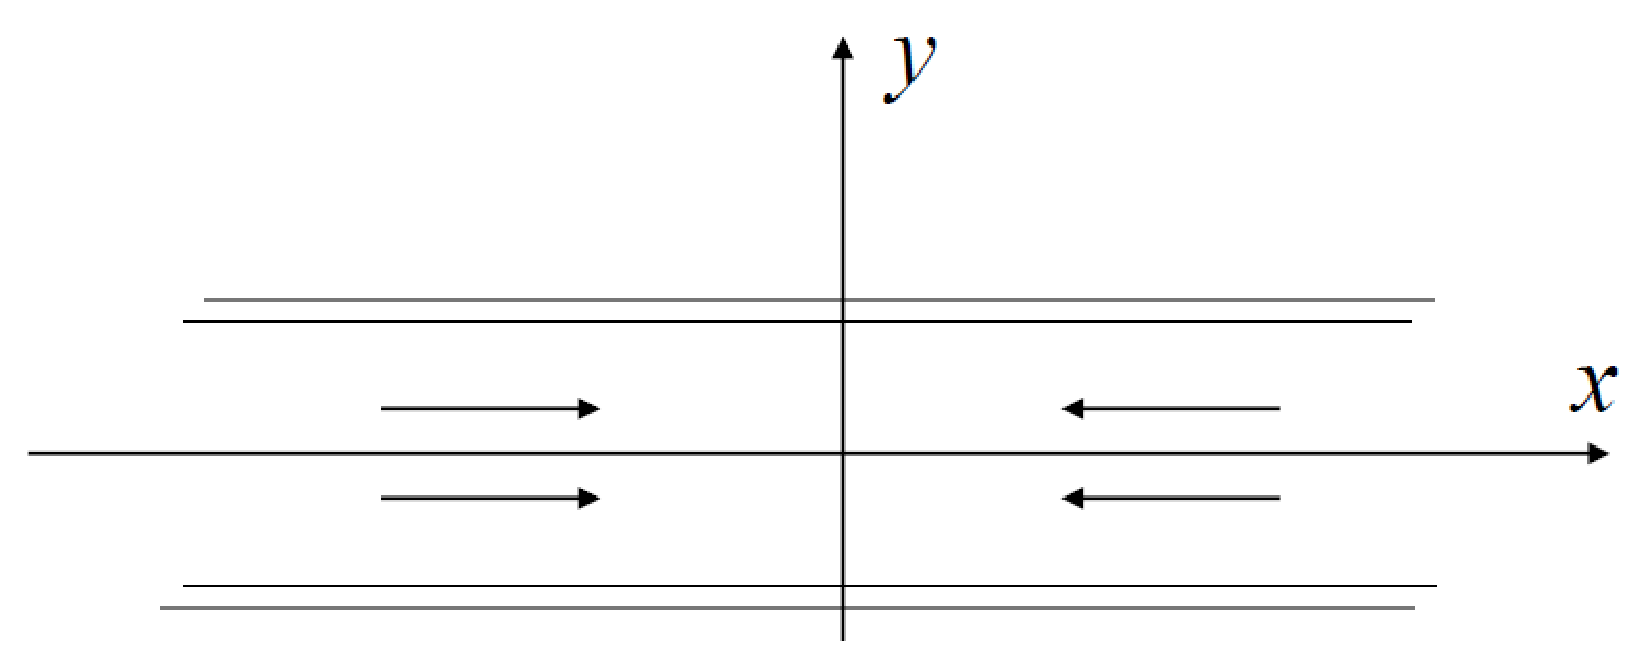
\includegraphics[width=10cm]{39.eps}
		\caption*{}
	\end{figure}
	在波向平行海峡,海峡无限长、深且等深、较宽的条件下,两列性质相同但传播方向相反的Kelvin波叠加后的水位可以表示为:
	\[
	\zeta=Ae^{-\frac{f}{c}y}e^{i(kx-\omega t)}+Ae^{\frac{f}{c}y}e^{i(-kx-\omega t)}
	\]
	\indent
	取实部:
	\[
	\zeta=2 A {\rm ch}\left(\frac{f}{c} y\right) \cos \frac{\omega}{c} x\cos\omega t-2 A {\rm sh}\left(\frac{f}{c}y\right) \sin\frac{\omega}{c}x\sin\omega t
	\]
	\indent
	令:
	\[
	\zeta_1=2 A {\rm ch}\left(\frac{f}{c} y\right) \cos \frac{\omega}{c} x=R\cos\theta,
	\zeta_2=-2 A {\rm sh}\left(\frac{f}{c}y\right) \sin\frac{\omega}{c} x=R\sin\theta
	\]
	其中,$R=\sqrt{\zeta_1^2+\zeta_2^2},\theta=\arctan\frac{\zeta_1}{\zeta_2}$
	,因此:
	\[
	\zeta=R\cos(\omega t-\theta)
	\]
	\indent
	性质:\\
	\indent
	\textbf {1) 无潮点}
	\[
	\begin{aligned}
	R=0&\Rightarrow {\rm ch}^{2} \frac{f}{c} y \cos ^{2} \frac{\omega}{c} x+{\rm sh}^{2} \frac{f}{c} y \sin ^{2} \frac{\omega}{c} x=0\\
	&\Rightarrow {\rm ch}^{2} \frac{f}{c} y - {\rm ch}^{2} \frac{f}{c} y\sin ^{2} \frac{\omega}{c} x+{\rm sh}^{2} \frac{f}{c} y \sin ^{2} \frac{\omega}{c} x=0\\
	&\Rightarrow {\rm ch}^{2} \frac{f}{c} y-\sin ^{2} \frac{\omega}{c} x=0\\
	&\Rightarrow\left\{\begin{array}{l}\frac{f}{c} y_{0}=0 \\ \frac{\omega}{c} x_{0}=\frac{2 n-1}{2} \pi \quad(n=0,\pm 1,\pm 2)\end{array}\right.\\
	&\Rightarrow\boxed{\left\{\begin{array}{l}y_{0}=0 \\ x_{0}=\frac{2 n-1}{2}  \frac{\lambda}{2}\end{array}\right.}
	\end{aligned}
	\]
	\indent
	即,无潮点位于海峡中轴线上,相邻两个无潮点之间的距离为半波长。\\
	\indent
	\textbf {2) 等振幅线}
	\[
	\begin{aligned}
	    R=const&\Rightarrow {\rm ch}^{2} \frac{f}{c} y \cos ^{2} \frac{\omega}{c} x+{\rm sh}^{2} \frac{f}{c} y \sin ^{2} \frac{\omega}{c} x=c o n s t\\
	    &\Rightarrow {\rm ch}^{2} \frac{f}{c} y-\sin ^{2} \frac{\omega}{c} x=const
	\end{aligned}
	\]
	\indent
	特别地,对于无潮点附近的等振幅线,将坐标原点移到无潮点上:
	\[
	\left\{
	\begin{aligned}
	\frac{f}{c}y&=\frac{f}{c}y^{\prime} \\
	\frac{\omega}{c}x&=\frac{\omega}{c}x^{\prime}+\frac{\pi}{2}
	\end{aligned}
	\right.
	\]
	\[
	\Rightarrow{\rm ch}^{2} \frac{f}{c} y^{\prime}-\cos ^{2} \frac{\omega}{c} x^{\prime}=const
	\]
	\[
	x^{\prime}\rightarrow 0, \cos ^{2} \frac{\omega}{c} x^{\prime}\rightarrow 1-\left( \frac{\omega}{c}x^{\prime}\right)^2;y^{\prime}\rightarrow 0, {\rm ch} ^{2} \frac{f}{c} y^{\prime}\rightarrow 1+\left( \frac{f}{c}y^{\prime}\right)^2
	\]
	\[
	\Rightarrow \boxed{\frac{x^{\prime 2}}{\left(\frac{f}{c}\right)^{2}}+\frac{y^{\prime 2}}{\left(\frac{\omega}{c}\right)^{2}}=\mathrm{const}}
	\]
	\indent
    上式表明,无潮点附近的等振幅线为椭圆族,当$\omega<f$时,长轴位于$x$轴,即平行于海峡;当$\omega>f$时,长轴位于$y$轴,即垂直于海峡。\\
    \indent
    \textbf {3) 同潮时线}\\
    \indent
    设$t_c$为发生高潮的时刻,则同潮时线由$\omega t_c-\theta=0,t_c=const$确定:
    \[
    t_c=\frac{\theta}{\omega}=\frac{1}{\omega} \arctan \frac{\zeta_{2}}{\zeta_{1}}=\frac{1}{\omega} \arctan \frac{-2  \operatorname{Ash} \frac{f}{c} y \sin \frac{\omega}{c} x}{2 \operatorname{Ach} \frac{f}{c} y \cos \frac{\omega}{c} x}=\frac{1}{\omega} \arctan \left(-\operatorname{th} \frac{f}{c} y \cdot \tan \frac{\omega}{c} x\right)=const
    \]
    \indent
    将坐标原点移到无潮点上:
    \[
    \left\{
    \begin{aligned}
    \frac{f}{c}y&=\frac{f}{c}y^{\prime} \\
    \frac{\omega}{c}x&=\frac{\omega}{c}x^{\prime}+\frac{\pi}{2}     \end{aligned}
    \right.
    \]
    \[
    \Rightarrow t_{c}=\frac{1}{\omega} \arctan \left[-t h \frac{f}{c} y^{\prime} \tan \left(\frac{\omega}{c} x^{\prime}+\frac{\pi}{2}\right)\right]=\frac{1}{\omega} \arctan \left[-t h \frac{f}{c} y^{\prime} / \tan \frac{\omega}{c} x^{\prime}\right]=const
    \]
    \indent
    利用级数展开,取第一项近似:
    \[
     \tan x=x+\frac{1}{3} x^{3}+\frac{2}{15} x^{5}+\cdots \quad {\rm th} x=x-\frac{1}{3} x^{3}+\frac{2}{15} x^{5}-\cdots
    \]
	\[
	\begin{aligned}
	&\Rightarrow t_c=\frac{1}{\omega} \arctan \left( \frac{f}{c} y^{\prime} / \frac{\omega}{c} x^{\prime} \right) \\
	&\Rightarrow \frac{f}{c} y^{\prime} / \frac{\omega}{c} x^{\prime}=\tan (\omega t_c)\\
	&\Rightarrow \boxed{y^{\prime}=\left[\frac{\omega}{f} \tan \left(\omega t_{c}\right)\right] x^{\prime}}
	\end{aligned}
	\]
	\indent
	上式表明,无潮点附近的同潮时线是直线,斜率随高潮发生时刻变化。在北半球,同潮时线绕无潮点逆时针旋转。
	\par
	综上所述,相反Kelvin波叠加在海峡中的波动特点有以下五点:
	\par
	1) 无潮点位于海峡中轴线上;
	\par
	2) 相邻两个无潮点之间的距离为半波长;
	\par
	3) 无潮点附近的等振幅线为椭圆族;,当$\omega<f$时,长轴位于$x$轴,即平行于海峡,当
	\par
	\indent
	\indent
	$\omega>f$时,长轴位于$y$轴,即垂直于海峡;
	\par
	4) 无潮点附近的同潮时线是直线,在北半球,同潮时线绕无潮点逆时针旋转;
	\par
	5) 在离开无潮点较远的地方,等振幅线不再是椭圆,同潮时线也不再是直线。
	\par
	若考虑摩擦,
	\[
		\begin{aligned} 
		\zeta=& A e^{-\left(\alpha_{1} y+\beta_{1} x\right)} \cos \left(\alpha_{2} y+\beta_{2} x-\omega t\right)+A e^{\left(\alpha_{1} y+\beta_{1} x\right)} \cos \left(\alpha_{2} y+\beta_{2} x+\omega t\right) \\
		=& 2 A\left[\operatorname{ch}\left(\alpha_{1} y+\beta_{1} x\right) \cos \left(\alpha_{2} y+\beta_{2} x\right) \cos \omega t\right.\left.-\operatorname{sh}\left(\alpha_{1} y+\beta_{1} x\right) \sin \left(\alpha_{2} y+\beta_{2} x\right) \sin \omega t\right] \\
		=&\zeta_1\cos\omega t+\zeta_2\sin\omega t 
		\end{aligned}
	\]
	其中,
	\[
	\left\{
	\begin{aligned}
	\zeta_{1}=2 \operatorname{Ach} \theta_{1} \cos \theta_{2},& \zeta_{2}=-2 \operatorname{Ash} \theta_{1} \sin \theta_{2}\\
	\theta_{1}=\alpha_{1} y+\beta_{1} x,& \theta_{2}=\alpha_{2} y+\beta_{2} x
	\end{aligned}
	\right.	
	\]
	\par
	无潮点的位置满足:
	\[
	\left\{\begin{array}{l}\theta_{1}=\alpha_{1} y_{0}+\beta_{1} x_{0}=0 \\ \theta_{2}=\alpha_{2} y_{0}+\beta_{2} x_{0}=\frac{(2 n-1)}{2} \pi, n=0,\pm 1,\pm 2, \ldots\end{array}\right.
	\]
	\[
	\Rightarrow	\left\{\begin{array}{l}x_{0}=\frac{2 n-1}{2} \pi \frac{\sqrt{g h}}{\omega} \sqrt{\frac{\sqrt{1+\mu^{2}}+1}{2}} \\ y_{0}=-\frac{2 n-1}{2} \pi \frac{\sqrt{g h}}{f} \sqrt{\frac{\sqrt{1+\mu^{2}}-1}{2}}\sqrt{1+\mu^2}\end{array}\right.
	\]
	\par
	1) $\mu=0$时,与无摩擦情况相同;
	\par
	2) $\mu\neq 0$时,$y_0\neq 0$,说明无潮点不在海峡中线上,而是向强度较强的Kelvin波的传播方向的左方偏移:
	\[
	\left\{\begin{aligned}
		&n>0,x_0>0,y_0<0\\
		&n<0,x_0<0,y_0>0
	\end{aligned}\right.
	\]
	\par
	$x$方向无潮点的间距大于半波长:
	\[
	\Delta x_{0}=\pi \frac{\sqrt{g h}}{\omega} \sqrt{\frac{\sqrt{1+\mu^{2}}+1}{2}}>\pi \frac{\sqrt{g h}}{\omega}=\frac{c T}{2}=\frac{\lambda}{2}
    \]
    \begin{figure}[H]
        \centering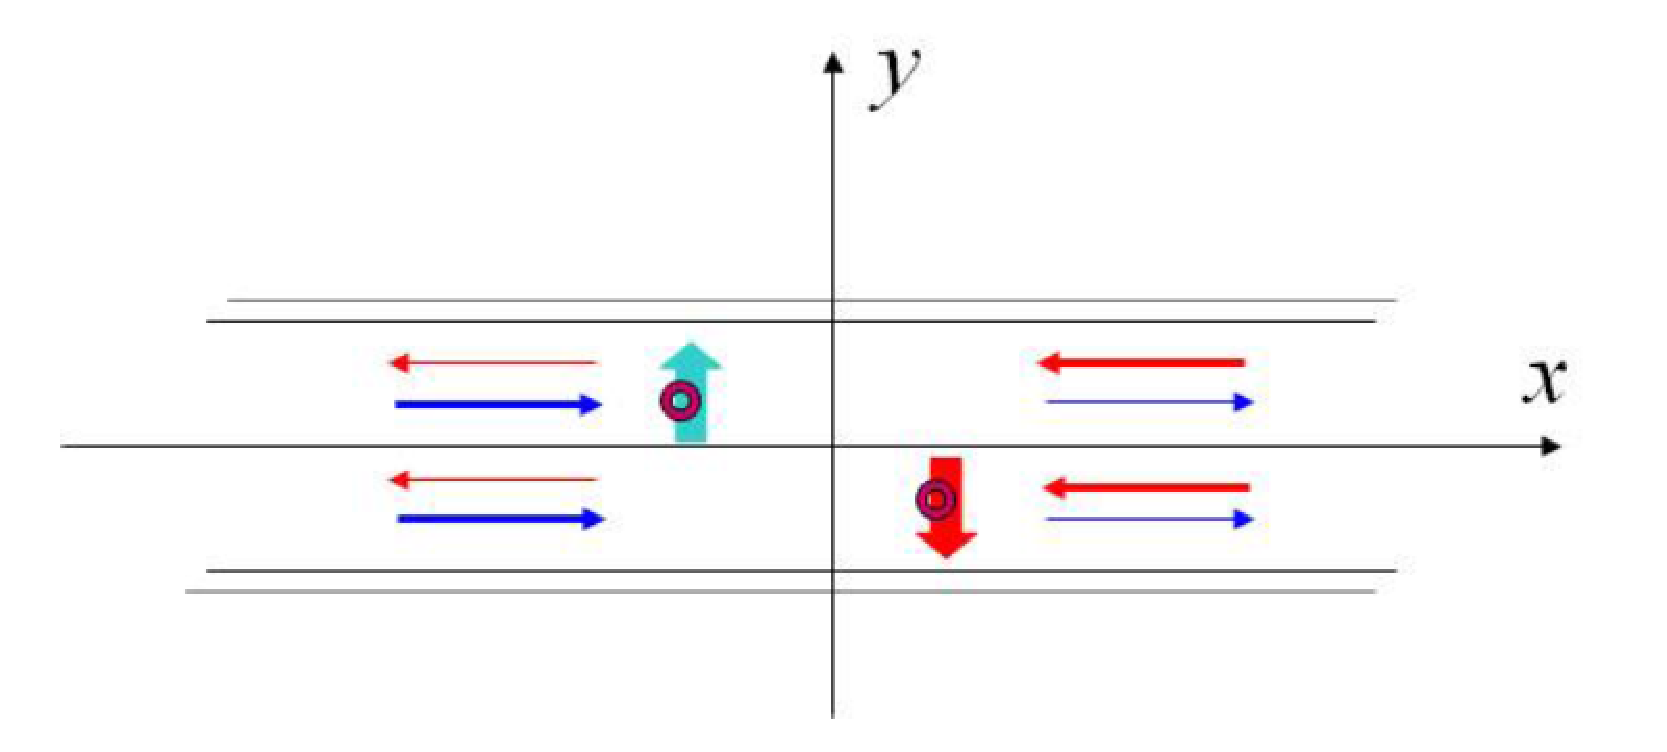
\includegraphics[width=10cm]{40.eps}
    \end{figure}
    \subsection{矩形海湾中的潮波}
    \subsubsection{宽度较窄矩形海湾中的潮波}
    \paragraph{假定和方程}~{}\\
    1. 海湾较窄\\
    2. 等深,深度为$h$\\
    3. 不考虑摩擦\\
    4. 密度为常数.
    \begin{figure}[H]
        \centering 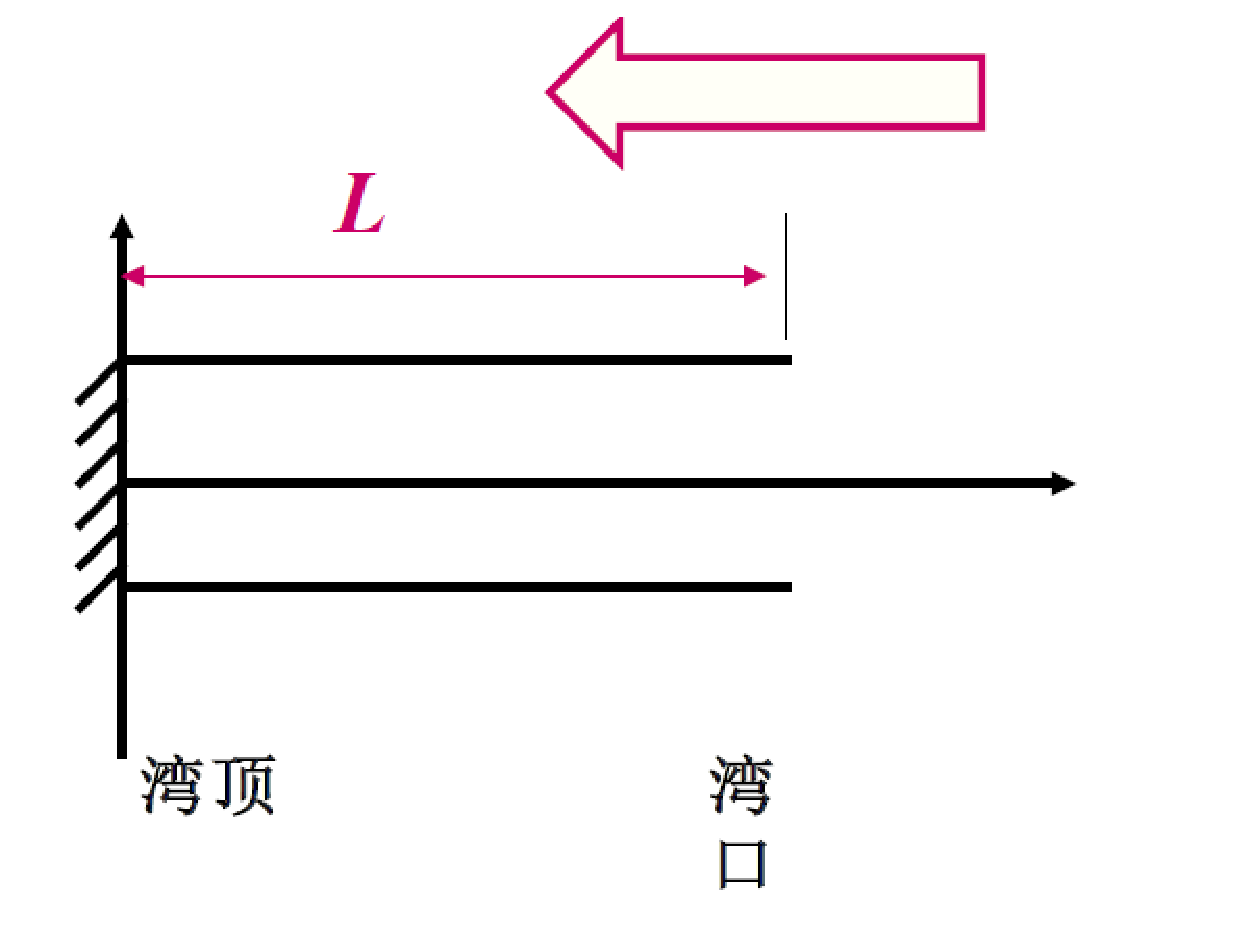
\includegraphics[width=10cm]{41.eps}
        \caption*{}
    \end{figure}
    \begin{numcases}{}
        \frac{\partial u}{\partial t}+g \frac{\partial \zeta}{\partial x}=0 \label{511}\\
            \frac{\partial \zeta}{\partial t}+h \frac{\partial u}{\partial x}=0\label{512}
    \end{numcases}
    边界条件:$\displaystyle \left.u\right|_{x=0}=0$
    \paragraph{求解}~{}\\
    研究一个分潮波:
    \begin{numcases}{}
        \zeta=Z(x)e^{i\omega t} \label{513}\\
        u=U(x)e^{i\omega t}\label{514}
    \end{numcases}
    \[
        {\partial (\ref{512}) \over \partial t}-h{\partial (\ref{511})\over\partial x}\Rightarrow {\partial^2\zeta\over\partial t^2}-gh{\partial^2\zeta\over\partial x^2}=0
    \]
    带入(\ref{513}):
    \[
        \frac{\partial^{2} Z}{\partial x^{2}}+\frac{\omega^{2}}{g h} Z=0
    \]
    令$\displaystyle k={\omega^2\over gh}$:
    \[
        Z=A_{1} e^{i k x}+A_{2} e^{-i k x}
    \]
    由(\ref{511}):
    \[
        U=-{g\over i\omega}{dZ\over dx}
    \]
    结合$Z=A_{1} e^{i k x}+A_{2} e^{-i k x}$:
    \[
        U=-\frac{g}{i \omega}\left(i k A_{1} e^{i k x}-i k A_{2} e^{-i k x}\right)=-\frac{g k}{\omega}\left(A_{1} e^{i k x}-A_{2} e^{-i k x}\right)
    \]
    边界条件$\displaystyle \Rightarrow A_1=A_2={R\over 2}$\\
    \[
        \left\{
            \begin{aligned}
                &\zeta=R\cos kxe^{i\omega t}\\
                &u=-i{gk\over \omega}R\sin kxe^{i\omega t}
            \end{aligned}
        \right.
    \]
    取实部:
    \[
        \left\{
            \begin{aligned}
                &\zeta=R\cos kx\cos \omega t\\
                &u={g\over c}R\sin kx\sin \omega t
            \end{aligned}
        \right.
    \]
    \paragraph{讨论}~{}\\
    1. 波动具有驻波性质\\
    2. 共振现象的机制.\\
    湾口:\[displaystyle \zeta_{B}=R \cos k L \cos \omega t=R_{B} \cos \omega t, \quad R_{B}=R \cos k L\]
    \[displaystyle \zeta=R_{B} \frac{\cos k x}{\cos k L} \cos \omega t=R_{B}\left(\cos \frac{2 \pi}{\lambda} x / \cos \frac{2 \pi}{\lambda} L\right) \cos \omega t\]
    \[
        \cos \frac{2 \pi}{\lambda} L \rightarrow 0 \Rightarrow \frac{2 \pi}{\lambda} L \rightarrow \frac{\pi}{2} \Rightarrow L \rightarrow \frac{\lambda}{4}
    \]
    当海湾的长度为潮波波长的1/4 时发生共振.
    \subsubsection{宽度较大的矩形海湾中的潮波}
    1. 需要考虑科氏力\\
    2. 通常为旋转潮波\\
    3. 潮波不仅仅是入射和反射Kelvin波的叠加,还要满足在湾顶的边界条件.\\
    Taylor半无限长矩形海湾潮波解由三部分组成:
    \[
        \left\{
            \begin{aligned}
                &\mbox{沿湾顶:湾口方向传播的Kelvin波叠加}\\
                &\mbox{一系列Poincare波之和}\\
                &\mbox{自湾顶向湾口以指数形式衰减的波动}
            \end{aligned}
        \right.
    \]
    \paragraph{矩形海湾中影响无潮点位置的因素}~{}\\
    1. 地摩擦效应:无潮点不再在海湾的中轴线上,面向湾顶向左偏\\
    2. 海湾横向水深梯度:无潮点偏向浅水一边.
    \subsection{变截面海湾中的潮波}
    \paragraph{结论}~{}\\
    1. 潮位由湾口向内逐渐变大\\
    2. 潮位振幅由湾口向湾顶增大,水深变浅比水深不变情况增大快.
    \subsection{总结}
    \begin{figure}[H]
        \centering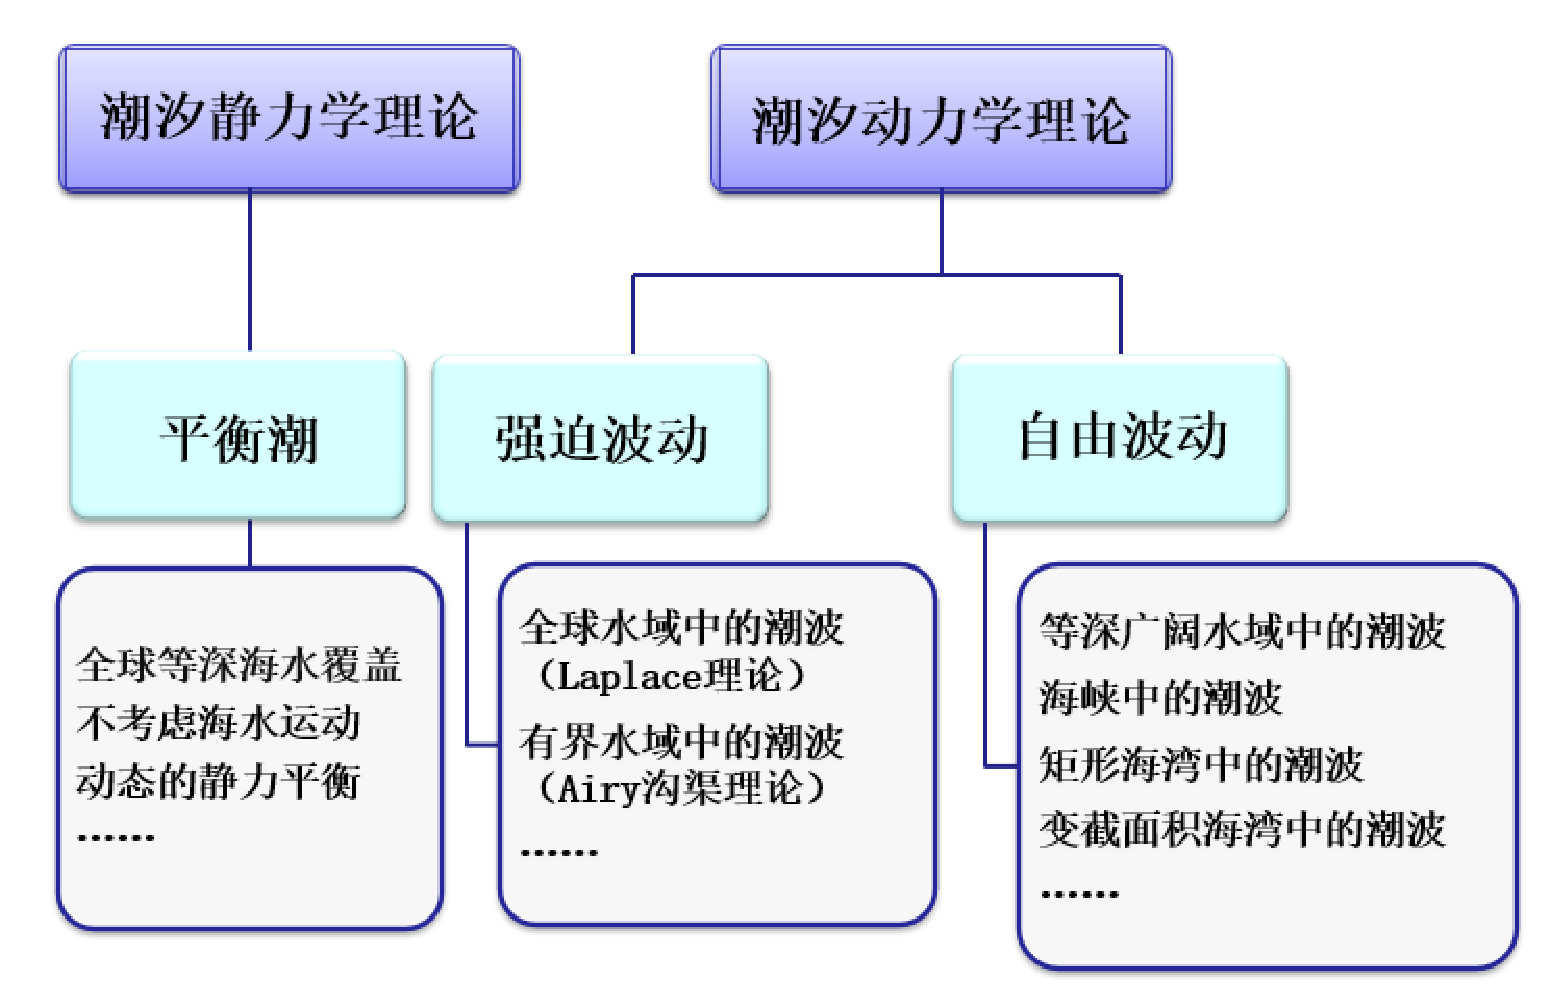
\includegraphics[width=10cm]{42.eps}
    \end{figure}
    \bibliographystyle{apalike}
	\bibliography{ref}
\end{document}